\svnkwsave{$RepoFile: siminos/spatiotemp/chapter/blogMNG16.tex $}
\svnidlong {$HeadURL: svn://zero.physics.gatech.edu/siminos/spatiotemp/chapter/blogMNG16.tex $}
{$LastChangedDate: 2020-07-02 12:19:27 -0400 (Thu, 02 Jul 2020) $}
{$LastChangedRevision: 6805 $} {$LastChangedBy: predrag $}
\svnid{$Id: blogMNG16.tex 6805 2019-03-17 20:54:15Z predrag $}

\chapter{Matt's 2016 blog}
\label{chap:blogMNG16}
% Predrag                                           26 May 2016

\bigskip

\hfill {\large Matthew N. Gudorf <matthew.gudorf@gatech.edu>}

   % *********************************************************************
\hfill   {\color{red} The latest entry at the bottom for this blog}

\section{Summer 2016 project description}
\label{s:summer16}

\begin{description}

    \PCpost{2016-05-22}{
\begin{description}
  \item[[x]] 2016-05-22 went through plane Couette
  \HREF{http://ChaosBook.org/tutorials} {tutorial}
  \item[[x]] numerically reproduce \KS\ evolution forward in time for
several finite $L$ periodic domains (use Xiong Ding codes)
  \item[[ ]] read ChaosBook.org chapter
\HREF{http://ChaosBook.org/paper.shtml\#PDEs}{Turbulence?}, very
critically! It aims to explain the relation between $L$ and the hyperviscosity
$\nu$, and it should be the fastest introduction to \KSe, for our
purposes, so blog %in \refsect{c-PDEs}
about what is unclear and what is missing.
% mark this box once you have entered a summary in \refsect{c-PDEs}
  \item[[ ]] summarize \KS\ in \refsect{sect:KStimeInt}
  \HREF{http://chaosbook.org/course1/Course2w16.html} {Course 2, week 16}
  might also be helpful.
  \item[[ ]] derive Michelson\rf{Mks86} ODEs and reproduce numerically
  some \eqva\ and \reqva\ for the $T=0$, spatially infinite domain
  \item[[ ]] Reading part of the project:
The best papers on $T=0$ seem to be
\begin{description}
  \item[[ ]] Michelson\rf{Mks86}
  \item[[ ]] Lan and Cvitanovi{\'c}\rf{lanCvit07}, summarize it here in
\refsect{sect:KSeqva}
  \item[[ ]] Lan\rf{LanThesis} thesis, summarize it here in
\refsect{sect:KSeqva}
  \item[[ ]] understand Dong and Lan\rf{DoLa14} {\em Organization of
  spatially periodic solutions of the steady {Kuramoto–Sivashinsky}
  equation} in detail, summarize it here in \refsect{sect:DoLa14}.
\end{description}
check off the boxes once you have read the above sources
and entered material learned from them either here, or in separate
sections (one for each source, as, for example, \refsect{sect:DoLa14})
  \item[[ ]] summarize $T=0$ in \refsect{sect:KSeqva}
  \item[[ ]] write a code that solves
 \KS\ evolution forward in space for finite $T$ periodic, spatially infinite domain
 (see \refsect{sect:KSspaceInt}; ask Burak for help)
  \item[[ ]] discuss the patterns that you see
  \item[[ ]] describe at length the $T\neq0$ results in \refsect{sect:KSspaceInt}
\end{description}
Matt, check off the boxes, with the date, as you complete them.
That, written up in your blog (this \emph{blogMNG16.tex} file), is good
enough for the completion of the Summer 2016 term project.
    }

    \PCpost{2016-05-22}{
If, in addition, you
\begin{description}
  \item[[ ]] reproduce some periodic
orbits and \PoincSec s for
$L=22$ periodic domain (use Xiong Ding codes)
  \item[[ ]] write up a literature survey, \refsect{sect:KSeqvaLit}
  \item[[ ]] compute any (by definition, new) {\po}s and/or {\rpo}s
for a fixed finite $T$ time-periodic spatial strip
  \item[[ ]] reduce the \On{2} symmetry of the \eqv\ equations
  (my impression is that no one in the literature has done that)
  \item[[ ]] there should be
also solutions that belong to invariant subspaces, much group-theoretical
analysis not done yet (that would mean that there are all kinds of
important \reqva\ that the literature has missed)
\end{description}
That is most likely worth a publication.
    }

\end{description}

\section{Matt's blog}
\label{sect:blogRS}

\begin{description}

    \MNGpost{2016-05-26}{
Here is an example of \MNGedit{text edit by me},
and here one of a footnote by me\MNG{2016-05-26}{test footnote}.
   }

    \MNGpost{2016-05-22}{
my SVN repo is {\em svn://zero.physics.gatech.edu/siminos}
\\
userID is
\texttt{mgudorf3}, the password is rather aspirational
    }

    \MNGpost{2016-05-22}{
Discussion with Predrag, \KS\ \eqva\ and \reqva\ project Summer 2016:
\begin{itemize}
\item blog the project progress here
\item blog whatever I'm reading and learning about
    dynamical systems here
\end{itemize}
    }

    \MNGpost{2016-05-23}{
 I've been working on reading the ChaosBook, so far chapts.~1 and 2.

 Considering doing the online Course 1.
    }

%    \PCpost{2016-05-26}{
%If you are taking notes on, or have a question about the ChaosBook or
%course material, enter it into \refchap{c-PDEs}.
%    }

\MNGpost{2016-05-22}{

\begin{itemize}
\item Installed Anaconda, Latex, Visual Studio to multiple machines.
\item Studied Movies of Plane Couette Tutorial
\end{itemize}

}

\MNGpost{2016-05-23}{

\begin{itemize}
\item Read Chapters 1,2 of Chaosbook
\item Read Nagata\rf{N90}
{\em Three-dimensional finite-amplitude solutions in \pCf:
bifurcation from infinity}. Describes the calculation of
the Nagata lower/upper branches pair of
equilibrium solutions to \pCf.
    \PC{2016-06-29}{A very technical paper, not (yet) relevant to your project.
        Do not worry if you do not understand parts of it}
\end{itemize}
}

\MNGpost{2016-05-24}{
\begin{itemize}
\item Video lectures for Chaosbook chap 1-2
\item Read Chapter 3
\item Gathered papers and resources for Computational Fluid Dynamics and
Kuramoto-Sivashinsky system
\end{itemize}
	}

\MNGpost{2016-05-25}{
\begin{itemize}
\item Video Lectures for Chaosbook Chapter 3
\item Began Working through Chaos Book HW1.
\end{itemize}
	}

\MNGpost{2016-05-26}{
\begin{itemize}
\item Finished Chaosbook: Homework 1 (server error couldn't submit)
\item Read Chapters 4, 5 Chaosbook
\item Read Dong and Lan\rf{DoLa14}, summarize it here in \refsect{sect:DoLa14}
\item Watched video lectures for Python learning via 1
\item Began reading Newman\rf{Newman12} {\em Computational Physics}
        (a python book)
        \PC{2016-06-29}{ask Xiong for what he likes as an introduction to python}
\end{itemize}
	}

%\MNGpost{2016-05-26}{
%%\textbf{Current Comments}
%%\begin{description}
%%\item[BlahBlah]
%\color{blue}
%Spent an (embarrassing) amount of time trying to access the repository,
%find my blog post file, and still can't get the .tex file to compile
%properly with all of the references; I'll ask adrien/rana/xiong what I'm
%doing wrong.
%%\end{description}
%	}

\PCpost{2016-05-26 Skype screen-sharing session}{
Showed how to use \emph{SVNtortioise}
(svn up, commit, log, diff), \emph{WinEdt} (master file, locate errors) and
\emph{JabRef}.
        }

\MNGpost{2016-05-26}{
%\textbf{Current Comments}
%\begin{description}
%\item[BlahBlah]
Still figuring out if I'm referring to articles properly.
	}

\XDpost{2016-05-27}{
For 1d \KS\ system,  you can start with
Kassam and Trefethen\rf{ks05com}
{\em Fourth-Order Time-Stepping for Stiff PDEs}. This
has a sample code to integrate \KS. You probably also need
to understand the pseudo-spectral method - a good introduction is
(you can look at my copy):
Trefethen\rf{trefethenSpectral} {\em Spectral Methods in MATLAB}.

Cvitanovi{\'c}, Davidchack and Siminos\rf{SCD07}
{\em On the {\statesp} geometry of the \KS\ flow in a periodic domain}
discusses \KS\ dynamics. You may have a look at
it and try to find the 2 \reqva\ by yourself.
    }

\NBBpost{2016-05-31}{
I agree with Xiong in that Matt should learn the essentials of the
pseudo-spectral methods as he will need to write his own integrator at
some point.

Kassam--Trefethen time-stepping scheme is elegant, also the
paper\rf{ks05com} is a good read, but it is not crucial since a generic
ode integrator does the job once the velocity function is correctly
defined.

For a fast start, Matt can run my (fortran + python and matlab), Xiong's
(cpp + matlab), and Ruslan's (matlab) codes in the siminos
repository, and pick one that suits his taste.

My matlab codes

\emph{siminos/ksConnected/ksETDRK4.m} (integrator, 73 lines)

and

\emph{siminos/ksConnected/vel.m} (velocity function, 26 lines)

might be easier to read because I calculate linear and nonlinear terms in
separate lines and calculation of nonlinear term is really all Matt needs
to understand.

As always, I'm available for skype/hangout whenever Matt might have a question.
    }

\PCpost{2016-05-31}{
Please try to keep Matt's workload within realistic bounds. Matt will have to
first write forward ODEs integration code for the time-periodic, $\infty$-space
\KS. Finding \eqva, \reqva, and {\po}s is another level, with a Newton code.
Let's postpone that (see the project outline in the beginning of this chapter,
edit as you see fit).
}

\MNGpost{2016-05-30}{.
\begin{description}
\item[Review] Took notes on \wwwcb{} Chapters 2-5 and Dong and Lan\rf{DoLa14}
         Watched video lectures for chapters 4-6. Edit: For week two of \wwwcb{}
\item[Learning] Read chapter 6, began reading chapter 14
    of \wwwcb{}, began video lectures for chapter 14.
    I'm trying to get to chapter 30 but I'm not sure if this is skipping too much
    but the book recommends only 2-5, 14, 15 to get to Chapter 30.
\item[Reading] Read and took notes (per Xiong's recommendation) on
Kassam and Trefethen\rf{ks05com}; planning on doing the same with
Cvitanovi{\'c}, Davidchack and Siminos\rf{SCD07} tomorrow.
\end{description}
    }

\MNGpost{2016-05-31}{.
\begin{description}
\item[Tangent] Went off on a tangent on materials way beyond the scope
    of my project (and most likely unrelated) before I brought myself
    back to Earth. Ranged from $C^*$-Algebras to KK-Theory to B{\'e}zier
    Curves. (I.E. Brownian Motion through Wikipedia)
\item[Reading] Began thorough reading of Cvitanovi{\'c}, Davidchack and Siminos\rf{SCD07}
\item[Review] Went over Kassam and Trefethen\rf{ks05com} notes
\end{description}
    }

\PCpost{2016-06-01}{
$C^*$-Algebras? Strongly unrecommended.
    }

\MNGpost{2016-06-02}{
\begin{description}
\item[Matlab]
    Downloaded and installed Matlab, spent time learning syntax and tried
    for some time to implement Matlab codes for \KS\ that Burak mentioned
    in {\bf Burak 2016-05-31},
    with an addition of a surface plot similar to Figure~6 of
    Kassam and Trefethen\rf{ks05com}.
    Produced a nonsensical plot; I believe it's because I don't know what
    to use for $x_0$.
\item[Learning]
    Reviewed some materials and completed \wwwcb{/course1} homework 2.
\item[Reading] Took some more notes on Cvitanovi{\'c}, Davidchack and Siminos\rf{SCD07}
\end{description}
    }

\MNGpost{2016-06-03}{
\begin{description}
\item[Matlab]
    Reproduced Figure~6 of Kassam and Trefethen\rf{ks05com}.
    Took a long time to debug a simple mistake but it was a good learning
    experience.
\item[Reading]
    Finished thorough notes on Cvitanovi{\'c}, Davidchack and Siminos\rf{SCD07}
\item[Comments]
    Am I writing these posts too often and/or should I reserve this space for more important messages? I don't want to make it a personal diary but I find it helpful for organizing what I've done so far.
\end{description}
    }

\PCpost{2016-06-04}{
That's great - more detail, rather than less, especially if you run into
something that you feel you do not understand well enough - there Burak, Xiong
and I can be of help.

Looks like you are moving right along - if your code produces something
that is qualitatively like Fig.~2.1 of Cvitanovi{\'c}, Davidchack and Siminos\rf{SCD07},
then you are ready to start coding equations of \refsect{sect:KSspaceInt}.
However, there is still much theory to read before you feel confident
about the results, see the project outline above, \refchap{chap:blogMNG16}.
    }

\MNGpost{2016-06-06}{
\begin{description}
\item[Learning]
Watched \wwwcb{/course1} video lectures for weeks 3, 4.
Read and took notes on \wwwcb{} chapters 7, 10, 11.

Went over notes on Cvitanovi{\'c}, Davidchack and Siminos\rf{SCD07} and
met with Predrag to talk about the bases with which visualizations are
produced. What I learned was it's better to get into the action by going
to points of interest (e.g. equilibria) and then look at their unstable
manifolds directly by projecting onto the respective eigenvectors. For
$2-D$ unstable manifolds this includes also using a third eigenvector
corresponding to the least contracting  eigenvalue/Floquet exponent, or
eigenvector with sufficient symmetry properties and contracting
eigenvalue.

\item[KS]
Played with the ETDRK4 code for \KS\ a bit more; varying parameters, size
of spatial domain, number of modes/spatial resolution, timestep.
Was able to reproduce for different spatially periodic domains.

I want to get a better idea of what I'm looking at. I believe I grasped a
better idea of what transient behavior looks like, because after a
certain time, there were no more distinguishable patterns no matter how
many modes I included, but the patterns after this critical time change
depending on the number of modes.
\end{description}

    }

\NBBpost{2016-06-06}{
I found this
\HREF{https://en.wikibooks.org/wiki/Parallel_Spectral_Numerical_Methods}{
wikibook}
a very practical introduction to the spectral methods for the solution
of PDEs. It starts with fundamentals and simple examples and goes all
the way to the parallel integration of Navier-Stokes equations in a 3D
box. Lectures also have accompanying Matlab/Python codes with them, and
the advanced parts have Fortran/MPI examples.
}

\PCpost{2016-06-07}{:

\begin{enumerate}
                      \item
The goal right now is to develop some intuition about spatiotemporal
turbulence, but not (as yet) write Newton codes for finding \eqva,
\reqva, and {\po}s.
                      \item
The goal of the project is to start simulating \KS\ on a finite
time-periodic, infinite configuration space  domain. (you would be the
first to do it, Burak and I believe). That would be a successful summer
project.
                      \item
The ultimate goal of the large research project is to take both time and
configuration space coordinates to infinity, and incorporate into this
PDE (for the first time for any PDE) Gutkin and Osipov\rf{GutOsi15} $2D$
discrete time, discrete space symbolic dynamics ideas.
                      \item
\emph{The dream} is to then port this to the infinite-length exact
turbulent Navier-Stokes pipe flow.
                    \end{enumerate}
        }

\MNGpost{2016-06-09}{
\begin{description}
\item[Review] Reviewed Chapters 7, 10, 11 of \wwwcb{}
\item[Meeting] Met and discussed projects with Rana and Adrien. Decided to meet up and discuss Ch. 14 of \wwwcb{} together on Monday.
\item[Reading] Read and took notes on \refref{Mks86}.
\item[Exercises] Completed Assignments 3 and 4 for \wwwcb{/course1}
\item[Additional]
Stumbled across some ways one could possibly improve Newton-Raphson
method such that it isn't as reliant on initial value.
A quote from: Abbasbandy \etal\rf{asNHAM07}:

``When the initial value $x_0$ is not good, comparing with the results
given by other methods, much fewer iterations are needed by HAM; even if
a bad initial approximation is chosen, which leads to divergent results
by other method, we can still find the root efficiently"

Similar applications are discussed by Wu and Chueng\rf{wc2ph10}
\end{description}

        }

\MNGpost{2016-06-10}{
Spent a lot of time messing around with matlab code on progressively
larger spatial domains to see if anything similar to Michelson\rf{Mks86}
popped up. For instance, when $L = 256 \pi$ what appears to be a
discontinuity in $u(x,t)$ develops at $x \approx 200$ and then at $x
\approx 200$ and $x \approx 600$, a distance $L/2$ away, turbulent
patterns emerge. I was trying to see if this had anything to do with the
discussion about bifurcations in Michelson\rf{Mks86} but I don't think I
know enough about bifurcations.
    }

\PCpost{2016-06-13}{
Instead of reading Michelson, it is probably easier to read the later
references I gave above (Lan, our papers, ChaosBook). There is no chance
now that you can see anything Michelson-related by integrating PDEs in
time - it applies only to $t=0$. However, it should be important for
study of the time-periodic PDE.

There can be no discontinuity in \KS\ evolution - hyperviscosity term in
the equation prohibits that. Presumably you are using too few Fourier
modes. Roughly speaking, if you double the domain lengh $L$, you should
double the number of Fourier modes in order
to attain the same accuracy...
    }

\MNGpost{2016-06-13}{
I don't know what I'm seeing then, as I made sure to be overzealous with
the number of modes. For $L = 256 \pi$ I used 20000 modes; it wasn't
really a discontinuity but just a region of sharp change in $u$. I
probably overlooked something else.

\begin{description}
\item[Learning] Read and took notes on chapters 12, 13, 14 \wwwcb{}
                Watched video lectures for weeks 5, 6 \wwwcb{}
\end{description}
    }

    \PCpost{2016-06-17}{
When in doubt whether a calculation returns a sensible answer, include
your plot / figure here, in the blog. Then Xiong, Burak and I can have a
look at it...
    }

\MNGpost{2016-06-13}{

Read \wwwcb{} Chapter 15
\\
Had a spatiotemp meeting
    }

\MNGpost{2016-06-13}{
Began my attempt to code space integration of \KS\ but quickly got
confused; The section \refsect{sect:KSspaceInt} presumes that we know
$u(x,t)$ and its derivatives for $t \in [0,T)$ ; Does this imply
that we know the initial conditions/analytic form of these
functions, and then evolve them at time at fixed $x$ to initiate the
grid of time values, and then commence the space integration?
    }

    \PCpost{2016-06-17}{
By construction, any temporal Fourier modes initial condition is
time-periodic with the fixed time period $T$. We have no very good idea
what the attractor looks like, so you can start with a first few Fourier
modes of order 1, rest 0. Or perhaps you can pick $T$ to be the shortest
(relative) \po\ \period{p} for $L=22$, take the time sequence at some
fixed $x$ as the initial condition (Xiong will tell you where it is in
this repository). We do not know what's a good starting guess. My hope is
that for $\period{} < \period{p}$, the time domain is too small to
accommodate spatiotemporal turbulence, and the attractor converges to a
Michelson-type $\period{}=0$ spatially chaotic strange set (no interesting
time dynamics).
    }


\MNGpost{2016-06-13}{
    \begin{description}
    \item[KSspaceint]
    Spent most of the day trying to code spatial integration. I have the part that takes in data for the velocity function $u(x,t)$ and its derivatives down. Trying to apply fourth order Runge-Kutta on the rest; It likes to blow up to infinity, when I put in even dumber initial conditions it still likes to blow up. I believe this is due to one of three things:
    \begin{enumerate}
    \item Runge-Kutta is insufficient in it's accuracy.
    \item Not handling the non-linear term correctly.
    \item Not handling time derivative term correctly.
    \end{enumerate}
    Will attempt to reach Burak soon.

    \item[Spatiotemp]
    Meeting: I came in late due to real life but the gist of what I gathered was the procedure on how to get inequalities to generate lines in order to describe the certain fixed symbols in a sequence. When a symbol is fixed, the area bounded by these lines describes the frequencies of that symbol. Longer chains of symbols generate more lines, and more conditions/rules on which pieces of area are of interest. The general formulae involve Chebyshev polynomials. Adrien and Rana are going to look for
    [$2 \times 2$] squares next I believe.

    \item[Sidenote]
    I'm getting some sort of error with siminos.bib that won't allow me
    to compile the blog. I would try to fix it myself but I'm unsure what
    the error message means.
    \end{description}
    }
    \PCpost{2016-06-21}{
``some sort of error'' does not cut it as an explanation to the IT squad.
If it is a comma that Xiong forgot, I fixed it now. You can fix such
errors yourself, the error message tells you what line of the *.bib file
to fix. But, if you have not edited \emph{siminos.bib} and are getting
such errors, try going to \emph{siminos/bibtex/},  remove all
\emph{siminos.bib*} files, svn up. Should fix it.
    }

\NBBpost{2016-06-17}{
    The numerical instability was something that I was expecting. While
    the points you mentioned can definitely cause it (especially make
    sure that you treat all terms correctly), there is an obvious
    difficulty with \refeq{e-ksX}, that is the absence of the diffusion
    term. Let us have a look at the original \KSe\ in the Fourier space
    \beq
        \dot{\Fu}_k = (q_k^2 - q_k^4) \Fu_k
                    - \frac{i q_k}{2} \mathcal{F}\{u^2\}_k \, \quad
        \mbox{where, } q_k = 2 \pi k / L \, , \Fu_k = \mathcal{F}\{u\}_k
        \, . \label{e-Fksex}
    \eeq
    Now pay attention to the coefficient of the linear term:
    \beq
        q_k^2 - q_k^4 = \frac{(2 \pi)^2 k^2}{L^2}
                      - \frac{(2 \pi)^4 k^4}{L^4} \label{e-clinear}
    \eeq
    If we set \refeq{e-clinear} to $0$, we find $k = L / 2 \pi$;
    for $k$ smaller than this value, \refeq{e-clinear} is positive
    and negative if $k > L / 2 \pi$. For large enough $k$, this term
    falls down as $k^4$, dominating everything and strongly damping the
    high Fourier modes. This is the main justification of using a finite
    Fourier mode truncation for the numerical study of \KSe.
    In many PDEs with diffusion (second order space derivatives),
    this damping goes like $k^2$, however, in \KSe\ \refeq{e-ks} ,
    the second-order space derivative has negative sign, thus it
    supplies energy to the low wave numbers (negative diffusion), while
    the energy is dissipated like $k^4$ (hyper diffusion) at higher
    ones. Another consequence of this fact is time-irreversibility:
    In principle, we have a deterministic PDE at hand, present (an
    initial condition) describes future perfectly well, so we may expect
    to recover the initial condition if we know the final one. However,
    this is may not be the simple task of backwards-integrating
    \refeq{e-Fksex} in time. The reason is once we reverse the arrow of
    time, the negative diffusion vs. hyper diffusion story becomes the
    opposite and we supply energy to the system at higher and higher
    Fourier modes which are all unstable, hence no finite-truncation
    can be justifiable.

    With this in mind, let us look back at \refeq{e-ksX} and
    \refeq{e-FksX}. You can see that there is no (hyper)diffusion term
    that damps Fourier modes corresponding to high frequencies. There is
    no obvious production term (energy supply) either, but still control
    of numerical accuracy in this case is not as obvious as it was for
    the spectral discretization in space. The similar situation appears
    for advection equations in fluid mechanics and one way to deal with
    that is adding an ``artificial diffusion'' term, such as
    $\epsilon u^{(3)}_{tt}$ to the RHS of the first equation in
    \refeq{e-ksX}, which would show up as
    $- \epsilon \omega_k^2 \Fu_k^{(3)}$ in Fourier space. Once you do that,
    of course, there is a new parameter to experiment with. You should
    make sure that $\epsilon$ is small enough so that it's effect for
    long time scales (low frequencies) are negligible and it effects
    only very-high frequency modes, that corresponds to the time scales
    you don't really care.

    Once you make sure all your terms are correct, please try adding an
    artificial diffusion term to the equation and see if it stabilizes
    the numerics. We can then check if it gives a numerically correct
    result by comparing it to time-integrated results.
    Also please \color{red} commit your code\color{black}.

    Another potential problem we might have is so-called ``aliasing'',
    that is generation of artificial sub-harmonics from the
    finite-truncation of the nonlinear term (you can learn about it
    from any pseudospectral methods for PDEs book, see for instance
    \refref{Canuto88}).
    This may or may not cause numerical instability issues but certainly
    has an effect on the accuracy. But hopefully is secondary at this
    level.

    This, by the way, was my main concern about insisting on having an
    initial condition from a time-integrated simulation, because in
    time-evolution, we know that high Fourier modes damp and the flow
    is driven towards an energy-balanced (on average) chaotic attractor.
    We don't have such a guarantee in space-integration, and that's why
    I was thinking we should start with a point on the attractor.
}

    \PCpost{2016-06-21}{
email to Lan Yueheng <lanyh@bupt.edu.cn>, Skype yueheng\_lan :

Matt, a graduate student here, is reading your \KS\ papers (with me and
Dong) and your thesis, parts on the Michelson strange attractor that
describes $T=0$ equilibria for infinite spatial domain. Burak and I have
not decided to whether to first look at it in the reflection
antisymmetric invariant subspace $\bbU^+$ (as we did - probably preferable, as
there are no relative equilibria, no relative periodic orbits and no
continuous symmetry to quotient), or study the full $\On{2}$-equivariant
problem.

I'm going away for a few weeks, a real vacation - do you mind helping
Matt by Skype (matthew.gudorf) or whatever is convenient? It's a lot of
material to master, and he has no background in nonlinear dynamics.
    }

\MNGpost{2016-06-21}{:

%    \begin{description}
     {\bf KSSpaceInt}
%    \color{red}
    After shedding much sweat and many tears I think I made a little bit
    of headway into the integration process. There are still many
    problems but I can at least generate a plot for very limited sizes of
    spatial integration i.e. $L = 2$ with step size $.01$.
    %I could be doing this completely wrong/thinking about it the wrong
    %way because I'm not that great at coding.
    I'm going to include my matlab files,
    % if I can figure it out in my tired state,
    that include many comments
    on what I'm attempting to do. the main Matlab file is
    \texttt{timeperiodic.m} so if you have the other two files around and plug
    in the initial conditions indicated at the top you'll be able to see
    what I see; I'm not sure how to include figures directly into the
    blog.
%    \end{description}
    }

\MNGpost{2016-06-23}{:
    \begin{description}
    %\color{red}
    \item[Meeting with Burak and Predrag]
    Talked about the progress so far, explained my Matlab code
    \texttt{timeperiodic.m} for the spatial integration of \KS\ a fixed
    finite $T$ time-periodic spatial strip.

    My strategy, in order to initialize the $x$ integration of
    \refeq{e-ksX}, was to time-integrate $L=22$ \KS\ for
    $t\in\{0,1000\}$, store this as a large matrix, decide by eyeballing
    that transients have died out by $t=t_{in}=400$, take
    $t\in\{t_{in},t_{in}+T\}$ column of values of $u(x_0,t)$, where
    $x_0=250$, arbitrarily picked,  and $T=??$, all in my own units. Fourier
    transform $u(x_0,t)$ to $\tilde{u}(x_0,k)$, assuming periodicity in
    $T$, construct from it $\tilde{u}_{x}(x_0,k)$, $\tilde{u}_{xx}(x_0,k)$
    and $\tilde{u}_{xxx}(x_0,k)$, then Fourier transform these back to
    discretized time-vector
    \beq
    ({u}(x_0,t),{u}_{x}(x_0,t),{u}_{xx}(x_0,t),{u}_{xxx}(x_0,t))
    \ee{U_mx}
    $t\in\{0,T\}$ time-periodic strip. These 4 spatiotemporal fields are
    then integrated forward in $x$ using \refeq{e-ksX} and my own
    Runge-Kutta routine (no FFTs).

    Burak was cool with all of this. Still, the time Fourier modes seem to explode.
      Some of the talking points:
        \begin{enumerate}
        \item Use real time and space units instead of the number of
            discretization steps.
        \item Improve the notation for the variables.
        \item  For a space integrator, use a built-in Matlab integrator
            such as ``ODE45" as opposed to my manually coded fourth-order
            Runge-Kutta.
        \item My ergodic segment $u(x_0,t)$ is discontinuous (a
            Heaviside function discontinuity) at $T \to0 $ point, and so
            are ${u}_{x}(x_0,t),{u}_{xx}(x_0,t)$ and ${u}_{xxx}(x_0,t)$.
            That means that Fourier spectrum will be essentially flat to
            arbitrarily high frequencies, and useless as an initial
            condition. Burak's diffusion regulator might mitigate some of
            that, but in any case, regularized initial condition will be
            off the strange attractor.
         \item Perhaps pick $t_{in}$ by requiring that it corresponds
            to a close recurrence in time direction, $u(x_0,t_{in})
            \approx u(x_0,t_{in}+T)$, as a possible initial condition on
            a time-strip? Probably continuity in $u(x_0,t)$ alone does
            not help, as $u_t(x_0,T)$ and higher derivatives in $t$ are
            still discontinuous, Fourier transform does not like that
            either.
         \item Use a cubic spline through a range of points spanning across the
            point of discontinuity $u(x_0,T)$. This, however, would
            necessarily lift us off of the attractor, which was the whole
            point of waiting that time-transients die, etc.
        \item  Taking into account all of the above problems of
            picking good initial $t=0$ time-vector \refeq{U_mx}, we gave
            up on initialization by a time-segment of an ergodic
            trajectory, and decided to use Xiong periodic orbit data for
            one of the shortest $\period{p}$ {\rpo}s or {\ppo}s on the
            $L=22$ spatial strip as an initial condition.
        \item Will have to time-reintegrate Xiong \po\ using $\Delta t =
            \period{p}/2^{M}$ time-step to set up time-discretization
            needed for a spatial direction pseudo-spectral FFT
            integrator.
        \item How do we know that the integrator in space is working?
            It presumably has to reproduce the initial $u(x_0,t)$ and its
            derivatives at $u(x_0+L,t)$ and its repeats  $u(x_0+mL,t)$.
            If this is correct, it should also give us some sense of the
            stability of the $u(x_0+x,t)$ orbit in the $x$-evolution.
        \item Boris says that in a secret document he has shown that for
        a spatiotemporaly periodic solution (a torus that tiles the
        spacetime)
\beq
\det (1-J) = \det (1-K)
\,,
\ee{BGsecret1}
            where the \jacobianM\ $K$ is computed for the
            linearization of the evolution in the $x$, spatial direction.
            That would be an additional check on the integrator.
        \item Will have to think what does it mean to start with an \rpo?
        The tiling is by parallelepiped rather than by rectangles. Can
        cheat by starting with a \po\ obtained by a repeat of an \ppo.
        That's considered good enough for government work.
        \end{enumerate}

    \item[Exercise]
        Derive \refeq{BGsecret1}. You get Lenin Medal for that.

    \item[Discussion with Xiong]
    Xiong showed me where the codes for his time integration are and how
    to retrieve the data for periodic orbits from a file. I'll need to
    install a linux virtual machine image to run the time integration
    code.

    \end{description}
    }

\MNGpost{2016-06-24}{:
    {\bf KSSpaceInt}
Worked all day to try and get \texttt{ksint.m} to run. With some help from my brother (who is also a code guru) I created a virtual image that runs 64 bit Ubuntu as well as a shared folder between my current Windows operating system and my Ubuntu virtual image.

I believe that I need Ubuntu to run \texttt{MEXksint.mexa64} which is called in previously mentioned MATLAB function, but there seems to be a problem with some missing libraries which I was unable to locate; due to how they are imported it looks like they are some custom made files and not MATLAB libraries. I e-mailed Xiong about this and hope to clarify this issue so that I will have some results come Monday.
    }

    \PCpost{2016-06-24}{
It would be easier (and faster in the long run) to do this on the
CNS linux cluster. Your userID is \emph{gudorf}, I emailed you the password separately.

You can use the linux box in the second bay to the left in
the grad students office W503 (if Kinsey is not there),
or linux terminal in the computer cubicle W508E (Xiong has the key),
or Boris Gutkin's linux box (he is never there before 4-5 pm :) in W501B.
Login as \emph{gudorf}. Then
\emph{ssh -X gudorf@hard.physics.gatech.edu}; that puts you into Xiong's
linux box which has all the packages you need already installed.

If you start generating lots of data, store it locally, somewhere in

\emph{/usr/local/home/gudorf/}

You can get there by \emph{cd localHard}. That is needed because your
home directory is backed up every night, and if there are
Mr. Rump-self-perception size files in it, it will break the backup for
everyone.

If not using a CNS linux box,
\HREF{http://www.cns.gatech.edu/CNS-only/VPN.html}{VPN} to get past the
firewall. Then \\
\emph{ssh -X gudorf@zero.physics.gatech.edu}
\\From there,\\
\emph{ssh -X gudorf@hard.physics.gatech.edu}
\\
This \emph{-X} enables you to open
the \emph{hard.physics.gatech.edu} Matlab etc. on your own laptop, provided ...
(simpler you talk to Xiong about it).

    }

\MNGpost{2016-06-24}{

\begin{description}
\item[KSspaceint]
Revamped my code over the weekend and debugged today with help of Xiong.
Solutions still blow up past $L=12$ and are not very descriptive past $L
\approx 8$. In \reffig{fig:MNGspaceIntL22}
I show $u(x,t)$ resulting from my curreent spatial
integration of $u^{(\ell)}(x_0,t)$ for the periodic domains
$T= 2\,T_{\PPO{10.2}} =20.5058$ and
$T=4\,T_{\PPO{10.2}} = 41.0116=2*T_a$
and $x_0=11$ (by random choice of
spatial grid coordinate $x_i = 16$, $1 \leq x_i \leq 32$).
%I hope to get a more useful result tomorrow but I had been coding/debugging
%for twelve hours and decided to leave it at that for the day.
Fourier modes are my
next objective, which will be easier.
% in fact and I'm surprised I didn't do it first.

\begin{figure}
  (a) 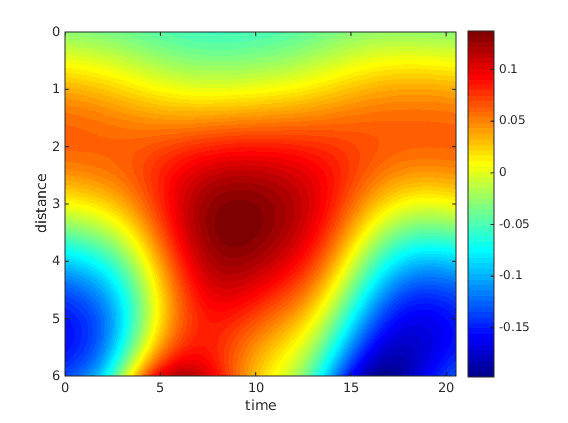
\includegraphics[width=0.45\textwidth]{MNG1periodL22}
  (b) 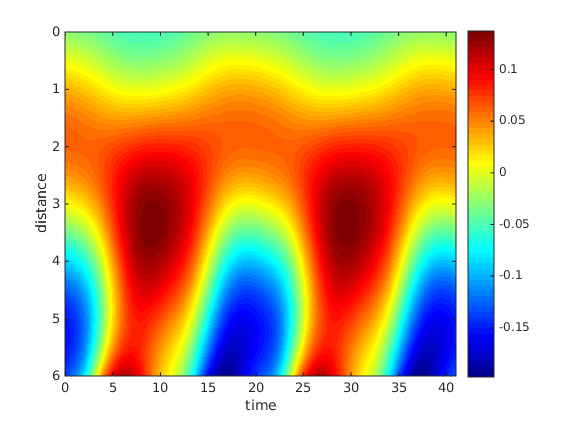
\includegraphics[width=0.45\textwidth]{MNG2periodL22}
\caption{
Spatiotemporal plots of $u(11,t)$; for the spatial integration of
\refeq{e-FksX} for time periodic-domains
(a) $T= 2\,T_{\PPO{10.2}} =20.5058$ and
(b) $T=4\,T_{\PPO{10.2}} = 41.0116$, from $x=0$ to $x=6$ (starting at the top).
The initial $u(11,t)$
are given by the $\PPO{10.2}$ time profile at $x=11$.
This is a reproduction
\PCedit{(PC what is ``reproduction?'')}
of Xiong's code \texttt{ksint.m} along with
application of fast Fourier transforms and their inverses.
\label{fig:MNGspaceIntL22}
}
\end{figure}

\item[Concerns]
\begin{enumerate}
 \item
 I don't know what the order of magnitude is considered large for the artificial diffusion constant $e$ so I went with $e=0.1$, will talk to Burak to get a better idea.
\item
Even with using \texttt{ode45.m} in MATLAB, the solutions still diverge at $L \approx 12$. Past $L \approx 6$ the plots of $u(11,t)$ became very undescriptive as the magnitude begins to diverge. Will try implementing \texttt{ode15s.m} which deals with stiff differential equations better than (\texttt{ode45.m} unless there is a better suggestion.
\end{enumerate}
\end{description}
    }

\MNGpost{2016-06-24}{

\begin{description}
\item[Meeting with Burak]
Burak and I discussed the current problems I am having and also questions I had regarding \KS\ spatial integration.  The main pieces of advice were as follows:
\begin{itemize}

\item Should verify that the truncation of Fourier modes is reasonable,
i.e. the amplitudes decrease towards zero. Recommended that I plot the
logarithm of the Fourier mode amplitudes to look at their initial values.

\item An implicit integration method might need to be deployed because
explicit methods can be unstable. Burak suggested to look at both the
``Implicit Midpoint Method" and ``Fixed Point Iteration Method".
\BB{2016-06-25}{
Implicit midpoint method is a symplectic integrator, which is appropriate
for Hamiltonian dynamics. When you implement it, you get an algebraic equation
for the next step in integration, one way of solving for the next step is
``Fixed point iteration''. There might be better methods.
}

\item Also
mentioned Symplectic Integrators because they are energy-preserving. Noted
that I should probably start with the artificial diffusion term should be
zero when I begin these implicit methods, although that will probably be
inaccurate when integrating over large spatial domains.

\end{itemize}

 \item[Initial Fourier mode amplitudes]
 The following is the initial Fourier mode amplitudes plotted against their
 frequencies on a logarithmic scale. The zero-frequency mode dominates and
 I'm not sure if that is problematic or not.

 \begin{figure}
    \centering
    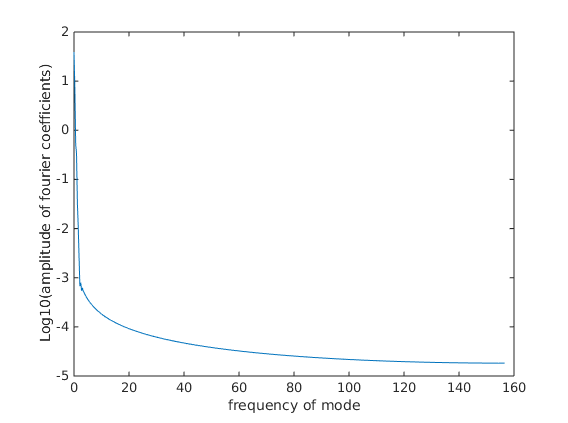
\includegraphics[width=0.65\textwidth]{MNGinitialfourier}
    \caption{
    Initial amplitudes of Fourier coefficients of temporal Fourier modes
    (512 positive frequency modes) for two periods of the shortest
    \ppo\ $\PPO{10.2}$, plotted on a logarithmic (base 10) scale. }
    \label{MNGinitialfourier}
 \end{figure}

  \item[KSspaceint]
  More attempts at trying to get my spatial integration code to work so that
  the temporal Fourier amplitudes do not diverge/blow up.

  Switching from \texttt{ode45} to \texttt{ode15s} had little to no effect. Attempting to correct for aliasing by zero-padding when calculating the nonlinear term via pseudo spectral method. That is, when calculating:

  \beq
  \sum_{m = -\infty}^{\infty} \Fu^{(0)}_{k - m} \Fu^{(1)}_m
        = \mathcal{F} \left\{ \mathcal{F}^{-1} \left\{\Fu^{(0)} \right\}
                              \mathcal{F}^{-1} \left\{\Fu^{(1)} \right\}
                      \right\} \, ,
  \eeq

  The "zero-padding" process can be described as the following: Firstly we add extra elements, which are equal to zero, to each array representing $u^{(0)}$ and $u^{(1)}$
  (the length of each array is determined by the temporal resolution, let's call it $N$). Typically, the number of zeros we add is equal to (or greater than) the original number of elements in each array. After "padding" with zeros, each array now contains $2N$ elements. The inverse FFT's are then applied is the equation above, as well as the convolution. The next step is to apply the FFT to the convolution, leaving us with an array that still has $2N$ number of elements. The final step is to prune $N$ elements away so that the final result has $N$ elements. This is done to
  eliminate artificial sub-harmonics produced by finite truncation of Fourier modes.

  Sadly, this did not seem to help the lack of damping and divergence was still present.
  \end{description}
  }

\NBBpost{2016-07-02}{
Zero-frequency mode is the average value of the initial signal. I don't see a
problem with it having a large value.
Please give us more detail about what is on \reffig{MNGinitialfourier}, does
the initial condition correspond to two periods of the shortest \ppo\ $\PPO{10.2}$? How many Fourier modes are there? Does it go below 5 orders of magnitude
drop-off if you include more modes?
}

\MNGpost{2016-07-04}{

    \begin{description}
    \item[KSspaceint]
    Spent the day trying to figure out the best way to compute the convoluted sum on the left hand side of following equation:
    \beq
    \label{e-KScp}
    \sum_{m = -\infty}^{\infty} \Fu^{(0)}_{k - m} \Fu^{(1)}_m
        = \mathcal{F} \left\{ \mathcal{F}^{-1} \left\{\Fu^{(0)} \right\}
                              \mathcal{F}^{-1} \left\{\Fu^{(1)} \right\}
                      \right\} \, ,
    \eeq
    and keep my code consistent. Wrote this in \texttt{convolutionsum.m}.
    Sort of worried about how trying to evaluate an infinite sum with a truncated number of modes.

    In order to keep the code consistent I also edited \texttt{timeperiodic.m} by reordering the Fourier mode from negative frequencies to positive frequencies. Hopefully this will solve once and for all the problem of whether my Fourier modes are normalized correctly. I keep finding conflicting notation, no doubt due to the difference in conventions between engineers and everyone else.

    \item[Misc.]
    Edited the caption for the \reffig{MNGinitialfourier}, will try adding more Fourier modes to see how the amplitudes behave.
    \end{description}
    }

\PCpost{2016-07-05}{
I am a bit worried about \reffig{MNGinitialfourier}, where the modes
flatten out to about $10^{-4.7}$. That presumably means that the initial
condition -should have been on the domain $T= 2\,T_{\PPO{10.2}}
=20.5058$- is not smoothly periodic, but it someplace has either a
$\delta$-function singularity, or - more likely, a Heaviside
$\theta$-function step? A good initial time-periodic $u(x_0,t)$ should
fall off at least exponentially, with Fourier modes leveling off only at
the machine precision. And I doubt one needs 512 modes (I assume that
means 256 complex Fourier modes?). I would have guessed that 64 would
have been plenty...

Consult with Xiong about the quality of your initial $u(x_0,t)$
``periodic'' profile? You have to be much more explicit about what you and
Xiong did to $\PPO{10.2}$ to obtain your initial $u(x_0,\cdot)$ for Burak
and me to ponder what went wrong. While you are at it, perhaps do not
pick arbitrary $x_0=11$ initial $u(x_0,\cdot)$. When you look at the time
evolution of $\PPO{10.2}$ on the $L=22$ domain, pick initial $x_0$ such
that $u(x_0,t)$ looks as smooth as possible (not sure that what I
recommend here really matters).
    }

\PCpost{2016-07-05}{
Your $T= 2\,T_{\PPO{10.2}} =20.5058$ in \reffig{fig:MNGspaceIntL22}\,(a)
initial should be strictly periodic, I agree. But there is no need to yet
again double the size of the periodic domain, as in
\reffig{fig:MNGspaceIntL22}\,(b). That is asking for more trouble than
needed right now.

The good news is that your evolution of the two domains is consistent.
    }

\PCpost{2016-07-05}{
Why from $x=0$ to $x=6$, when the initial $u(x_0,t)$ are given by the
$\PPO{10.2}$ time profile at $x_0=11$?

You sure that it is $u(x_0,t)$ ``starting at the top?''. Judging by the
color scale on the right, the initial $u(0,\cdot)$ is essentially flat,
and it is still rather small by $u(6,\cdot)$: I do not remember $u$ to be
so small in magnitude, but my memory can be wrong. You can crosscheck
with plots in Cvitanovi{\'c}, Davidchack and Siminos\rf{SCD07} whether
your $u$ magnitudes are what they typically see.
    }

\item[2016-07-05 Xiong]
Matthew had a question about FFT used in my code.
\begin{quotation}
  Hey Xiong,

  I know we discussed the matlab file ksint.m in detail, and it is working well, but I have a question that you might be able to help me with.

  The inverse fast Fourier transform implemented by MATLAB divides the result by N where N is the number of modes. I am applying this inverse transformation to values returned by ksint.m, and I'm unsure how the normalization should be treated in order to recover the correct values for u(x,t).

  I have a suspicion that I need to multiply the results by N in order to cancel out the division by N from IFFT, this is because otherwise the initial values seem too small, on the order of hundredths.

  If you have any idea I would be very thankful!

  -Matt
\end{quotation}

The truth is that the normalization convention of
discrete Fourier transform I am using is
different from the standard one. The reason is that I need to
keep my code consistent with the code and data provided in folder
\texttt{siminos/matlab/ruslan}, which is also the convention used
in \refref{SCD07}.
I almost forget this difference
after identifying it 3 years ago.
Please search \texttt{2013-08-01} in \texttt{siminos/lyapunov/blog.pdf}
to see the details.

PS Compile it first. \texttt{cd sinimos/lyapunov \&\& pdflatex blog.tex}.

\begin{figure}[h]
  \centering
  \begin{minipage}{.32\textwidth}
    \centering \small{\texttt{(a)}}
    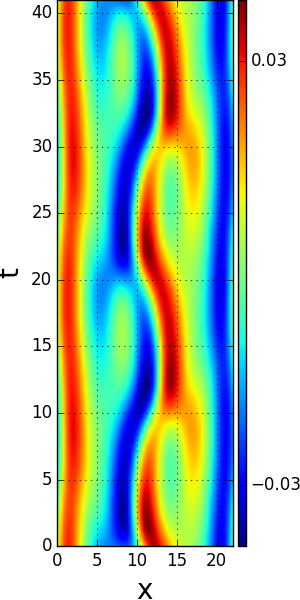
\includegraphics[width=\textwidth]{ppo1State64}
  \end{minipage}
  \begin{minipage}{.32\textwidth}
    \centering \small{\texttt{(b)}}
    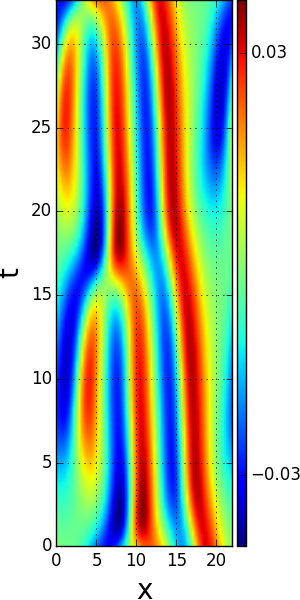
\includegraphics[width=\textwidth]{rpo1State64}
  \end{minipage}%
  %\begin{minipage}{.55\textwidth}
  %  \centering \small{\texttt{(c)}}
  %  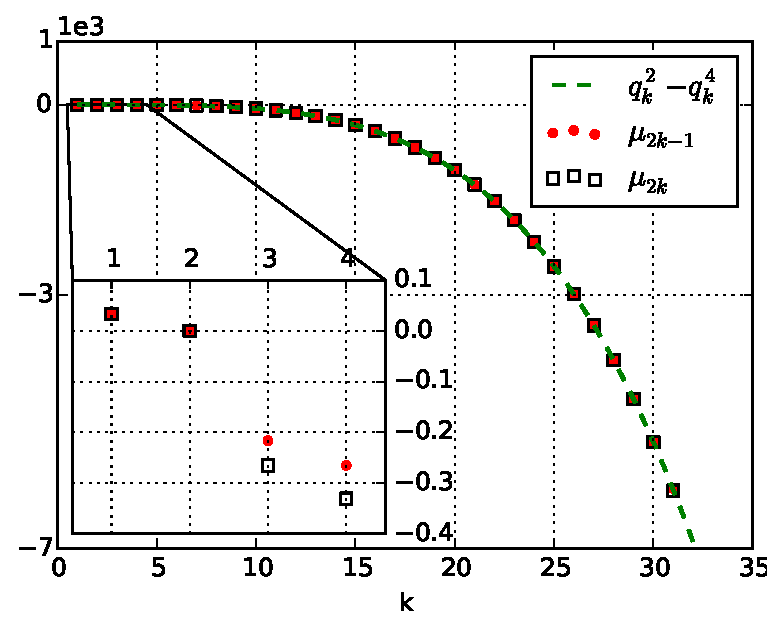
\includegraphics[width=\textwidth]{ppo1spectrum64}
  %\end{minipage}
  \caption{ %(Color online)
    (a) Pre\po\ $\cycle{pp}_{10.25}$ and
    (b) \rpo\ $\cycle{rp}_{16.31}$ for total evolution time
    $4\,\period{pp}$ and $2\,\period{rp}$, respectively. The \edit{spatial} shift
    for $\cycle{rp}_{16.31}$ after one prime period $\simeq-2.863$.
%    (c) The real parts of Floquet exponents paired for a given $k$ as
%    $(k,\eigRe[2k-1])$ and $(k,\eigRe[2k])$, for $\cycle{pp}_{10.25}$ with
%    truncation number $N=64$. The dashed line (green) is
%    $q_{k}^{2}-q_{k}^{4}$. The inset is a magnification of the region
%    containing the 8 leading \edit{exponents}.
    From Ding and Cvitanovi{\'c}\rf{DingCvit14}.
  }
  \label{fig:ppo1rpo1}
\end{figure}

\PCpost{2016-07-05}{
The first test is to see whether your \emph{time} integration reproduces
\reffig{fig:ppo1rpo1} over the $t\in [0,2\,T_{\PPO{10.2}}]$ time
interval, starting with Xiong's data set for $\PPO{10.2}$. If that is
working, a vertical line for some $x_0\in [0,22]$ is used for initial
$u(x_0,\cdot)$ for \emph{space} integration. If the integrator is
working, the updated version of \reffig{fig:MNGspaceIntL22}\,(a) should
coincide with \reffig{fig:ppo1rpo1}\,(a) over the $x\in [0,22]$ space
interval. That would be enough to declare victory for this summer
project.
    }

%%%%%%%%%%%%%%%%%%%%%%%%%%%%%%%%%%%%%%%%%%%%%%%%%%%%%%%%%%%%%%%%%%%
%\begin{figure}[t]
%\begin{center}
%%  (\textit{a})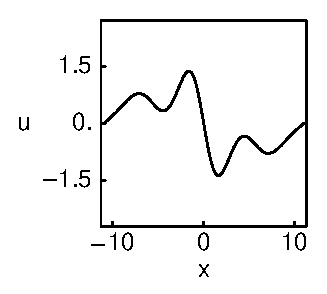
\includegraphics[width=0.35\textwidth, clip=true]{figs/1wKS22equil.eps}
%%~~~~(\textit{b})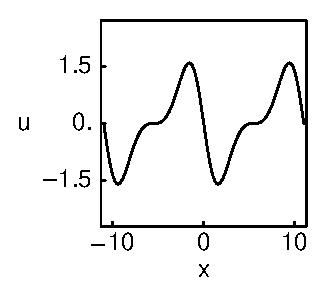
\includegraphics[width=0.35\textwidth, clip=true]{figs/2wKS22equil.eps}
%%\\
%%  (\textit{c})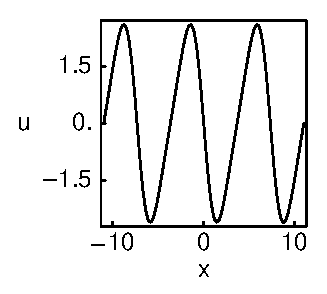
\includegraphics[width=0.35\textwidth, clip=true]{figs/3wKS22equil.eps}
%%~~~~(\textit{d})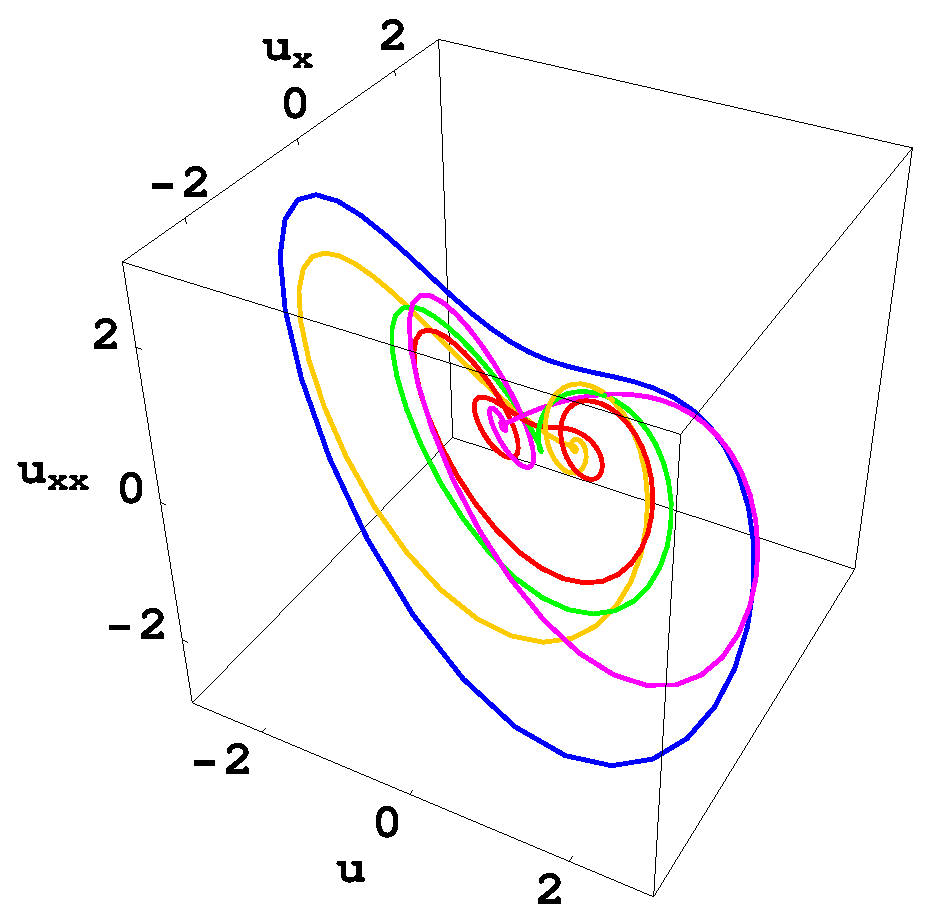
\includegraphics[width=0.35\textwidth, clip=true]{figs/equilSpatial.eps}
%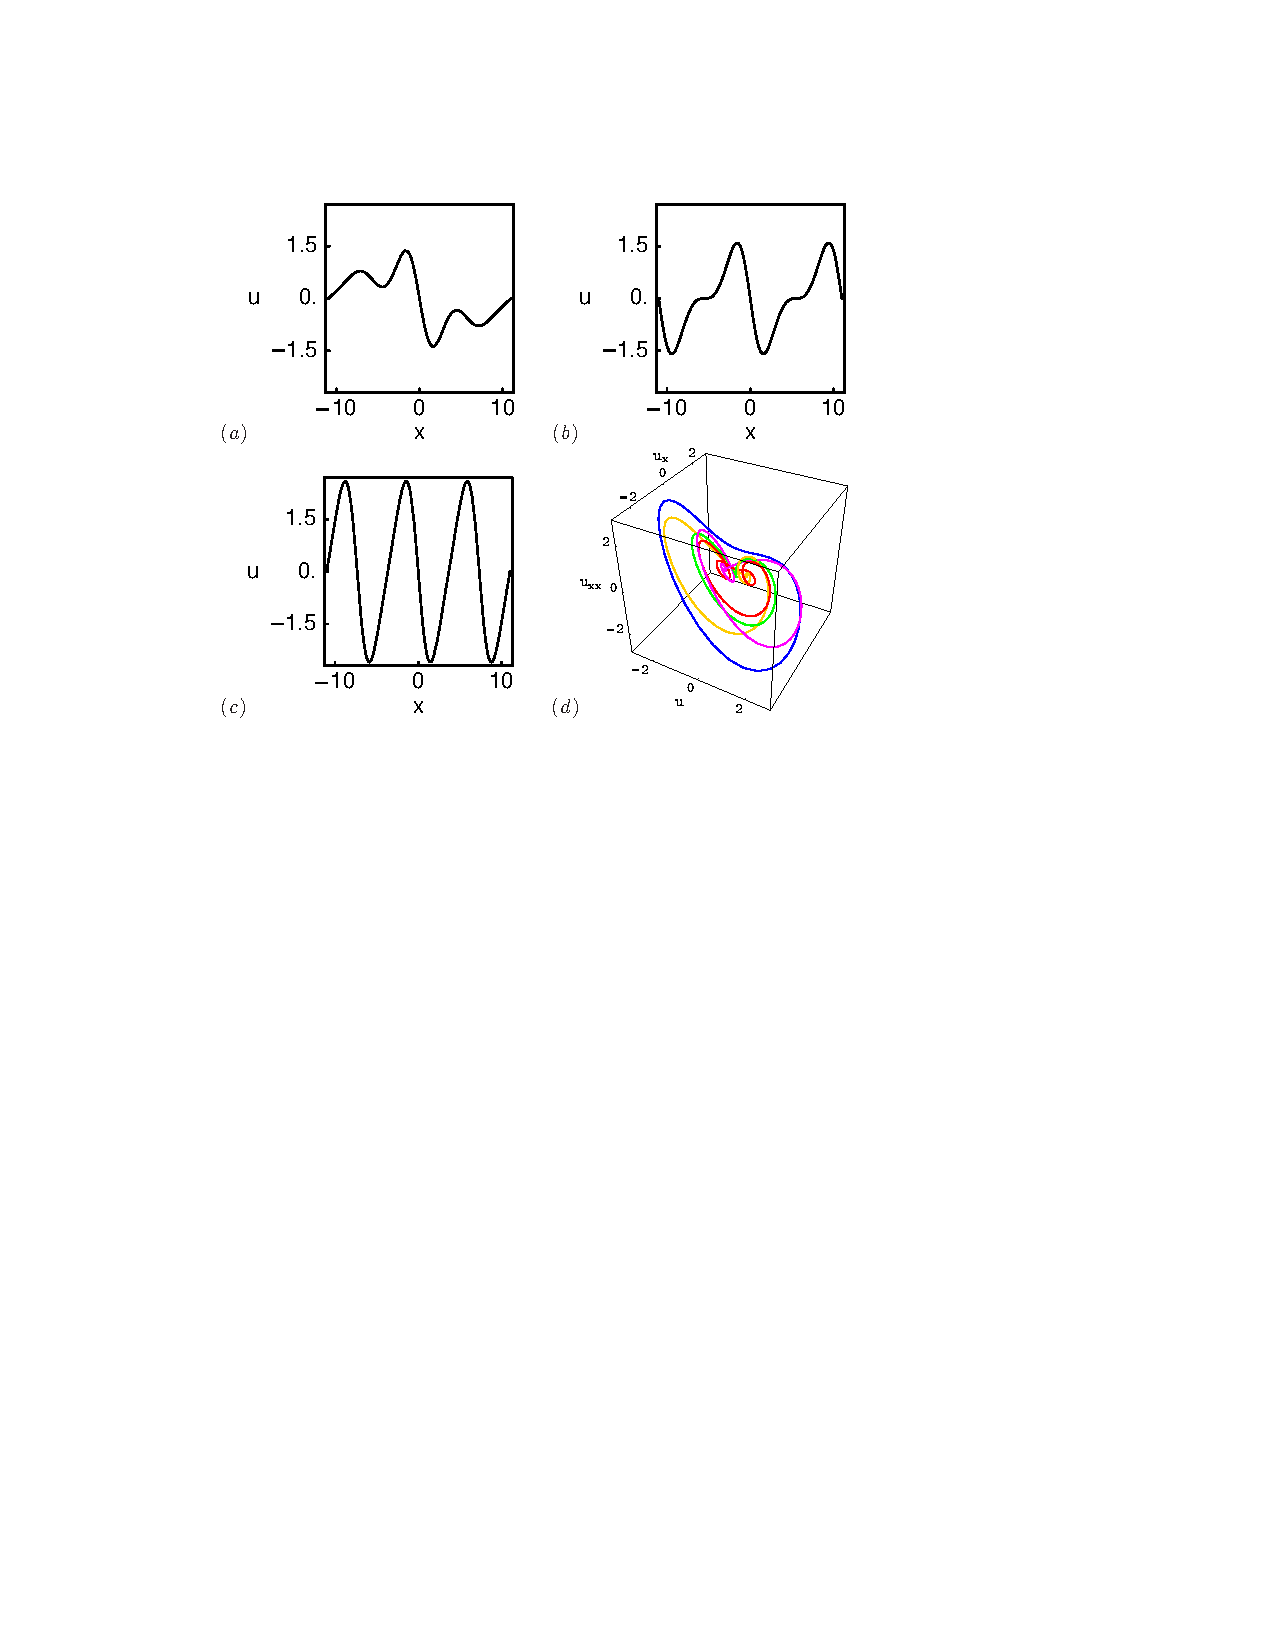
\includegraphics[width=0.95\textwidth]{SCD07fig5-1}
%\end{center}
%\caption{
%(a) \EQV{1}, (b) \EQV{2}, and (c)
%\EQV{3} \eqva. The \EQV{0} \eqv\ is the $u(x)=0$ solution.
%(d) $(u,u_x,u_{xx})$ representation
%of (red) \EQV{1}, (green) \EQV{2},  (blue) \EQV{3} \eqva,
%(purple) \REQV{+}{1},  and (orange) \REQV{-}{1} \reqva.
%$L=22$ system size.
%From Cvitanovi{\'c}, Davidchack and Siminos\rf{SCD07}.
%    }
%\label{f:KS22Equil}
%\end{figure}
%%%%%%%%%%%%%%%%%%%%%%%%%%%%%%%%%%%%%%%%%%%%%%%%%%%%%%%%%%%%%%%%%

\PCpost{2016-07-05}{
\refFig{fig:ppo1rpo1} from
Cvitanovi{\'c}, Davidchack and Siminos\rf{SCD07} gives you some indication
of what are typical sizes of $(u,u_x,u_{xx})$ for the $L=22$ spatial domain.
    }

\MNGpost{2016-07-06}{

\begin{description}

\item[BurakTalks]
Burak believes that the easiest way for me to pick up a spurious divergence is there is someplace, (most likely calculating the nonlinear term via pseudospectral method) where the normalizations of fft and ifft are incorrect.

In order to verify this, he suggested calculating the nonlinear term via both methods in \refeq{e-KScp}, i.e. a convolution sum and the other via the pseudo spectral method. The following is how I formulated \texttt{convolutionsum.m} for future reference. \\
\end{description}

Step Zero: Original ordering of Fourier modes ($N=2^p$), mode numbers range from $-N/2$ to $N/2-1$ in increments of 1, based on \texttt{fft} function in MATLAB

\begin{tabular}{c || c | c | c | c | c | c | c | c | c }
\hline
 Mode-numbered ordering of $\Fu^{(0)}$:
 & -N/2 & -N/2+1 & ... & -1 & 0 & 1 & ... & N/2-1  & N/2-1 \\ \hline
 Mode-Numbered Ordering of $\Fu^{(1)}$:
  & -N/2 & -N/2+1 & ... & -1 & 0 & 1 & ... & N/2-1  & N/2-1 \\ \hline
\end{tabular}

Step One: Cyclically permute $\Fu^{(0)}$ by $k-1$, reverse the ordering of $\Fu^{(1)}$, (Note: extra shift by 1 to get  into the right position due to reversing $\Fu^{(1)})$

\begin{tabular}{c || c | c | c | c | c | c | c | c | c }
\hline
 Mode-numbered o of $\Fu^{(0)}$:
 & N/2+k+1 & ... & k-2 & k-1 & k & k+1 & ... & N/2+k-1  & N/2+k \\ \hline
 Mode-numbered ordering of $\Fu^{(1)}$:
 & N/2-1 & ... & 2 & 1 & 0 & -1 & ... & -N/2+1 & -N/2 \\ \hline
 \end{tabular}

Final Step: Element-wise multiplication and summation of allowed combinations

Depending on whether we shift to the right($k<0$) or left($k\geq0$), the admissible combinations to the convolution sum are either the last $N-k$ elements (for $k<0$) or the first $N-k$ elements(for $k\geq0$). The admissability is a condition that arises from truncating the infinite sum to a sum from $-N/2$ to $N/2-1$


Although Burak predicted that I would need to multiply by a factor of $1/N$ in order to get my pseudo-spectral calculation to agree with the convolution sum calculation, I found the terrifying result that they matched when I multiplied the pseudo-spectral calculation by $N$, which would cause my equations to be even more unpredictable and has me questioning all of the different FFT's and IFFT's normalizations in my code.

\begin{description}
\item[XiongTalks]
Asked Xiong about how the spatial Fourier mode data produced by \texttt{ksint.m} is normalized and the correct procedure to acquire the correct amplitudes for $u(x_0,t)$ and its derivatives. He pointed me in the direction of \texttt{siminos/lyapunov/blog.pdf} which even though he claims is normalized unconventionally, I believe it fits with the MATLAB convention of including $1/N$ with the inverse FFT. This is a problem because this is what lead to the small values of $u(x_0,t)$ in the first place, more reasonable values (relative to the scale of figures in \refref{SCD07}).

\item[KSspaceint]
Still trying to find what I'm missing when it comes to whether the reason for numerical instability in my code is due to Fourier transform normalizations, the integration method I'm using, etc. Compared initial and final values produced by time integration of \texttt{ksint.m} of spatial Fourier modes, and the corresponding values of $u(x_0,0)$ and $u(x_0,20.5058)$ and found $u(x_0,0) - u(x_0,20.5058) \approx 10^{-9}$ for $x_0 = 1.375$ (point 2 out of 32 on spatial grid). I found this value of $x_0$ to yield somewhat smoother results than $x_0 = 11$, that's the reason for the change.

\end{description}
}

\PCpost{2016-07-08}{
When you write ``20.5058'' you mean not 20.5058, but $T= 2\,T_{\PPO{10.2}}$ to all
11 digits (or however many Xiong gives you) of precision, not a 6-digit number, right?
    }

\MNGpost{2016-07-07}{
% \color{red}
Still trying to figure out why the temporal Fourier modes do not drop off exponentially, as I believe this is one of the factors for the numerical instability I am faced with. Like I mentioned in my previous post, the order of the difference between the initial value $u(x_0,0)$ and $u(x_0,20.5058)$ for $x_0=1.375$ is $\approx 10^-9$, just to make sure this small discrepancy wasn't the problem, I forced the initial value and final value to be identical but this yielded no fruitful results.

I have been scouring documentation and testing new editions of my code \texttt{timeperiodic.m}. I tried to see if varying the amount of steps and amounts of temporal modes affected the amplitudes in a beneficial way but they did not.
%
%The only idea left to me is that maybe there is too much precision on the Fourier coefficients so that when I apply MATLAB's FFT it's picking up on modes that should normally not be present. I don't know if this claim makes sense to be quite honest. I take a time-periodic strip, apply an FFT (usually with the same number of modes as the number of data points in the strip for convenience), and get Fourier coefficients whose amplitudes level out at $\approx 10^{-4}$. Will try the numerical precision idea tomorrow.
%
%Edit: Realized that this was fatigue driven nonsense.
}

\MNGpost{2016-07-07}{
From Xiong's blog in {\em siminos/lyapunov/blog.pdf} eq.~(7.97) (label
{xfft2}): he seems to show that when converting from a convolution sum
of continuous Fourier modes, as in \refeq{e-KScp}, to a discrete
Fourier transform representation, there is an additional factor of
$1/N$ (N = number of modes) that I hadn't accounted for. The importance
behind this is that I believe this factor cancels the multiplication of
the pseudospectral term by $N$ that Burak and I had discussed, which
incidentally was creating bad results.
\\
{\bf Edited 2016-07-08}
\\
Another development: I was not defining the
frequencies for temporal Fourier modes correctly.
For continuous Fourier transforms, i.e. $\omega_k = 2\pi  k / T$, but for the
discrete transforms $w_k = 2\pi  k / N_t$ , where $N_t$ is the number of
data points input into the FFT.

This did not fix the code completely, but when I had, by accident, input
$w_k = 2\pi  k / T N_t$, I got somewhat stable (able to integrate from
$x=0$ to $x \approx 40$) results; will include a figure later. I believe
I am close to meaningful results.
}

\item[2016-07-08 Xiong]
Discrete FFT in matlab is
\[
  a_k = \sum^{N-1}_0 u(x_n) e^{-iq_kx_n} \,,\quad
  u(x_n) = \frac{1}{N} \sum_{k=0}^{N-1}a_k e^{iq_kx_n}
\]
But we are using
\[
  a_k = \frac{1}{N} \sum^{N-1}_0 u(x_n) e^{-iq_kx_n} \,,\quad
  u(x_n) = \sum_{k=0}^{N-1}a_k e^{iq_kx_n}
\]
So the normalization is different. ksint.m uses the C++ implementation of
\texttt{siminos/matlab/ruslan/ksfmetd2.m}. In this file, you can find the
nonlinear term coefficient is $g = 0.5i\,k\,N$, not $0.5i\,k$. This is how
Ruslan took care of the normalization difference. If you follow this
rule, your code should be fine. Embarrassingly, I forgot this difference
when producing \reffig{fig:ppo1rpo1}, and Predrag did not catch error in
time, so the wrong scale is in the published Ding and
Cvitanovi{\'c}\rf{DingCvit14}. The scale in \reffig{fig:ppo1rpo1} is
about 0.03. Multiplying it with $64$ (I use 64 modes in \refref{DingCvit14}),
you should get the scale in \reffig{SCD07f:KS22Equil}. %\reffig{f:KS22Equil}.

\PCpost{2016-07-09}{to Xiong:
Wow, that's painful - is it too late to fix \reffig{fig:ppo1rpo1} in Ding
and Cvitanovi{\'c}\rf{DingCvit14}? The paper is not on line yet. And can
you fix this in all current codes that you are using for \KS\ \PoincSec\ calculations, so this error does not seep into the coming \KS\
symbolic dynamics paper?
}

\begin{figure}
    \centering
(a) 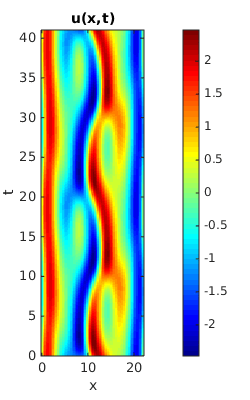
\includegraphics[width=0.35\textwidth,height=0.7\textwidth]{MNGppo1timeint}
~~~
(b) 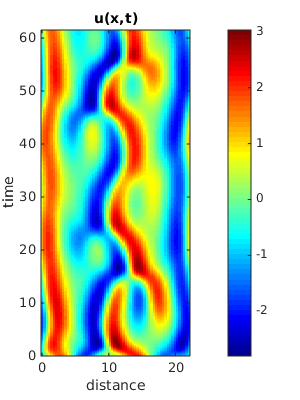
\includegraphics[width=0.35\textwidth,height=0.7\textwidth]{MNGode23stimeint}
    \caption{\label{fig:MNGtimeintL22}
    \Ppo\ $\PPO{10.2}$ of $L=22$ system integrated over
    (a) $t\in[0,
    4\,\period{\PPO{10.2}}]$ in order to compare to \reffig{fig:ppo1rpo1}.
    Produced by Kassam and Trefethen\rf{ks05com} \texttt{ksint.m}, but
    now correctly scaled, following Xiong.
    (b) $t=[0, 6\,T_{\PPO{10.2}}]$. Produced by MATLAB function
    \texttt{ode23s}.
    }
\end{figure}


\MNGpost{2016-07-09}{
Results from \refref{DingCvit14} reproduced in \reffig{fig:MNGtimeintL22}\,(a).
Vertical line from this data is used as initial condition for
space-integration.  Still can't get numerically stable results after more
testing and editing.

According to
\HREF{https://en.wikipedia.org/wiki/Discrete-time_Fourier_transform}
{Wikipedia} {\em Discrete-time Fourier transform},
the correct formulation for the frequencies is
\beq
\omega_k = \frac{2\pi k}{N T}
\ee{MNGdscrFreq}
($N$ is the number of modes).
\MNG{}{Edited the 2016-07-09 post to abide by this.}
    }

\PCpost{2016-07-09}{
Your code is an integrator. A suggestion, for testing purposes:

Why don't you test it as a \emph{time integrator} (instead of Kassam and
Trefethen\rf{ks05com} code - your code should be good enough for short
times integrations), start with Xiong's $u(x,0)_{\PPO{10.2}}$, integrate
\KS\ to $u(x,2\period{})_{\PPO{10.2}}$, see how well you reproduce
\reffig{fig:MNGtimeintL22}\,(a). When that works, return back to testing it as
an integrator in \emph{space}.
    }

\MNGpost{2016-07-11}{
%\color{red}
Realized after more testing that the stiffness of equations \refeq{e-ksX}
was not being addressed by the integrator I was implementing. I used
MATLAB integrator  \texttt{ode23s} to test time integration and produced
\reffig{fig:MNGtimeintL22}\,(b). As anyone can see this does not reproduce results
from \refref{DingCvit14}. Even with that in mind, I attempted to apply
\texttt{ode23s} to spatial integration and was left waiting for code to
compile that never completed. I now beginning to believe that in order to
get quick and accurate results from integration of these stiff PDE's that
I will have to adapt a different scheme for my code, possibly the code
from Kassam and Trefethen\rf{ks05com} in order to properly integrate.
This would involve using Chebyshev Differentiation Matrices as mentioned
in Kassam and Trefethen\rf{ks05com} or a similar method to represent the
linear terms because I don't believe the linear part of the equation can
be represented by a diagonal matrix.
}

\PCpost{2016-07-12}{
At least visually, the two integrators in \reffig{fig:MNGtimeintL22}
agree pretty well. Have you maybe committed the wrong
\reffig{fig:MNGtimeintL22}\,(b)? If not, why don't you show us the plot
of the spatial integrator, if not for $L=22$, at least for $x\in\{0,1\}$
with very small space-step integration, so we can see that you are
starting with $u(0,t)$ that agrees with \reffig{fig:ppo1rpo1}.

At this time, it is more important to get qualitatively right space
integration. We can worry about improving the integrator later. Perhaps
it is not the problem of a numerical integrator. Our starting
\refeq{e-FksX} might be wrong in some deep and profound way...
    }

\item[2016-07-12 Xiong to Matt]
\texttt{ode23s} has options to set the accuracy of each integration
step, and you can print out the integration statics. This implicit
integrator has order 2, so you should not expect your result to be
very accurate. Other choice maybe \texttt{ode15s}.

You observed that \texttt{ode23s} halted forever for spatial integration.
It means that it is reducing the time step to an extremely small
value so as to match the local error tolerance. Probably, you can
increase this tolerance to get a qualitative picture. As you know,
implicit scheme like \texttt{ode23s} are always stable.


\PCpost{2016-07-05}{
I order to match up with our temporal evolution of \KS\ plots,
in $u(x,t)$ color-coded plots always plot the spatial $x$ coordinate
along the $x$-axis, increasing from the left to the right, and the
temporal $t$ coordinate along the $y$ axis, increasing from $t=0$
upwards. Label axes $x$ and $t$, not using words. Try to use the same
units, \ie, if one plot is time-periodic on $T=7$ and the other on
$T=14$, the strip representing the second plot should be twice as wide.

Makes it easier to eyeball different plots...
    }

\PCpost{2016-07-08}{
In preparing the initial condition for the space integration, when you
write ``20.5058'' you mean not the 6-digit number 20.5058, but $T=
2\,T_{\PPO{10.2}}$ to all 11 digits (or however many Xiong gives you) of
precision, right?
    }

\MNGpost{2016-07-13}{

\begin{description}
\item[Comments]
I am indeed using $T=2\,T_{\PPO{10.2}}$.

On the comments about the graphical conventions, I will adhere to this from now on; I think it will be easier to scale in LaTeX, rather than scaling the MATLAB output as I have been doing.


Found another resource \HREF{http://blogs.mathworks.com/steve/2010/03/15/the-dft-and-the-dtft/}{MATLAB forum} that uses $\omega_k = \frac{2\,\pi\,k}{N}$ for the frequencies. Using this in latest formulation.

\item[MattToXiong]
I think I have experienced what you have mentioned in the past, in regards to error tolerances; when my code was incorrect it was reducing the step size to
$\Delta x \approx 10^{-14}$. I will definitely look into the error tolerances tomorrow.

\item[QuestionForBurak]
I think I might have misinterpreted what Burak wrote down some time ago, in reference to his statement:

$\epsilon u^{(3)}_{tt}$ to the RHS of the first equation in \refeq{e-ksX}, which would show up as $- \epsilon \omega_k^2 \Fu_k$ in Fourier space.

Does this mean that I should have a term that looks like $- \epsilon \omega_k^2 \Fu^{(3)}_{k}$? or $- \epsilon \omega_k^2 \Fu^{(0)}_{k}$? (Note: The only difference is the superscripts) I have been using $- \epsilon \omega_k^2 \Fu^{(3)}_{k}$ and now I am full of doubts.

%\item[KSspaceint]
%I was going to upload more new figures but now I think it's slightly too premature, I think it would be better to get an answer Burak and apply a little bit more testing before uploading.

\end{description}
    }

\NBBpost{2016-07-13}{to Matt:
Your original interpretation was right, I corrected my previous post.
}

\begin{figure}[ht]
  \begin{minipage}[height=.40\textheight]{.32\textwidth}
    \centering
    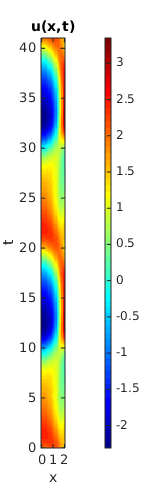
\includegraphics[width=\textwidth,height=.40\textheight]{MNGxint2altwkep1}
    \small{\texttt{$\omega_k = \frac{2 \pi k}{N\,T}$ $e=0.1$}}
  \end{minipage}
  \begin{minipage}[height=.40\textheight]{.32\textwidth}
    \centering
    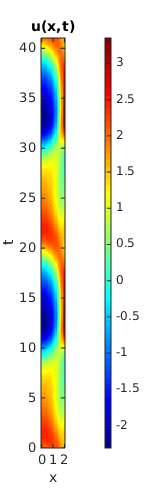
\includegraphics[width=\textwidth,height=.40\textheight]{MNGxint2e0}
    \small{\texttt{$\omega_k = \frac{2 \pi k}{N}$ $e=0$}}
  \end{minipage}
  \begin{minipage}[height=.40\textheight]{.32\textwidth}
    \centering
    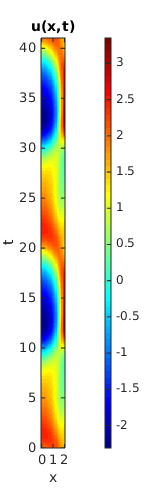
\includegraphics[width=\textwidth,height=.40\textheight]{MNGxint2ep1}
    \small{\texttt{$\omega_k = \frac{2 \pi k}{N}$ $e=0.1$}}
  \end{minipage}
  \caption{
  Spatial integration of initial temporal strip of $u_{\PPO{10.2}}$,
  ($T=4\,T_{\PPO{10.2}}$) for $x = [0,2]$ with varying the conflicting
  definitions for the frequencies $\omega_k$ and varying the artificial
  diffusion constant $e$.
  I believe that the reason why there is no difference between
%\PCpost{2016-07-23}{
  the first and second panel is
  because both were poorly formulated due to the misstep I had with the
  frequencies mentioned in my post of 2016-07-21.
  I also changed the $- i \omega_k \Fu^{(0)}_k$ to both $i \omega_k
  \Fu^{(0)}_k$ and  $\omega_k \Fu^{(0)}_k$, with no effect on the spatial
  integrations displayed here. In retrospect, the plots displayed here
  are quite meaningless.
  }
  \label{fig:MNGxint2}
\end{figure}

\begin{figure}[h]
  \begin{minipage}[height=.40\textheight]{.32\textwidth}
    \centering
    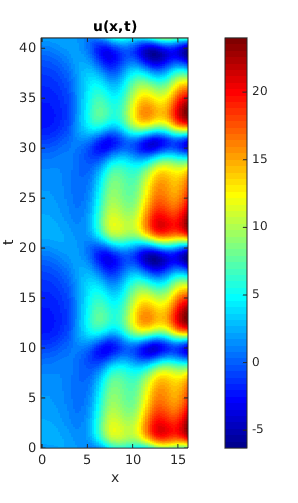
\includegraphics[width=\textwidth,height=.40\textheight]{MNGxint16altwkep1}
    \small{\texttt{$\omega_k = \frac{2 \pi k}{N\,T}$ $e=0.1$}}
  \end{minipage}
  \begin{minipage}[height=.40\textheight]{.32\textwidth}
    \centering
    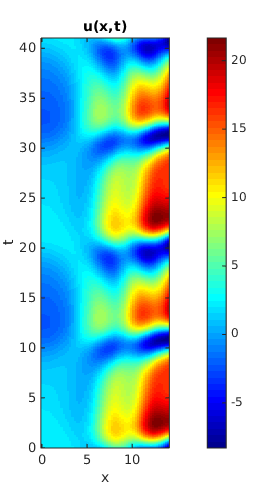
\includegraphics[width=\textwidth,height=.40\textheight]{MNGxint16e0}
    \small{\texttt{$\omega_k = \frac{2 \pi k}{N}$ $e=0$}}
  \end{minipage}
  \begin{minipage}[height=.40\textheight]{.32\textwidth}
    \centering
    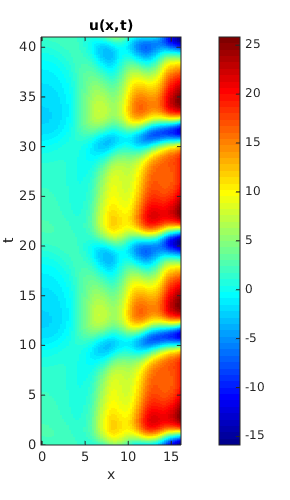
\includegraphics[width=\textwidth,height=.40\textheight]{MNGxint16ep1}
    \small{\texttt{$\omega_k = \frac{2 \pi k}{N}$ $e=0.1$}}
  \end{minipage}
  \caption{
  Spatial integration of initial temporal strip of $u_{\PPO{10.2}}$, ($T=4\,T_{\PPO{10.2}}$) for $x = [0,16]$
  with varying the conflicting definitions for the frequencies $\omega_k$ and varying the artificial diffusion constant $e$}
  \label{fig:MNGxint16}
\end{figure}

\begin{figure}[h]
  \begin{minipage}[height=.40\textheight]{.32\textwidth}
    \centering
    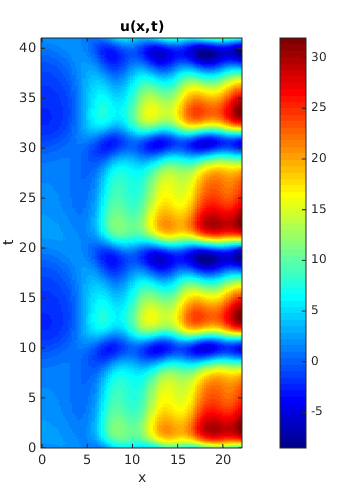
\includegraphics[width=\textwidth,height=.40\textheight]{MNGxint22altwkep1}
    \small{\texttt{$\omega_k = \frac{2 \pi k}{N\,T}$ $e=0.1$}}
  \end{minipage}
  \begin{minipage}[height=.40\textheight]{.32\textwidth}
    \centering
    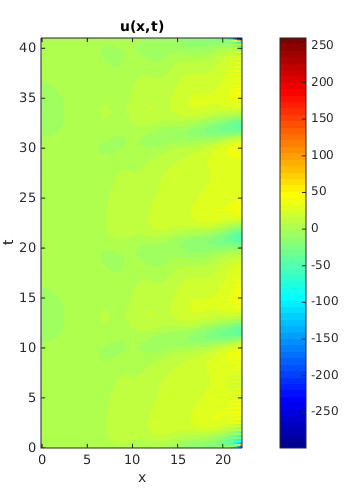
\includegraphics[width=\textwidth,height=.40\textheight]{MNGxint22e0}
    \small{\texttt{$\omega_k = \frac{2 \pi k}{N}$ $e=0$}}
  \end{minipage}
  \begin{minipage}[height=.25\textheight]{.32\textwidth}
    \centering
    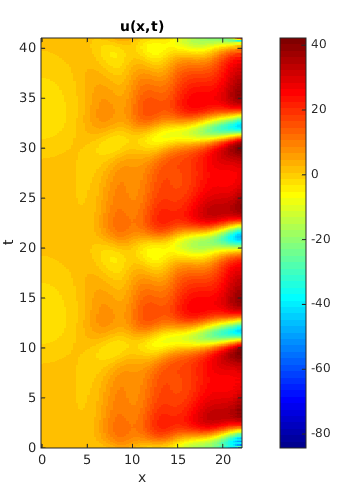
\includegraphics[width=\textwidth,height=.40\textheight]{MNGxint22ep1}
    \small{\texttt{$\omega_k = \frac{2 \pi k}{N}$ $e=0.1$}}
  \end{minipage}
   \caption{
  Spatial integration of initial temporal strip of $u_{\PPO{10.2}}$, ($T=4\,T_{\PPO{10.2}}$) for $x = [0,22]$
  with varying the conflicting definitions for the frequencies $\omega_k$ and varying the artificial diffusion constant $e$.
  }
  \label{fig:MNGxint22}
\end{figure}

\begin{figure}[h]
    \centering
  \begin{minipage}[height=.40\textheight]{.32\textwidth}
    \centering
    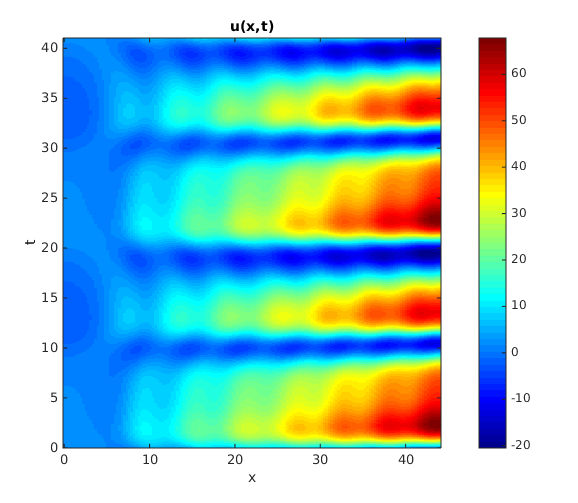
\includegraphics[width=\textwidth,height=.40\textheight]{MNGxint44altwkep1}
    \small{\texttt{$\omega_k = \frac{2 \pi k}{N\,T}$ $e=0.1$}}
  \end{minipage}
    \caption{
    Spatial integration of initial temporal strip of $u_{\PPO{10.2}}$,
    ($T=4\,T_{\PPO{10.2}}$) for $x = [0,44]$.}
    \label{fig:MNGxint44}
\end{figure}


\MNGpost{2016-07-13}{

I have included plots \reffig{fig:MNGxint2}, \ref{fig:MNGxint16}, \ref{fig:MNGxint22}, and \ref{fig:MNGxint44} of spatial integration of \refeq{e-FksX} using my code \texttt{timeperiodic.m} and \texttt{velocityfunction} (which I really should rename).

I varied the definitions of $\omega_k$ because I still find conflicting
sources. I believe \reffig{fig:MNGxint44} is evidence showing that indeed
$\omega_k = \frac{2 \pi k}{N\,T}$ is the correct formulation because I could
not produce similar results for integration over $x = [0,44]$ with the
alternative definition: $\omega_k = \frac{2 \pi k}{N}$.

The specific value of $e=0.1$ was initially random. After some testing, it seemed to have no effect for $\omega_k = \frac{2 \pi k}{N\,T}$ plots. Its effect on the $\omega_k = \frac{2 \pi k}{N}$ plots was such that for $e \leq 0.05$ the values of $u(x,t)$ would diverge faster. For values $e \geq 0.1$ there were diminishing returns, as the results for $e = 1$, $e = 10$ and $e = 100$ were almost identical.

}


\begin{figure}[ht]
  \begin{minipage}[height=.40\textheight]{.32\textwidth}
    \centering \small{\texttt{(a)}}
    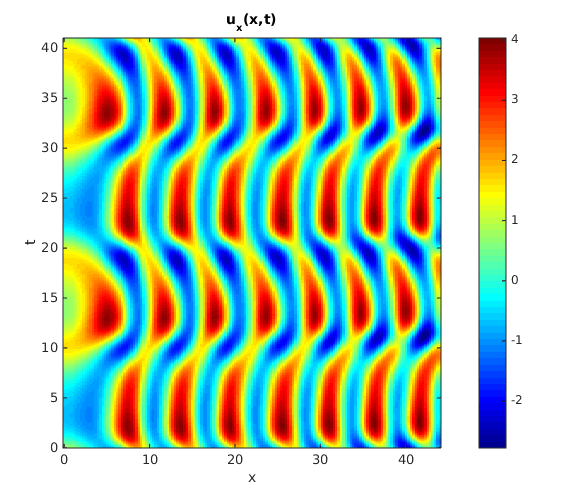
\includegraphics[width=\textwidth,height=.40\textheight]{MNGduxint44ep1}
    \small{\texttt{$\omega_k = \frac{2 \pi k}{N\,T}$ $e=0.1$}}
  \end{minipage}
  \begin{minipage}[height=.40\textheight]{.32\textwidth}
    \centering \small{\texttt{(b)}}
    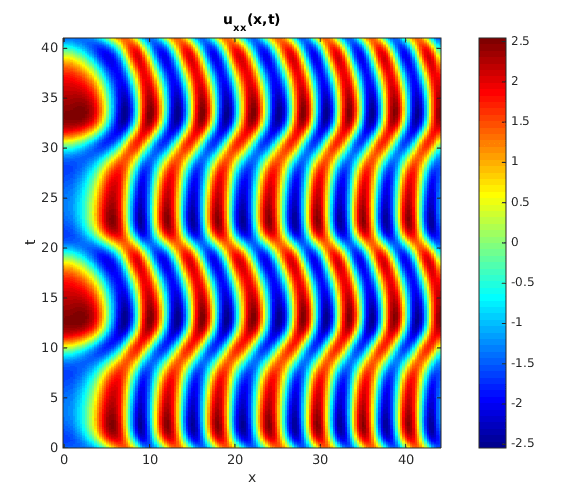
\includegraphics[width=\textwidth,height=.40\textheight]{MNGdduxint44ep1}
    \small{\texttt{$\omega_k = \frac{2 \pi k}{N\,T}$ $e=0.1$}}
  \end{minipage}
  \begin{minipage}[height=.25\textheight]{.32\textwidth}
    \centering \small{\texttt{(c)}}
    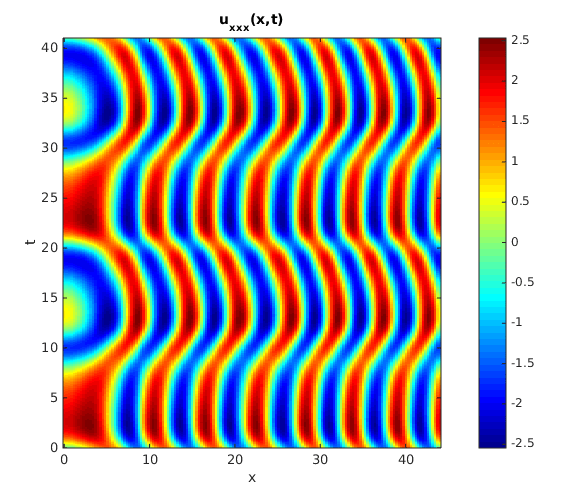
\includegraphics[width=\textwidth,height=.40\textheight]{MNGddduxint44ep1}
    \small{\texttt{$\omega_k = \frac{2 \pi k}{N\,T}$ $e=0.1$}}
  \end{minipage}
   \caption{
  Spatial integration of initial temporal strip derivatives of
  $u_{\PPO{10.2}}$, ($T=4\,T_{\PPO{10.2}}$) for $x = [0,44]$.
  (a) $u_{x}(x,t)$, (b) $u_{xx}(x,t)$, and (c) $u_{xxx}(x,t)$.
  In retrospect, the plots here are not correct, due to the confusion I
  was having with frequencies. In the spirit of the experimenter's
  notebook, we keep here the record of all results, good and bad.
  }
  \label{fig:MNGxint44deriv}
\end{figure}

\MNGpost{2016-7-14}{
%\color{red}
Spent today with more testing and investigation into why the values of
$u(x,t)$ seem to increase as the integration range is increased. In
\reffig{fig:MNGxint44} I show that after some initial length $x$ the
derivatives appear periodic. I am hesitant to say there is ``transient"
behavior because this happens in a finite spatial interval, not time, but the
fact remains that the spatial derivatives
$u_x(x,t)$, $u_{xx}(x,t)$ and $u_{xxx}(x,t)$  seem to be well-behaved while
$u(x,t)$ itself is not.

I believe this is due to the first equation of \refeq{e-FksX} being
dominated by the term $\Fu^{(2)}_{k}$.
}

\PCpost{2016-07-22}{
According to \refeq{e-Fseries} the correct definition for a continuous
time Fourier transform is is $\omega_k=2\pi k/\period{}$. You say that
\reffig{fig:MNGxint44} shows that $\omega_k=\frac{2\pi k}{N\,T}$ is the
correct definition. Maybe you can add some further text to the
discretization approximation \refeq{e-FdscrApprx} and show that the
continuous time Fourier transform \refeq{e-Fseries} indeed leads to
\refeq{MNGdscrFreq}.
\\{\bf Matt 2016-07-25}
Because $\omega_k$ is coming from term $- u^{(0)}_{\zeit}$ when written
in terms of continuous time Fourier modes, I believe the correct
definition to use is the expression $\omega_k = \frac{2 \pi k}{T}$. It
is then that the terms $\Fu_k$ are replaced by their discretized
versions, namely \\
$\Fu_k = \frac{1}{N} \sum_{n=0}^{N-1} u(t_n) e^{-i
2 \pi n k / N} = \frac{1}{N} \mathcal{F} \{ u (t_n) \}$ \.
Unless there is
something I didn't understand from what Burak has told me (and written
in \refsect{sect:FTnormal}), I believe I have done this correctly.
        }

\NBBpost{2016-07-13}{
In \refsect{sect:FTnormal} I go through the derivation of \refeq{e-FksX}
in order to clarify all possible normalization related issues in Fourier
transforms. Please go through \refsect{sect:FTnormal}, make sure each
step is correct, both on paper and in your code.
}

\MNGpost{2016-07-18}{
Went through calculations as Burak requested. I was in agreement with the results but
would like to hear whether there is a reason for the pseudospectral term to be written
as $\frac{1}{N} \mathcal{F} \{ u^{(0)} u^{(1)} \}$ versus an expression that is completely
in terms of Fourier modes. There might be a subtlety I'm not picking up on, but my derivations
implied that it could be written instead as a convolution between $\Fu^{(0)}_{k}$ and $\Fu^{(1)}_{k}$.
The reason why I would want to keep everything in terms of Fourier modes is because I feel like it
would make the integrator more efficiently.
\\{\bf Predrag  2016-07-23} I think the general strategy of
pseudospectral codes is to evaluate nonlinear terms in the configuration
space, then do integration stepping in the Fourier representation.
\\{\bf Xiong 2016-07-24 }
Using $\frac{1}{N} \mathcal{F} \{ u^{(0)}
u^{(1)} \}$ instead an expansion in Fourier modes because of their
different computational complexity: $O(N\log N)$ versus $O(N^2)$.

Thanks a lot for the help Burak! I really do appreciate it.
}

\begin{figure}[h]
\centering
  \begin{minipage}[height=.40\textheight]{.32\textwidth}
    \centering
    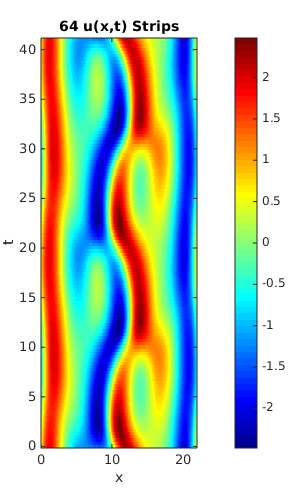
\includegraphics[width=\textwidth,height=.40\textheight]{MNGcompxint22}
    \small{\texttt{$\omega_k = \frac{2 \pi k}{T}$ $e=0.0001$}}
  \end{minipage}
\caption{
Spatial integration results for 64 time periodic strips
$T=4\,T_{\PPO{10.2}}$ from the time evolution of $\PPO{10.2}$ compiled
into one image. The time periodic strips were generated by Xiong's MATLAB
code \texttt{ksint.m}. The initial time periodic strips were integrated
over spatial intervals $[x_n, x_{n+1}]$ with $x_n = 22 \frac{n}{64}$, $n
= 0, ..., 63$.
        }
\label{fig:MNGcompxint}
\end{figure}

\MNGpost{2016-07-19}{
%\color{red}
I finished applying changes to my code that Burak helped me with.

After more testing and still having diverging results, but having seemingly good results for
small spatial integration $x \in [0,\approx 1]$ I decided that the best test for my code in its current state was to
glue a bunch of spatial integration results together and see if they agreed with the time-integrated results.
Specifically, there were a total of 64 strips integrated over intervals $[x_n, x_{n+1}]$ with
$x_n = 22 \frac{n}{64}$ , $n = 0 , ... , 63$ . The main integrator used was \texttt{ode15s}
from MATLAB, with step sizes of $\Delta x = 0.01375$ (each strip had 25 steps for the spatial integration).

The results look better than I expected because my code hasn't been able to produce results from a single
time periodic strip, integrated over $x = [0,22]$. Although I made a small mistake when producing this figure, it should not be the cause of
why it seems to be evolving backwards in time when compared to the time evolution of $\PPO{10.2}$ seen
in \reffig{fig:ppo1rpo1} from Ding and Cvitanovi{\'c}\rf{DingCvit14}.

Although it turned out better than expected, I'm unsure if these results are meaningful in the long run because
of the small spatial extent of each spatially integrated strip, they may not be large enough to truly demonstrate
spatial evolution; but I am still hopeful about the result.
}

\NBBpost{2016-07-20}{
\refFig{fig:MNGcompxint} looks nice and I think it is a meaningful test.
Although I can see a discontinuity around $x = L/2$, that is probably a minor
error. I wonder if you can reproduce this figure with $\epsilon = 0$; $10^{-4}$
is still very high. Moreover, if your spatial integration works for
$\Delta x \approx 1$, then why don't you use $22$ different strips rather than
$64$ so that we can see more clearly if something went wrong.

I had a quick look at your code to check one thing: When you are taking initial
time strip data from time-integration, I think you are taking an interval
$t = [0, 4 \period{}]$, including $t = 4 \period{}$, if this is the case, you
should change it to $t = [0, 4 \period{})$ excluding the final point in time,
see definitions of Fourier transforms above. I'm not sure how much change this
would cause but this might be the reason why \reffig{MNGinitialfourier} does
not drop off as it should, because including final point messes up the
smoothness.
}

\begin{figure}[h]
  \begin{minipage}[height=.20\textheight]{.25\textwidth}
    \centering \small{\texttt{(a)}}
    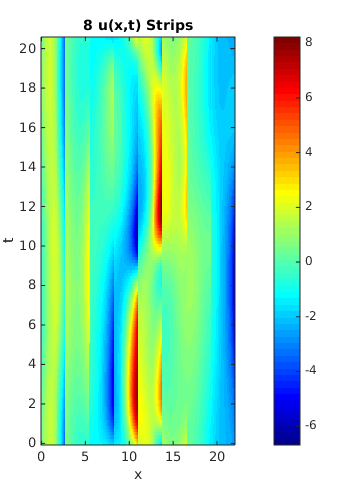
\includegraphics[width=\textwidth,height=.20\textheight]{MNGcomp8xint22}
  \end{minipage}
  \begin{minipage}[height=.20\textheight]{.25\textwidth}
    \centering \small{\texttt{(b)}}
    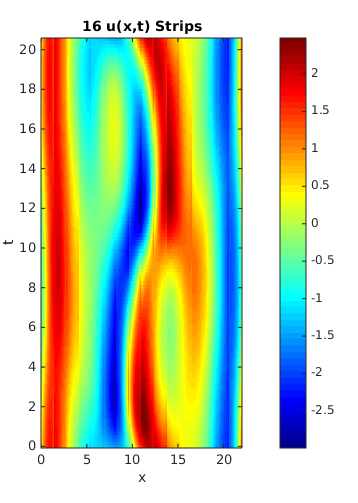
\includegraphics[width=\textwidth,height=.20\textheight]{MNGcomp16xint22}
  \end{minipage}
  \\
  \begin{minipage}[height=.20\textheight]{.25\textwidth}
    \centering \small{\texttt{(c)}}
    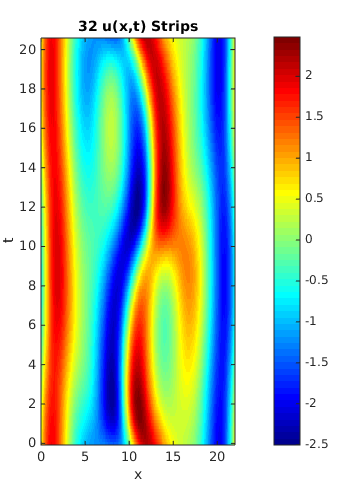
\includegraphics[width=\textwidth,height=.20\textheight]{MNGcomp32xint22}
  \end{minipage}
  \centering
  \begin{minipage}[height=.20\textheight]{.25\textwidth}
    \centering \small{\texttt{(d)}}
    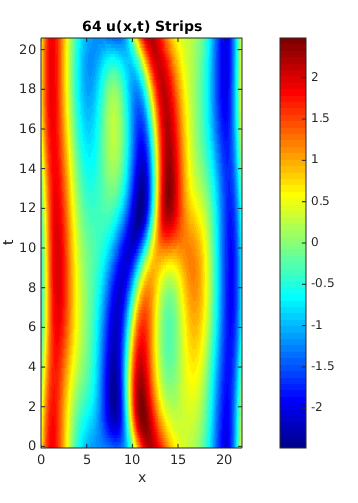
\includegraphics[width=\textwidth,height=.20\textheight]{MNGcomp64xint22}
  \end{minipage}
   \caption{
   Spatial integration $x=[0,22]$ with zero artificial diffusion ($e=0$).
   Initial conditions are time periodic strips $t = [0,
   2\,T_{\PPO{10.2}})$ provided by \texttt{ksint.m}. The number of
   integration strips, (i.e., the number of time-periodic initial
   conditions from \texttt{ksint.m} used for spatial integration)
   are: (a) 8, (b) 16, (c) 32, and (d) 64.
   }
  \label{fig:MNGcompxint2}
\end{figure}

\MNGpost{2016-07-20}{
\begin{description}
%\color{red}
\item[MattToBurak]

Fixed the the time interval to be $t = [0, 4\,T_{\PPO{10.2}})$ as opposed
to $t = [0, 4\,T_{\PPO{10.2}}]$, and set $e = 0$. Both had no effect on
the solutions. I believe that I just messed up the indices on the loop I
am running, which fixed the discontinuity that was apparent in
\reffig{fig:MNGcompxint}, and no longer in the respective figure, (d), in
\reffig{fig:MNGcompxint2}. The intricacies are hard to notice but I
attempted to keep them scaled the same as \reffig{fig:MNGcompxint}. The
qualitative behavior for 8 strips is wildly different from the others.
Although hard to see, there are a number of discontinuities for 16
strips, and the behavior for 32 and 64 seem identical.
\\
{\bf Predrag 2016-07-22} I interpret
  \reffig{fig:MNGcompxint2}\,(a) as indication that the spatial
  integration is not working, the remaining plots as indication that the
  spatial transient is longer than $L/16$ or so... Do you agree?
  \\
  {\bf Matt} I agree. It seems the best my code can do
in its current form is spatial integration to about $x \approx 1$ if
there are to be no discontinuities.

Based on Predrag's recommendation I changed the time interval from $t =
[0, 4\,T_{\PPO{10.2}})$ to $t = [0, 2\,T_{\PPO{10.2}})$ as it might help
the solutions be more stable.

\item[KSspaceint]
Attempted again to find the cause of the divergence by playing with
equations \refeq{e-FksX} by introducing scaling factors on the different
terms and proceeding with spatial integration. So far the only definitive
result is that making the nonlinear term larger makes the equations blow
up faster, which is not very surprising. I also changed the $- i \omega_k
\Fu^{(0)}_k$ to be both $i \omega_k \Fu^{(0)}_k$ and  $\omega_k
\Fu^{(0)}_k$ with no effect on the spatial integrations for
\reffig{fig:MNGcompxint2}. My main motivation was to try simple things
which could possibly have an effect. I thought the main problem was the
nonlinear term, but if I recall correctly I removed it from the equation
in an albeit ridiculous procedure, and I still had the divergence
problem. I'll verify this tomorrow because I'm having trouble recalling
if that's actually what I did, but I wanted to write it down to remind
myself.
\end{description}
}

\begin{figure}[ht]
  \begin{minipage}[height=.45\textheight]{.45\textwidth}
    \centering \small{\texttt{(a)}}
    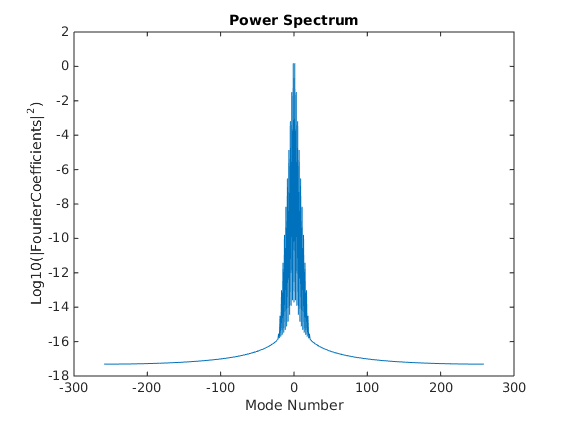
\includegraphics[width=\textwidth,height=.45\textheight]{MNGps1}
  \end{minipage}
  \begin{minipage}[height=.45\textheight]{.45\textwidth}
    \centering \small{\texttt{(b)}}
    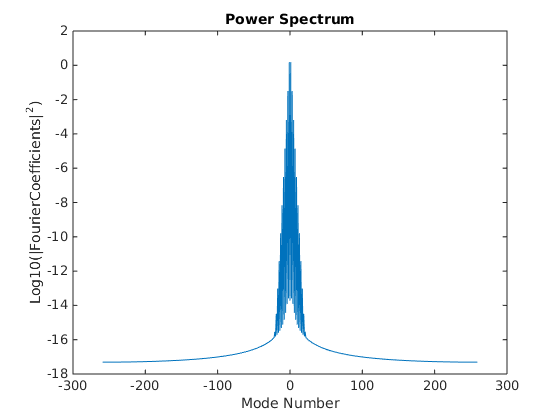
\includegraphics[width=\textwidth,height=.45\textheight]{MNGps2}
  \end{minipage}
   \caption{Double-sided power spectrum: $\log_{10}|\Fu^{(0)}_{k}|^2$ for initial time-periodic strips
   (a) $t = [0, 2\,T_{\PPO{10.2}}]$
   and (b) $t = [0, 2\,T_{\PPO{10.2}})$ where the number of modes is $N=520$}
  \label{fig:MNGFinit520}
\end{figure}

\begin{figure}[h]
  \begin{minipage}[height=.45\textheight]{.45\textwidth}
    \centering \small{\texttt{(a)}}
    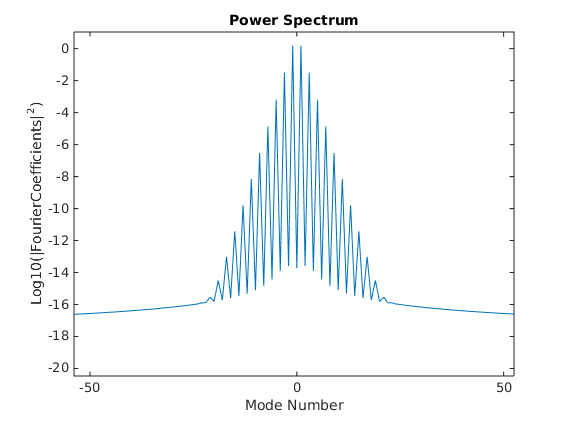
\includegraphics[width=\textwidth,height=.45\textheight]{MNGps3}
  \end{minipage}
  \begin{minipage}[height=.45\textheight]{.45\textwidth}
    \centering \small{\texttt{(b)}}
    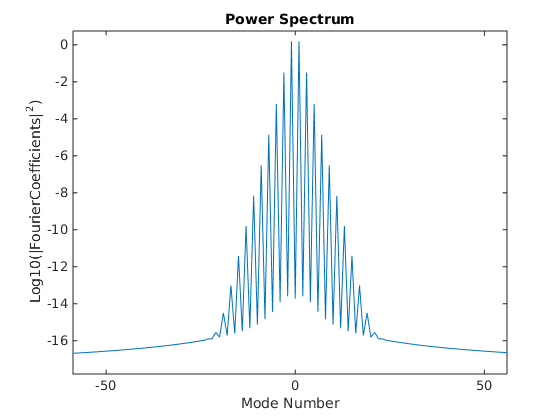
\includegraphics[width=\textwidth,height=.45\textheight]{MNGps4}
  \end{minipage}
   \caption{
   Double-sided power spectrum: $\log_{10}|\Fu^{(0)}_{k}|^2$ for initial time-periodic strips (a) $t \in [0, 2\,T_{\PPO{10.2}}]$
   and (b) $t \in [0, 2\,T_{\PPO{10.2}})$. This is the same as \reffig{fig:MNGFinit520} except zoomed in to show $\approx 100$ modes. \color{red} Note: The windowing
   is slightly off between the two as I did this by hand.
            }
  \label{fig:MNGFinit100}
\end{figure}

\begin{figure}[h]
  \begin{minipage}[height=.20\textheight]{.48\textwidth}
    \centering \small{\texttt{(a)}}
    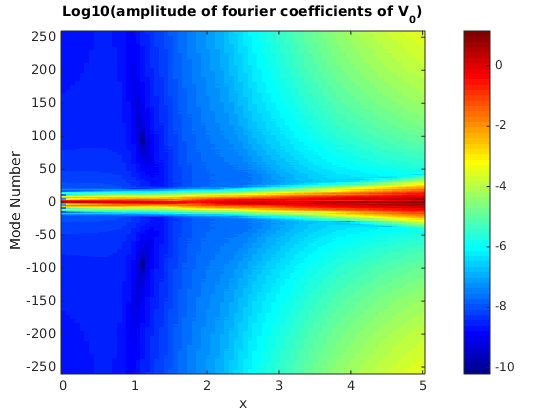
\includegraphics[width=\textwidth,height=.20\textheight]{MNGF0xint5}
  \end{minipage}
  \begin{minipage}[height=.20\textheight]{.48\textwidth}
    \centering \small{\texttt{(b)}}
    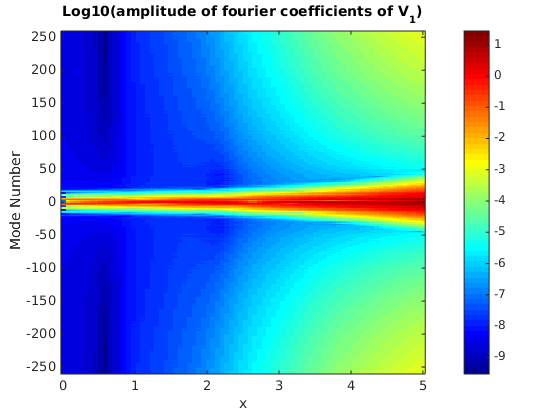
\includegraphics[width=\textwidth,height=.20\textheight]{MNGF1xint5}
  \end{minipage}
  \\
  \begin{minipage}[height=.20\textheight]{.48\textwidth}
    \centering \small{\texttt{(c)}}
    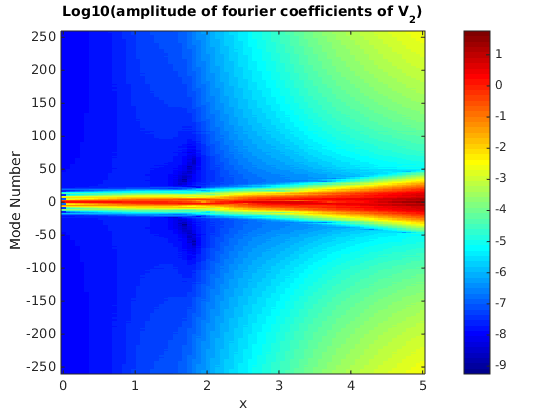
\includegraphics[width=\textwidth,height=.20\textheight]{MNGF2xint5}
  \end{minipage}
  \centering
  \begin{minipage}[height=.20\textheight]{.48\textwidth}
    \centering \small{\texttt{(d)}}
    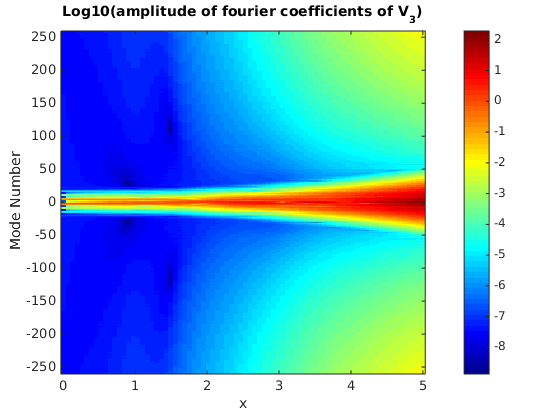
\includegraphics[width=\textwidth,height=.20\textheight]{MNGF3xint5}
  \end{minipage}
   \caption{
   Spatial integration $x=[0,5]$ of temporal Fourier mode amplitudes plotted on a
   $\log_{10}$ scale. Each vertical strip is a fast Fourier transform of a
   time periodic strip $t = [0, 2\,T_{\PPO{10.2}})$ provided by
   \texttt{ksint.m}.
   (a) $\Fu^{(0)}_{k}$, (b) $\Fu^{(1)}_{k}$,
   (c) $\Fu^{(2)}_{k}$, and (d) $\Fu^{(3)}_{k}$.
            }
  \label{fig:MNGFxint5}
\end{figure}

\MNGpost{2016-07-21}{:
%\color{red}
\begin{description}
\item[PowerSpectrumFigures]
The first set of figures in \reffig{fig:MNGFinit520} are the power spectra for initial time-periodic conditions for
$t = [0, 2\,T_{\PPO{10.2}}]$ and $t = [0, 2\,T_{\PPO{10.2}})$ in order to compare whether there are any differences.
Because the interesting details are hard to see, I've also included \reffig{fig:MNGFinit100} which are merely magnified
versions of \reffig{fig:MNGFinit520}. There seems to be no difference between the two, when taking my poor windowing into
consideration.

Some key things to note about the plots in \reffig{fig:MNGFxint5} is that
this is the power spectrum on a logarithmic scale,
$\log_{10}|\Fu^{(0)}_{k}|^2$, as opposed to the amplitude spectrum in
\reffig{MNGinitialfourier}. The other key difference is that I am using
the normalization convention $\Fu_k = \frac{1}{N} \mathcal{F} \{ u (t_n)
\}$. Previously I was dividing by N on application of the inverse FFT.

When the number of modes is smaller than the number of time steps, the
amplitudes are much larger in magnitude. When the number of modes is
taken to be greater than the number of time steps, the amplitudes
resemble the Fourier transform of a rectangular window function. The optimal
(smallest amplitudes) number of modes seems to be equal to the number of
time steps.

\item[FourierSpaceInt]
Also included in this blog post are plots of the spatially integrated
Fourier mode \emph{amplitudes}
    \PCedit{
$|\Fu^{(0)}_{k}|$,
           }
plotted on a $\log_{10}$ scale, in an attempt to see why the equations
are still unstable. I thought that this might be useful in identifying
any peculiar behavior, but all of the plots in \reffig{fig:MNGFxint5} are
very similar to each other. $\Fu^{(3)}_{k}$ seems to blow up first which
drags the rest $\Fu^{(0)}_{k}$, $\Fu^{(1)}_{k}$, $\Fu^{(2)}_{k}$, with
it. This interpretation is based on the scales included in the figures.
\end{description}
}

\PCpost{2016-07-23}{ %comment on \MNGpost{2016-07-21}{:
I do not understand the difference between (a) and (b) in
\reffig{fig:MNGFinit520} and \reffig{fig:MNGFinit100}. Presumably they
are time-power spectra for time-periodic $u(x_0,t)$  at different fixed
$x_0$?
    \\{\bf Matt} The difference in (a) and (b) is the
    \reffig{fig:MNGFinit520} and \reffig{fig:MNGFinit100} was based on
    Burak's recommendation to check and see whether having $t = [0, 4
    \period{}]$ vs. $t = [0, 4 \period{})$, (the latter being correct)
    had an impact on the amplitude spectrum / power spectrum.
    I was using MATLAB's absolute value feature $abs()$ so I'm certain
    they are being calculated the correct way.

Why are they oscillating wildly? Are you really looking at
complex amplitudes when you write $|\Fu^{(0)}_{k}|^2$, or are
you squaring the imaginary and real part separately? It looks like your
even modes mean something, and all odd modes are vanishing. That is
probably not good, as do not see off hand why $\Fu_0$ should be
vanishing, for example.
    \\{\bf Matt 2016-07-25} I'm still confused as to this oscillation as
    well.
    \\{\bf Matt 2016-07-26} The rapid oscillation of \reffig{fig:MNGFinit520} seems to only occur for the Fourier Coefficients of temporal FFT of $1st$, and $16th$ configuration space points when a resolution of $32$ points is used. The other sets of Fourier Coefficients seem to be better behaved, i.e. much less oscillatory but not completely monotonic.

Then again, it might be a peculiarity of the orbit being \ppo, though I
do not see how symmetry under a spatial reflection transfers into vanishing
temporal Fourier modes...

No matter, \reffig{fig:MNGFinit520} tells you that $N=520$ is vastly too
many modes, something like $N=20$ should suffice.
    \\{\bf Matt 2016-07-25}
I took $N$ to be different from the number of configuration space points
was mainly for testing to see if the amplitudes behaved as expected,
i.e., decaying exponentially.
    }

\PCpost{2016-07-23}{
So the problem with your integrand is
elsewhere, perhaps in the normalization of the nonlinear-linear term?
    \\{\bf Matt} I'm still trying to figure out the problem, but I don't
    believe it has to do with the normalization of the nonlinear term.
    The evidence for this is that I can compute the nonlinear term using
    multiple methods: MATLAB's built-in convolution function, a
    convolution sum, and manual fully-spectral calculation and they all
    yielded the same results.
        }

\PCpost{2016-07-23}{
Above, on 2016-7-14, you write that $u(x,t)$ is not well-behaved ``due to
the first equation of \refeq{e-FksX} being dominated by the term
$\Fu^{(2)}_{k}$.'' I do not see that.
}

\PCpost{2016-07-23}{
$u_{x}(x,t)$, (b) $u_{xx}(x,t)$, and (c) $u_{xxx}(x,t)$ of
\reffig{fig:MNGxint44deriv} seem to go to a spatial limit cycle
of fixed spatial frequency, except $u(x,t)$ is drifting off in
amplitude. Cannot be right...
    }


\PCpost{2016-07-23}{
I do not see why would you use $N$ different from $T/\Delta t$, where
$\Delta t$ is your (Xiong's?) time discretization? It is a discrete
Fourier transform of a discrete periodic lattice, so the number of
Fourier modes should strictly equal the number of configuration space
points, right? As in \refsect{sect:FTnormal}, and confirming your
observation: ``The optimal (smallest amplitudes) number of modes seems to
be equal to the number of time steps.''
    \\{\bf Matt 2016-07-25}
If the configuration space has 520 discretized time points, would it not
be correct to take $N=520$? I don't believe fewer time steps suffice for
Xiong's integrator. When I tried in the past to take 128 steps, for
example, it would produce poor results (not periodic in time).
    \\{\bf Predrag 2016-07-26}
That is true of the integration - the orbit is unstable. However, once
you have the point on the orbit, which is quite smooth, a smaller number of
Fourier modes might do the job to the machine accuracy (as you see in your power plots).
Try using every second point, ie $N=260$, see what it's power spectrum looks like.

BTW, you should redo Xiong's integrations by using $N=2^m$, to be able to
exploit FFT. Best to discuss this with Xiong.
}

\PCpost{2016-07-23}{
To me the plots in \reffig{fig:MNGFxint5} all blow up at the same time,
not $\Fu^{(3)}_{k}$ blowing up first. More worrisome is that high
frequencies all grow, meaning the spectrum is flattening out, so there is
some singularity (a step?) growing in $u(\cdot,x)$ with increasing $x$.
That should not happen, the correct $u(\cdot,x)$ is smooth for all $x$.
    }

\PCpost{2016-07-23}{
I am stumped, I cannot think of a good test of your spatial integrator.
You could try to reproduce \eqva\ of
\refrefs{Mks86,LanThesis,lanCvit07,DoLa14} - that would only have the
zeroth Fourier mode in your integration of $\Fu^{(i)}_0(\conf)$, \ie, you
would test your PDE integrator on time-independent initial condition.

I do not see anything wrong with the spatial evolution
\refeq{e-ksX}, except I'm puzzled that I do not remember ever having
read that one can trade in a temporal evolution for spatial evolution
on a spatiotemporally periodic domain (a 2-torus).

I suspect there are still errors in the way \refeq{e-ksX} has been coded...
    }


\MNGpost{2016-07-25}{:
%\color{red}
Still trying to figure out any fixes I can apply to my code. Began
outlining/drafting for report due next week.
}

\begin{figure}[ht]
  \begin{minipage}[height=.20\textheight]{.48\textwidth}
    \centering \small{\texttt{(a)}}
    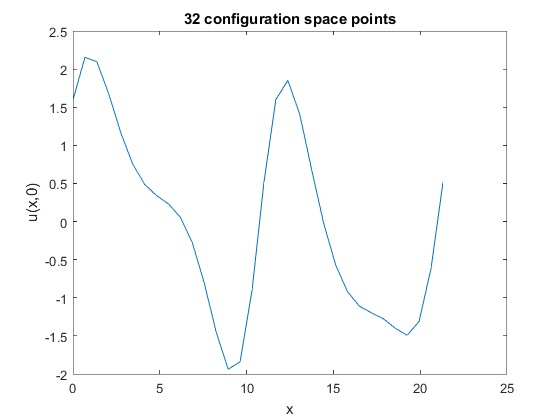
\includegraphics[width=\textwidth,height=.20\textheight]{MNGspec0}
  \end{minipage}
  \begin{minipage}[height=.20\textheight]{.48\textwidth}
    \centering \small{\texttt{(b)}}
    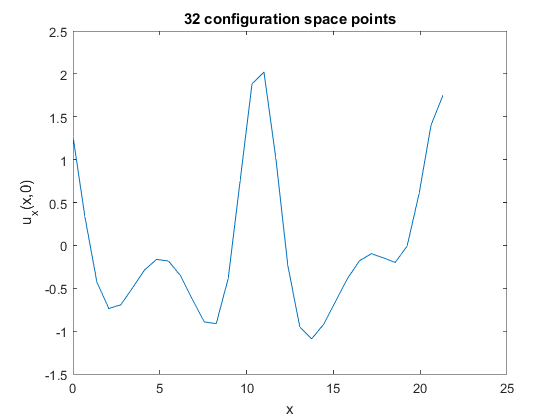
\includegraphics[width=\textwidth,height=.20\textheight]{MNGspec1}
  \end{minipage}
  \\
  \begin{minipage}[height=.20\textheight]{.48\textwidth}
    \centering \small{\texttt{(c)}}
    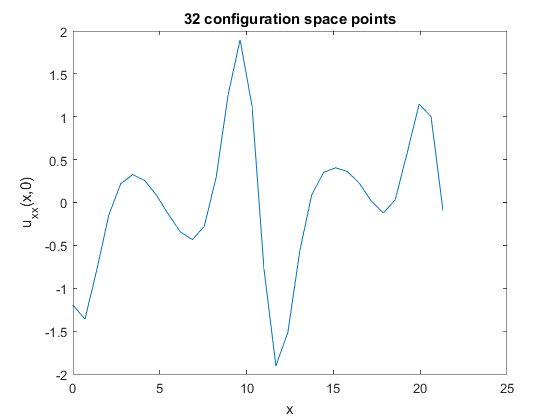
\includegraphics[width=\textwidth,height=.20\textheight]{MNGspec2}
  \end{minipage}
  \centering
  \begin{minipage}[height=.20\textheight]{.48\textwidth}
    \centering \small{\texttt{(d)}}
    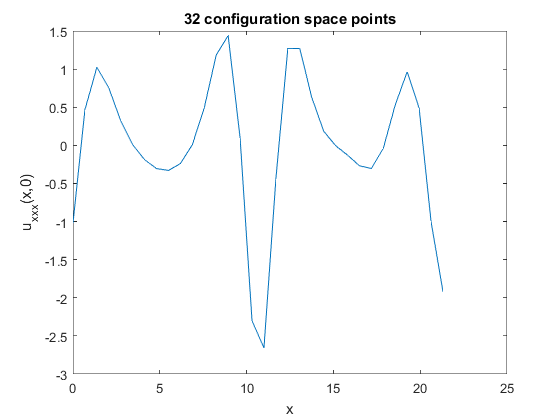
\includegraphics[width=\textwidth,height=.20\textheight]{MNGspec3}
  \end{minipage}
   \caption{ Results from Spectral Differentiation method \refeq{e-Spectralderiv} and comparison to $u(x,t)$.
   (a) $u(x,t)$, (b) $u_x(x,t)$,
   (c) $u_{xx}(x,t)$, and (d) $u_{xxx}(x,t)$.
            }
  \label{fig:MNGspecderiv}
\end{figure}

\MNGpost{2016-07-26}{

\begin{description}
\item[ErrorHunting]
Started looking at parts of the code that I may have been taking for granted. I thought most of the problems were arising from normalization issues, error tolerances, frequencies, spectral methods, and the actual integrator, \texttt{ode15s}, so that's where most of my time has been spent. Having still not achieved spatial integration for $x \in [0,22]$, I've been picking through everything for a while now to see if there's something I might have been taking for granted or overlooked.

Previously, I had checked the results from the time integrator by reproducing \reffig{fig:ppo1rpo1} in \reffig{fig:MNGtimeintL22}. Also, as an secondary check of periodicity, I plotted orbits in $u(x,t)$, $u_x(x,t)$, $u_{xx}(x,t)$ coordinates, and other combinations such as $u_x(x,t)$, $u_{xx}(x,t)$, $u_{xxx}(x,t)$ just to see if the time-integrated data formed a closed orbit, which they appeared to.

This being said, it seems I was unaware that checking the periodicity of derivatives calculated by spectral differentiation in \refeq{e-Spectralderiv} was insufficient. The derivatives don't seem to demonstrate the actual rates of change of $u(x,t)$, which might be why the spatial integration could be blowing up. As one can see in \reffig{fig:MNGspecderiv}. (Apologies for the custom paint job on the figures, I realized that the titles were incorrect after leaving the office.)

I found in \HREF{http://math.mit.edu/~stevenj/fft-deriv.pdf}{fftderiv} that one needs to treat the even and odd numbers of derivatives differently in terms of the form the wave numbers need to take, c.f. \textbf{Algorithm 1} \textbf{Algorithm 2}. When applying this to my code it didn't change the results from the spectral differentiation.

\MNGedit{Burak pointed out I was making a mistake. Updated the figures in response.
}

\item[RegardingPCpost] (I will also put these comments in the appropriate place in regards to the correspondence of the previous couple days.) \\
    The rapid oscillation of \reffig{fig:MNGFinit520} seems to only occur for the FFT corresponding to the $1st$, and $16th$ configuration space points when a resolution of $32$ points is used.

\end{description}
}
\MNGpost{2016-08-08}{
Was Ill for the majority of last week so I didn't accomplish much outside of my report, hence the lack of blog posts.

\begin{description}
\item[Dealiasing]
Instead of the so called "$3/2$ rule" delaliasing method (where the nonlinear term is
computed on a larger grid created by zero-padding arrays), I applied the so-called
"$2/3$ rule" where the values of the highest $1/3$ of Fourier coefficients are set to zero
when calculating the nonlinear term of \refeq{e-FksX}. Got the idea from \HREF{arXiv:math/0701337}{arXiv}.
This did not seem to help in any way after testing.
\item[Equilibrium test]
Tested spatial integration for initial condition that was constant in time (i.e. only nonzero
Fourier coefficient was the $0th$ mode. I wasn't completely sure what to do for the initial conditions
of the spatial derivatives so I assumed they fell under the same condition. I tested with multiple sets initial values for
the derivatives (the zeroth modes $\Fu^{i}_0 \quad i=1,2,3$). When all of the derivatives were set to zero,
there was no change in $u(\conf,\zeit)$ (done as a sanity check). When the initial conditions for the spatial derivatives
were taken from the time integration the values of $u(\conf,\zeit)$ (constant in time but not space) oscillate between negative and positive values
before escaping to $-\infty$. The amplitude of the Fourier coefficient $\Fu^{0}_0$ was the only nonconstant value.
\item[FutureWork]
I'm unsure where I should proceed from here. I am still searching for further improvements to my code but I am really running out of ideas,
other than scrapping the integration routine I am running and \emph{trying} to apply the ETDRK4 schema from \refref{ks05com}; which I'm not sure can
even be applied.
\item[MeetingRocklin]
Made plans to talk to Prof. Rocklin this Wednesday.
\end{description}
}

\MNGpost{2016-08-10}{
\begin{description}
\item[MeetingWithZeb]

I met with Professor Rocklin as was planned. We discussed topological transformable materials
and their implications and properties. The primary topic of this discussion was \textit{floppy modes}.
Which are soft deformations of the system with small energy costs. This is done in order to create materials
whose mechanical properties can change by means of such a transformation. We touched on other topics as well
such as elasticity theory and amorphous materials. Papers read/skimmed:
\HREF{http://arxiv.org/pdf/1510.06389.pdf}{arXiv:1512.06839v1 [cond-mat.soft]},
\HREF{http://arxiv.org/pdf/1510.06389.pdf}{arXiv:1510.04970v1 [cond.mat.mes-hall]},
\HREF{http://arxiv.org/pdf/1403.0936.pdf}{arXiv:1403.0936v1 [cond-mat.soft]}.

\item[KSspaceint]
I've been looking for more ways to change my code/find methods that are of use in spatial integration, looking for
different ideas across the internet and in \refref{trefethenSpectral}.

Tested whether or not the higher modes are corrupting the lower modes by doing different tests; namely forcing
higher modes to be equal to zero. This had no effect on the evolution of the lower modes who are so dominant the
behavior of $u(\conf,\zeit)$ was also unchanged.

Did more testing on the $2/3-rule$ dealiasing scheme. This showed marginal improvements over no aliasing, but it is better than
the $3/2-rule$ because it's cheaper computationally.
\end{description}

}

\MNGpost{2016-08-11}{

\begin{description}

\item[KSspaceint]
Looked at the spatial evolution of $u(\conf, \zeit)$ in a new way today in hope to get some new idea on how to make some progress.
I made the integrator plot $u(\conf, \zeit) = N \mathcal{F}^{-1} \left( \Fu^{0}_k \right)$ at every step and watched it like an animation.
What I observed was that $u(\conf,\zeit)$ is seemingly unchanged until
some critical point where the field seems to destabilize, at which point
the field inverts itself, and then at (usually one or two) a few points
diverges towards infinity. I investigated this further by introducing some
parameters into equation \refeq{e-FksX}. The most notable result from
this experimentation was that the equations became more stable after
making the contribution of $\Fu^{2}_k$ larger in comparison to the other
terms in,
\beq \nonumber
 \frac{\partial}{\partial \conf} \Fu^{(3)}_\ell =
        - i \omega_\ell \Fu^{(0)}_\ell
        \, - \Fu^{(2)}_\ell
        \, - \sum_{\ell' = -\infty}^{\infty} \Fu^{(0)}_{\ell - \ell'} \Fu^{(1)}_{\ell'},
\eeq
which I was not expecting due to how the terms behave in time integration.
\item[Windowing]
Looked into applying a windowing function in order to deal with spectral leakage and any discontinuities present; had little effect on the integration process but completely corrupted $u(\conf,\zeit)$. At least I learned something I suppose.

\item[ErrorCorrection]
I realized through my animation method described above that the
integrator was mishandling the initial conditions which caused a couple
of figures to display backwards time-behavior over spatial integration,
e.g. \reffig{fig:MNGcompxint}. I have uploaded new figures which should
be correct.
\end{description}
}

    \PCpost{2016-08-15}{
I do not quite understand ``until some critical point'' (you mean a value
of the integration coordinate $x$?) and ``at (usually one or two) a few
points diverges towards infinity'' (you mean values of time $\zeit$?)
while looking at $u(\conf, \zeit) = N \mathcal{F}^{-1} \left( \Fu^{0}_k
\right)$, but that might be a hint that there is something seriously wrong
with the concept of integration of these equations along the spatial
coordinate. But why then can one integrate it for the $\period{}=0$, \ie,
\eqva?

I have not yet put together
\refsect{sect:KStimeInt} and \refsect{sect:KSspaceInt}, and recast the
problem of finding a periodically repeating spatio-domain as a fixed
point condition, like Boris likes to do (allegedly - I have not seen the
formulas for the fixed point \jacobianM\ yet), but:

There are two ways of solving differential equations. One is as
integrate-forward problem, with given initial conditions - that is what
we are trying to do now.

The other is as a variational problem, where one makes a guess
loop\rf{CvitLanCrete02,lanVar1} (for a \po) or a guess torus\rf{LCC06}
(for an invariant torus, such as we search for here), and then defines an
error function that measures the integral squared of the local deviation
of the tangent space to the guess from the tangent space as defined by
the equations of motion at the point. That is guaranteed to converge by
{\descent}, for a decent enough initial guess (and our guess is the
numerically exact solution). The stability is $1-J$, and Boris says that
its determinant does not care whether one integrates time or space. Still not
obvious to me, but feels right.

What I am saying is that I still worry that your code has an error, such
that locally the tangent fields are not as given by the (instantaneous)
equations of motion. If there is any error in that, the integration must
go awry. Concretely, if tangents to surface your integrator sweeps out by
integrating the initial time-periodic state do not agree with the
tangents to the exact solution (the instantaneos equations of motion),
the code has an error. That is a \emph{local} test, it requires no
integration.
    }

\MNGpost{2016-08-16}{
\begin{description}
\item[Testing]
Did more code testing yesterday and today, but no progress to report.
\item[Report]
Small additions and edits to \texttt{reportMNG.tex}.
\item[Reading]
Began parsing through the literature on (variational) {\descent},
specifically \refrefs{CvitLanCrete02,lanVar1} and for invariant tori
\refref{LCC06}.
\item[MattToPC]
The derivatives at this stage are be calculated by spectral
differentiation method, if I'm understanding you correctly you're saying
if my tangent fields are wrong then the integration cannot proceed
correctly, which I agree with. Do we know of a way to check this outside
of something like finite difference methods?
    \\{\bf Predrag 2016-08-19}
Wish I knew. Whatever goes into the integration subroutine as the
equations to integrate must (instantaneously, or in one integration step)
satisfy \refeq{ks} and \refeq{e-MNGre11}.
\end{description}
}

\NBBpost{2016-08-18}{to Matt:

If I'm not mistaken, you have been trying to use Matlab's built-in integrators
most of the time. My suggestion for you is to look for implicit integrators
used for Hamiltonian systems, which are symmetric under time-reversal. We have
an analogous situation here since we have space-reversal symmetry. You can
start with the implicit midpoint method.}


    \PCpost{2016-08-18}{
I would not use much time on improving integrators at this stage (the
flow is not Hamiltonian, but there is lots of literature on time-reversal
invariant dynamical systems - \refref{lamb98,LaWu02,Bosetti2010} are a
few examples). We either have a bug in the code, or there is something
seriously amiss about the whole idea. First we need to go step by step
through the code, then someone re-derives the equations and writes an
independent code from the scratch. If two independent codes produce the
same trajectories, then we need to rethink the whole idea.
    }

\begin{figure}
\small{\texttt{(a)}}
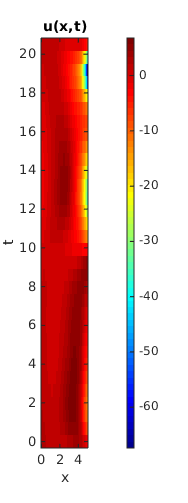
\includegraphics[width=0.2\textwidth]{MNGxintim5}
\small{\texttt{(b)}}
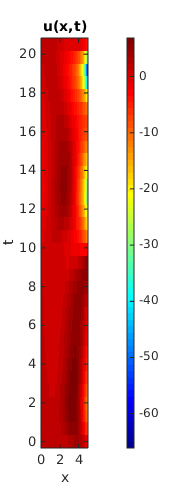
\includegraphics[width=0.2\textwidth]{MNGxintode15s5}
\small{\texttt{(c)}}
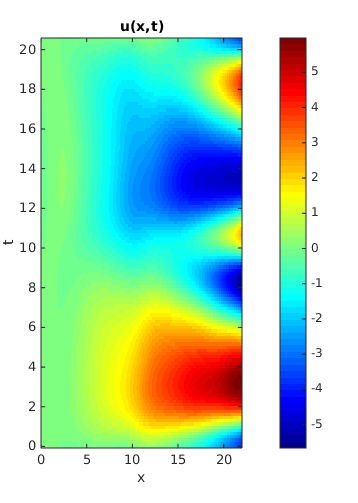
\includegraphics[width=0.37\textwidth]{MNGLIxint22}
\caption{\label{fig:MNGxintcomparison}
Spatial integration $x \in [0,5]$ comparison of integrators
(a) \texttt{ode15s} and
(b) implicit midpoint method. Initial condition was a time strip of
\PPO{10.2}.
(c) Spatial integration $x \in [0,22]$ using values for $u_{\conf \conf
\conf \conf}(\conf,\zeit)$ acquired from spectral differentiation as
opposed to evaluation of the \KSe. The implicit midpoint method was
employed as the integrator as I found it easier to control the step size.
}
\end{figure}

\MNGpost{2016-08-18}{:

\begin{description}
\item[MNGtoPC]
Would it be worthwhile to write up a step-by-step summary, i.e. a
walk-through, of my code and perhaps add it to my report?
    \\{\bf Predrag 2016-08-19}
Hope not - seems like too much work...
\item[ImplicitMidpointMethod]
According to \reffig{fig:MNGxintcomparison}\,(a) and (b)  my
implementation of the implicit midpoint method generates the same results
as ode15s, albeit at a slower pace. The figure includes spatial
integration data for $x \in [0,5]$ using the same initial condition as
usual, a time strip of \PPO{10.2}.
\item[AnotherTest]
I decided to test my integrator with one more (final?) method. Instead of
evaluating the Fourier coefficients $\Fu^{(3)}_k$ corresponding to
$u_{\conf \conf \conf \conf}(\conf,\zeit)$, during the integration
process using the \KSe, I generated them by
means of spectral differentiation using the initial condition.

I acknowledge that I am bypassing the entire point of my project but I
just figured I might as well test this case as I thought it might
demonstrate whether the accuracy of the derivatives I have been using all
along has been adequate. Sadly, not even this test will reproduce the
\PPO{10.2} orbit, as can be seen in \reffig{fig:MNGxintcomparison}\,(c).
I believe that this indeed shows that the inaccuracy is playing a larger
role than I might have initially anticipated, as even the values for the
derivatives taken directly from the time integration were inadequate in
reproducing the orbit. I used a spatial discretization of 1024
configuration space points in order to help smooth out the derivatives
for spatial integration, i.e. $x_n = n\,22/1024, \, n =0, 1, \ldots,
1024$.
\end{description}
        }

    \PCpost{2016-08-19}{
\refFig{fig:MNGxintcomparison}\,(a) and (b) are sure going off the charts:
\\
$u(\conf,\zeit) \to -65$. Flummoxed.
    }

\MNGpost{2016-08-20}{:
There are two different programs one can apply to regarding working at UC Santa Barbara.
\begin{description}
\item[Graduate Fellowship Program]
According to \HREF{https://www.kitp.ucsb.edu/apply/fellowships/graduate-fellowship-program}{Graduate Fellowship Program}
the process of the applying to the graduate fellowship program
is as follows:
the \emph{advisor} is required to fill
out a nomination form consisting of the
personal information of the student and
a short letter of recommendation for the program
and acknowledge the \textbf{minimum five month} stay at UC Santa Barbara.
(The student can also stay up to 6 months). They support up to
four graduate students at a time, either in Summer (July-December) or
Spring (January-June).

The student is reimbursed up to 2100 dollars a month for housing and
food; there is also a rather ambiguous statement about round-trip
travel "some assistance can also be provided".

The deadline for nominations for the January-June stay is September 1st,
while the deadline for the July-December stay is February 1st.

\item[KITP Affiliate Program]
I couldn't find a page describing this program other than the actual
form itself
\HREF{https://www.kitp.ucsb.edu/affiliate-nomination}{Affiliate Program Form};
wherein it requires the advisor's information/stay information,
information about the student or postdoc, and the
proposed stay for the student or postdoc. This is supposed to be a minimum of three
weeks.
If there is a plan for the student/postdoc to stay greater
than or equal to six weeks
financial support can be requested.

The main requirement is that the advisor has already
received an invitation;
I could not find deadline information
pertaining to this form; any questions are
supposed to be sent to the director of the
program via \HREF{https://www.kitp.ucsb.edu/contact/Director}{Contact Director}.
I sent a message via this link requesting the deadline information.
\end{description}
}

\MNGpost{2016-08-20}{:
With help of Lan and Cvitanovi{\'c}\rf{lanVar1} I rederived,
\[
\frac{\partial^2 \tilde{\conf}}{\partial s \partial \tau}
-\lambda A \frac{\partial \tilde{\conf}}{\partial \tau}
-v\frac{\partial \lambda}{\partial \tau} = \lambda v - \tilde{v}
\]
in order to get a better understanding of all of the working pieces
and where the terms originate from.

From what I understand, a guess loop (which is required to be a
relatively good guess to a periodic orbit) is parameterized/discretized
with variables $s_n$ (which has to be done carefully to avoid
clumping, which would destroy the numerical smoothness).
The periodic orbit is discretized with variable $t_n$.
Each point on this guess loop, L, has two important
vector quantities associated with it, namely, the loop tangent $\tilde{v}$
and the flow velocity $v$. A cost functional is minimized such that
after a process of continuous deformations parameterized by
fictitious time variable $\tau$
the two vectors converge in the limit of the loop $L$ approaches the
periodic orbit. The magnitudes of these two vectors are matched with
a scaling coefficient $\lambda = \frac{\Delta t_n}{\Delta s_n}$.

If I am understanding this correctly, in the scope of my problem, if a time
periodic orbit is taken to be the initial guess loop, then the flow velocities
take over the role of loop tangents, and the flow velocities role is replaced
with the corresponding spatial derivatives.

While I haven't begun the actual implementation of this I'm sure there are some
subtleties that I am missing out on, I especially have my doubts about whether
the form of variational equation should look the same as the role of time
is being replaced by a spatial variable, although perhaps I'm supposed to merely
view them as means by which the loop is parameterized.

The part that troubles me is that as far as I see this will not enable spatial
integration of infinite extent because the end result would be a spatially
periodic loop if functioning properly, but for my purposes this is
better than getting no results \ie, where my project currently stands
with direct spatial integration in Fourier space.
}

    \PCpost{2016-08-22}{
The \po\ examples\rf{CvitLanCrete02,lanVar1} illustrate the {\descent} idea. The power of the method is that arbitrarily long,
arbitrarily unstable long cycles can be found (see the long \KS\ orbit in
Fig.~6\,(d) of \refref{lanCvit07}; also $T=0$ spatial {\po}s of Sect.~III
could not have been found without the {\descent}). In our project we
are interested in determining a doubly-periodic time- and space-
translation invariant torus from a guess torus. An example, admittedly a
pretty mild one, is worked out in \refref{LCC06}.
    }

\MNGpost{2016-08-22}{:

\begin{description}
\item[MeetingWithPC]
Discussed the variational {\descent}
in the case of spacetime torus.
Briefly mentioned the motivation in regards to its benefits of stability
versus integration procedures. The main idea is that there are two
tangent spaces defined at each spacetime point. My goal is to
formulate fictitious time integration that minimizes a cost-functional
between these two tangent spaces.

This process will be implemented by minimizing the angle of separation between the tangent hyperplanes defined by the two tangent spaces. In order to have computational progression and not stall out, I must decide on a method of symmetry reduction in order to break both continuous symmetries present in the problem at hand: time and translational symmetries. By doing so I will force the system to evolve in a "tranverse" direction, i.e. the direction of interest.

\item[Variational Newton Method for spacetime torus]
We begin with an initial condition that takes
the form of a spacetime torus. In my case, this will specifically be the short
periodic orbit $\PPO{10.2}$ of the $L=22$ Kuramoto-Sivashinsky system.
The \statesp\ points \textbf{x} will be parameterized by
    \PC{2016-08-22}{that presupposes a very special parametrization, where
    all $s_i$ sit on unit circles. For example, the curvilinear length
    $ds = (\sum_i (dx_i)^2)^{1/2}$ is not normalized like that.}
$\mathbf{s} = ( s_1 , s_2, ... , s_m ) \in [ 0, 2\pi ]^m $ such that
\[
\mathbf{x}( \mathbf{s} +2\pi\mathbf{k} ) = \mathbf{x}( \mathbf{s} )
\quad \mbox{for all} \quad \mathbf{k} \in \mathcal{Z}^m.
\]

The torus we are searching for will be an invariant set of the mapping
\[
\mathbf{f}(\mathbf{x}(s)) = \mathbf{x}( \mathbf{s} + \mathbf{\omega}( \mathbf{s} ))
\]
where  \textbf{$\omega$} is the parametrization dependent shift.
With this initial condition, a fictitious time parameter $\tau$
is to be defined such that it parameterizes a continuous
transformation between the initial guess torus and the torus
invariant under the mapping (homotopy?).

The fictitious time evolution will be defined by the
minimization of a cost functional
    \PC{2016-08-22}{Have not wrapped my head around \refeq{MNGtorusCost} yet}
\beq
\mathbf{F}(\mathbf{s},\tau)^2 =
    \left(
    \mathbf{x}(\mathbf{s} + \mathbf{\omega}(\mathbf{s},\tau ), \tau)
    - \mathbf{f}(\mathbf{x} ( \mathbf{s},\tau))
    \right)^2
\ee{MNGtorusCost}

\end{description}
        }

\MNGpost{2016-08-23}{:
Still trying to understand the variational {\descent};

What I originally thought was that given the initial condition,
the time integrated solution \PPO{10.2}
(thanks for the ghostbusting)
defined on an $N \times M$ grid. $N$ is determined
by the spatial resolution/discretization and $M$
is determined by the number of time steps in
the integration process. For computational speed,
$N$ and $M$ should be taken to be powers of 2 to
exploit the speed of MATLAB's FFT algorithm.

For simplicity it's probably best to have $N=M$, but
for the sake of unambiguous subscripts I will keep it
as $M$ for the time being.
    \PC{2016-08-24}{please keep  $N$ and $M$ distinct. Ideally, use the
    same letters that Cats use in the \catlatt s project}
By doing so, the parameterization / discretization of the initial
condition becomes,
    \PC{2016-08-24}{please use a different letter for space length $s_1$}
\beq
\nonumber
\mathbf{s} = (s_1,s_2) = (x_n,t_m)
\eeq
where $x_n = \frac{n L}{N}$ and $t_m = \frac{m T}{M}$ for
$n = 0, \ldots, N-1$ and $m = 0, \ldots, M-1$.

With this discretization, I believe the tangent space defined over the
discretization and in terms of space and time Fourier modes becomes:
\beq
\mathbf{v}(\mathbf{s},\tau) =
    \begin{bmatrix}
    i \sum_{k} q_k a_k(\tau)e^{i q_k x_n} \\
    i \sum_{j} w_k b_k(\tau)e^{i w_k t_m}
    \end{bmatrix}
    \, \mbox{where,} \quad q_k = \frac{2\pi k}{L}, w_j =\frac{2\pi j}{T}
\ee{MNGTangentSpace}
with $k = -N/2+1, \ldots, N/2$ and $j= -M/2+1,\ldots,M/2$.

There are a number of things I am getting very confused with.
At first I thought I was going to be performing fictitious time
evolution such that a cost functional involving the tangent space
of the evolving torus and the tangent space of an invariant torus
would be minimized. In other words, I thought I would use the
definition for the tangent space in \refeq{MNGTangentSpace}
and evolve the torus until
\beq
\mathbf{v}(\mathbf{s},\tau)=
    \begin{bmatrix}
    \sum_{k} \dot{a}_k(\tau)e^{i q_k x_n} \\
    i \sum_{j} w_j b_j(\tau)e^{i w_j t_m}
    \end{bmatrix}
\ee{MNGTangentSpace2}
where $\dot{a}_k$ is calculated from the representation of \KSe\
used for the time integration of the spatial Fourier modes \refeq{e-Fksex}.
This is what I thought at first, but by doing so I will be neglecting
\refeq{e-FksX} in this process, although I don't see how to incorporate
\refeq{e-FksX} as this would introduce four independent variables for
the temporal Fourier modes, making my 2-torus into a 5-torus?
    }
    \PCpost{2016-08-24}{
It does not matter how many dimensions it is embedded in, and how many
first-order equations you have, the torus is 2\dmn, one dimension for
each continuous symmetry. It's tangent space is a 2\dmn\ plane embedded
in your $N \times M$ dimensions. You compute it by doing infinitesimal
shifts in time and space, \ie, by taking derivatives... I think.
    }

\MNGpost{2016-08-24}{
Also by keeping the second component constant I believe I'm ignoring parts
of the dynamics.
\MNG{2016-08-24}{I believe this is okay as the Fourier coefficients depend on the
fictitious time $\tau$ so it's not holding anything constant in actuality.}

One of the other reasons why I believe I don't understand what's going on is
because in Lan's paper\rf{LCC06}, his formulation of the cost functional
\refeq{MNGtorusCost} includes the difference between the mapping \textbf{f}
and the {\statesp} representation of the torus \textbf{x}. I'm quite
confused how to formulate the mapping in this circumstance, unless this is
exactly the point, meaning that it's numerically determined by the
fictitious time evolution of the \jacobianM.

In short, I still have a lot of work to do in order to understand this method.
}

\MNGpost{2016-08-24}{: Spent the day reading Schilder \etal\rf{SOHV05} and
rereading \refref{CvitLanCrete02}, Lan and Cvitanovi{\'c}\rf{lanVar1}, as well as \refref{LCC06} in hopes of
better understanding this method.

In regards to some of the statements in my blog post yesterday; for a torus
to be invariant after the application of \textbf{f}, which is the
criterion that we're using to guide the fictitious time evolution according
to \refref{LCC06}, the only intepretation my brain can think of is that
\textbf{f} represents the tangent space of the torus that results from
this fictitious time evolution. If so I feel like maybe I was a little
hasty in my judgment of the equation I came up with for the mapping
\textbf{f}, namely \refeq{MNGTangentSpace2}.

For a little more investigation of \refeq{MNGtorusCost}, I
believe the reason behind the $\omega$ in the term
$\mathbf{x}(\mathbf{s},\omega(\mathbf{s},\tau),\tau)$ is that
the orbit reached by fictitious time evolution \textit{could}
be a \rpo\ as opposed to a \ppo. In this case the application
of the \textbf{f} would not leave the orbit unchanged after one
period until the corresponding shift is taken into account?
That is of course if my interpretation of \textbf{f} is indeed
the flow field. The only other idea I've been able to think of is
some sort of circle map that permutes items around the discretization.

This is why I still don't understand why \textbf{x}
is in \refeq{MNGtorusCost} as opposed to \textbf{v}.

On how one can handle this quantity, $\omega$, it may or may not
be fixed a priori, and one can use the following rules: for a fixed
shift equal to $\omega$ one must require
\beq
0 = \frac{\partial\omega}{\partial\tau}
\eeq
while for searching for an torus of a "given topology", one must
employ what Lan refers to as the \textit{phase condition}
\beq
0 = \oint ds \,\mathbf{v} \cdot \frac{\partial\conf}{\partial\tau}
\label{e-MNGphaseCond}
\eeq
where \textbf{v} is a $[ d \times 2]$ dimensional tensor, where
$d$ is the dimension of the statespace. \textbf{x} incorporates both the spatial and temporal Fourier modes so
it is $[2\times d]$ in size.
}

    \PCpost{2016-08-24}{
Sorry, I have to go to bed now, and might not be able to help in days ahead.
For specific questions, ask

\noindent
Yueheng Lan
\\
Home:	yueheng\_lan@yahoo.com
\\
Work	lanyh@bupt.edu.cn
\\
Mobile	+86861013520900575
\\School of Science,
Beijing University of Posts and Telecommunications
\\
Skype	yueheng\_lan


    }

\MNGpost{2016-08-29}{
\begin{description}
\item[CodeFromLan]
Received some code from Lan, trying to interpret it at the moment;
I have no experience in Fortran so at best
I'm trying to get a sense of
what he has done so that I can start to produce my own code.
\item[Readings]
Still trying to figure out the best way to implement variational {\descent} code. Read Fox\rf{FoxCvi14} \textit{A brief life and death
of a torus, computation of quasiperiodic solutions to the
kuramoto-sivashinsky equation} and skimmed through a number of papers,
with the most time spent on Rasmussen and Dieci\rf{RasDie08}, and Ge and
Leung\rf{GeLe98}.
\end{description}
}

\PCpost{2016-08-30}{
Thanks for checking the literature! Remember, our torus is much easier
than what most literature tries to find - it suffices to find the \rpo\
in the time direction, with period $L$, the torus is then swept out by a
rigid rotation by $L$ in the spatial direction. Finding invariant tori
not due to symmetries (like
\refrefs{LCC06,paskauskas2008,paskauskas2009a,} and the above Fox
manuscript\rf{FoxCvi14}) is very interesting, but do not work too hard on that right
now - our spatiotemporal domain is ``trivial'' in the spatial direction.

Here, for completeness are some more torus papers:
\rf{HanBer80,CheSu90,toricgl,Leis97,GL-Tsa03,SOHV05,SaNeSi10,
FigHar12,SanNet13,LROBK13,FoxPhDthesis,Fox14,FoxMei16}. Just to glance
at, not necessarily read in any depth.
}

    \PCpost{2015-09-15}{
(reposted here from \texttt{elton/blog/AdamBlog.tex})

Reading about robustness of invariant tori. Farazmand likes to refer to
Fenichel\rf{Feniche71} (to read it,
\HREF{http://chaosbook.org/library/Feniche71.pdf}{click here}). My
understanding is that if a stability exponent is purely imaginary, it
can destroy a torus at an rational resonance; but if it has a real part
(hyperbolic case), there is no way for the Floquet exponent to approach
the purely imaginary winding number of the torus, there can be no
resonance, and the torus remains smooth and robust for an open interval
of the system parameter values.

Figueras and Haro\rf{FigHar12} write:
``it has been known for a long time that persistence of invariant
manifolds is closely related to the concept of normal
hyperbolicity\rf{Feniche71,Sacker65}. %21
%34 M. W. Hirsch, C. C. Pugh, and M. Shub, Invariant manifolds,
%    Lecture Notes in Math. 583, Springer-Verlag, Berlin, 1977.
%50 R. Ma\~{n}\'e, Persistent manifolds are normally hyperbolic,
%   Trans. Amer. Math. Soc., 246 (1978), pp. 261-283.
We consider the analogous
concept, tailored for skew products over rotations. Roughly speaking, an
invariant torus is fiberwise hyperbolic if the linearized dynamics on the
normal bundle is exponentially dichotomous, that is, the normal bundle
splits into stable and unstable bundles on which the dynamics is
uniformly contracting and expanding, respectively. Notice that the
tangent dynamics is dominated by the normal dynamics, since the former
presents zero Lyapunov exponents. This implies that fiberwise hyperbolic
invariant tori are robust and are as smooth as the system [ 28 ].
% A. Haro and R. de la Llave, A parameterization method for the
% computation of invariant tori and their whiskers in quasi-periodic maps:
% Rigorous results, J. Differential Equations, 228 (2006), pp. 530-579.
''

Figueras' thesis might be an easier read:
\HREF{http://www2.math.uu.se/~figueras/preprints/files/phd_thesis/Jordi_LLuis_Figueras_Romero_PHD.pdf}
{click here}.
    }

\MNGpost{2016-08-31}{
\begin{description}
\item[Bib]
Skimming Dieci, Lorenz and Russell\rf{DiLoRu91}, but
I get lost in the mathematical formalism.
\item[KSspaceInt]
Tried some new ideas but they didn't accomplish anything and weren't
very well founded anyway.
\item[TalkWithBoris]
Had a preliminary meeting with Boris talking about some of the spatial
integration results. He said he would think on whether the divergent
results are fundamental to the equations and if there is some method
to keep the spatial integration bounded without changing the nature
of the equations. We scheduled a meeting at 3 pm Thursday
September 1st.

\item[Reason behind my confusion:]
I think the reason why I've been so confused for the past
week or so is due to Lan\rf{LCC06} and Fox\rf{FoxCvi14},
i.e. I was mixing up two different methods.

\textbf{I'm going to include what I had already typed up for completeness,
but I want to reiterate that I was mistaken on what I needed to do.}

\begin{itemize}
\item Fox\rf{FoxCvi14} evolution process for a 2-torus involves the use
of \PoincSec s to reduce it to a mapping of a 1-torus. The
section is taken, due to its simplicity, is normally a hyperplane of
codimension 1. This also reduces one of the two continuous symmetries
inherent in the problem, \ie, invariance under time translations.
\item The remaining \SOn{2} continuous symmetry can be handled by an
additional condition, for instance the ``phase condition" in
\refeq{e-MNGphaseCond}, which ensures that the ``average motion of points
in the loop equals zero"\rf{LCC06}.
\item The initial condition is then taken to be a loop on the \PoincSec; How one decides on the points taken is still unknown to me. I
thought they might be generated by just evolving the system in time or space
via the equations \refeq{e-FksX} and \refeq{e-Fksex} but I'm not sure.
\item Together with the initial condition and the {\descent} equation,
\beq
\frac{\partial \conf}{\partial \tau}(s + \omega, \tau) + \frac{\partial \conf}{\partial s}(s + \omega, \tau)\frac{\partial \omega}{\partial \tau}(\tau) - J(\conf(s,\tau))\frac{\partial \conf}{\partial \tau}(s,\tau) =
f(\conf (s,\tau))-x(s+\omega,\tau),
\ee{MNGNewtonDescent}
one performs fictitious time integration until the maximum of the cost
functional \refeq{MNGtorusCost}, evaluated over the loop points is less than a
certain cut-off threshold. \item The previous part takes a nontrivial inversion
of the \jacobianM\ due to it being so large. This was done with a combination
of LU decomposition and using the LU-Decomposition to approximate the inverse
\end{itemize}
\textbf{Work In Progress/Comments}
\begin{itemize}
\item Trying to understand why the \jacobianM\ in \refref{LCC06} only has one
index, as it is supposed to represent a matrix. Also puzzling to me is how
it can be represented as a single Fourier series.
\item I'm working on trying to figure out if the \PoincSec\
formulation will really work for me.
\item In a discussion with PC I was told to work with the tangent
space in a manner that would involve two different systems of autonomous
ODEs. Namely, the spatial evolution equations of \refeq{e-FksX} and the
time evolution equations \refeq{e-Fksex}. I'm unsure if it was meant to just
use one of these systems for evolution and then look at the tangent spaces or
to use both in some combined manner. I imagine I would use one as the spatial
and temporal Fourier modes both depend on $u(\conf,\zeit)$ but I'm not sure
if this would just reproduce previous results or would take things a step
further.
    \item
Fox\rf{FoxCvi14} mentions that the the function \textbf{f} in
\refeq{MNGtorusCost} is actually the Poincar{\'e} return map, so I'm
trying to figure out how one can the deduce the derivatives needed in
order to compute the \jacobianM.
\end{itemize}


\end{description}
}

\MNGpost{2016-09-01}{:
The following is a description of the meeting with Boris
and Predrag.

Boris said he hadn't yet looked at my blog for results,
but his main concern is whether the problems I have are
fundamental or numerical, as are seemingly everyone's
feelings about my project.

One of Boris' main suggestions were to check the spatial integration
for the zeroth mode, and see what the results are.

Another suggestion was to examine the stability of the
$u(\conf,\zeit)=0$.

There was much discussion on \refeq{BGsecret1} and whether or not there
is actually a constant term present that was not previously accounted
for. For the specific cat map example it seems that this constant is not
present, which is why it had previously eluded Boris. (I think?)

The idea was brought up that somehow the spatial direction reflection
symmetry (analogue of time reversal for time direction) was affecting the
spatial integration in a manner that has so far been unaccounted for.
Also was the idea that somehow the stability in the time-direction would
cause instability in the spatial direction; leading to the idea of
perhaps taking a smaller temporal domain as the initial condition, much
like how one would take a smaller spatial domain in the time-integration
process in order to provide stability. Noted in this discussion were the
$T=0$ domain from Lan\etal\rf{lanCvit07,DoLa14} solutions, and the
sequence of bifurcations that occur (in time direction) as domain size
$L$ is increased.
}

\MNGpost{2016-09-02}{
{\bf Spatial integration of the zeroth Fourier mode}
Adapted the code for spatial integration of the zeroth
temporal Fourier mode. Because this is a purely real quantity,
one can plot the amplitude versus spatial variable \conf,
as can be seen in \reffig{fig:MNGzmxint11}.
The integration blows up ($\Fu^{(0)}_0 \rightarrow -\infty$)
at $\conf \approx 12.292453$, so in order to capture what
happens before this divergence the plot represents the value
of the zeroth Fourier coefficient for $\conf \in [0,11]$.
    }

%    \PC{2016-09-08}{Where is figure fig:MNGxintZeroM?}
%    \MNGedit{2016-09-09}{That's just what I first called \reffig{fig:MNGzmxint11},
%        removing it somehow eluded me.}
%%%%%%%%%%%%%%%%%%%%%%%%%%%%%%%%%%%%%%%%%%%%%%%%%%%%%%%%%%%%%%%%%%%%%%
\begin{figure}
\centering
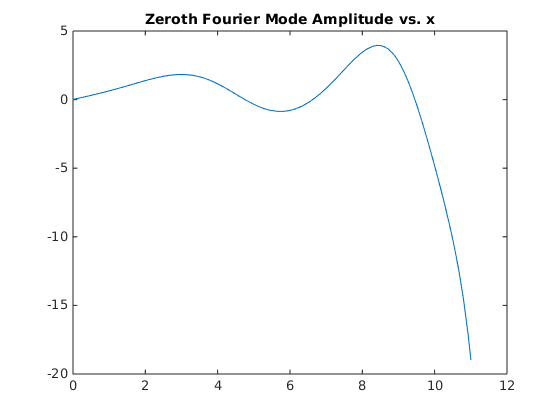
\includegraphics[width=.45\textwidth]{MNGzmxint11}
\caption{\label{fig:MNGzmxint11}
Value of the zeroth Fourier coefficient versus the spatial
variable $\conf$ for spatial integration $\conf \in [0,11]$.
The initial time-periodic loop was retrieved from time integration of
\KSe\ using \texttt{ksint.m} over $T = [0, 2\,T_{\PPO{10.2}}]$
using 1024 steps.}
\end{figure}
%%%%%%%%%%%%%%%%%%%%%%%%%%%%%%%%%%%%%%%%%%%%%%%%%%%%%%%%%%%%%%%%%%%%%%

\PCpost{2016-09-02}{
To me your initial version of the spatial {\stabmat} \refeq{MNGeqvaStblty} looked too diagonal -
it is all off-diagonal, I tried to rewrite it in \refeq{PCeqvaStblty}
(also, more logically, in the increasing order of $\Fu{}^{(J)}$).
\PCedit{(has been fixed since I wrote the above comment)}.
However, Boris has a quick way to the eigenvalues in terms of a quartic
equation, he'll show you how. Basically, in spatial evolution we seem to
have a repeller, not a strange attractor, and all spatial evolution will
take off to infinity, unless we ensure it is staying on the repelling
set. We kind of know that already from the $T=0$ spatial evolution.
    }

\MNGpost{2016-09-02}{
{\bf Stability of u=0 \eqva}
By rearranging the system of ODEs of \refeq{e-FksX}, the velocity gradients
matrix  $\Mvar$ evaluated with $u=0$ takes the form,
\beq
\Mvar(\mathbf{0}) =
\begin{bmatrix}
  0 & 1 & 0 & 0 \\
  0 & 0 & 1 & 0 \\
  0 & 0 & 0 & 1 \\
  Diag\{-i \omega_k\} & 0 & -1 & 0
\end{bmatrix}
\ee{MNGeqvaStblty}
\MNG{2016-09-05}{\MNGedit{Sleep deprivation : I had originally written
this in the wrong order because it looked pretty}}
where each entry is of size $N \times N$ where $N$ is the number of temporal
Fourier modes kept in the truncation. (i.e. $1 = I_N$) and
$\omega_k = \frac{2 \pi k }{T}$ for $k = -N/2+1, \ldots, N/2$.

The eigenvalues (stability exponents $\eigExp[j]=\eigRe[j]+i\eigIm[j]$)
of this {\stabmat} for a system of 32 Fourier modes (i.e. the size of
$\mathbf{A} = [128 \times 128]$) can be categorized in the following
manner:
\begin{itemize}
\item
60 stability exponents with positive real parts, $\eigRe[j]> 0$, with the
largest being the complex conjugate pair
$\eigExp[\pm] \approx 1.1985 \pm i 0.6154$
\item
60 stability exponents with negative real parts, $\eigRe[j]<0$,
\item
2 stability exponents equal to zero (up to machine precision).
\item
2 purely imaginary stability exponents, $\eigExp[j]=0 \pm i$
\end{itemize}
    }

\PCpost{2016-09-08}{
This numerical spectrum looks like what Boris would expect from his quick
way to get the eigenvalues in terms of a quartic equation, I guess you
two have not talked about it yet. You do not mention it, but the negative
exponents are the reflections of the positive ones, you might want to
arrange $j$ range in such a way that $\eigRe[-j]= - \eigRe[j]$. You
should get exact analytic formula for this spectrum as a solution of a
quartic equation.

The easiest way to survey the spectrum is to plot it
the $(\eigRe,\eigIm)$ plane; as an example I take a random stability
exponents plot from my \pCf\ work with Gibson and Halcrow,
\reffig{fig:newfp-lambdaplot}. That flow is dissipative (no
``time''-reversal invariance), so you expect a few expanding (positive)
exponents, few marginal due to symmetries, and infinity of negative ones.
In the case at hand, spectrum is symmetric under $\eigRe[-j]= - \eigRe[j]$,
so it will suffice to plot the $\eigRe[j] \geq 0$ half-plane.

By the way, do not plot multipliers $\ExpaEig_j$ for \eqv\ solutions
in the complex plane like Marcotte and Grigoriev do. That is nonsensical
for \eqva; to get a multiplier, you have to pick a (totally arbitrary
and unnatural) $T$ in the formula  $|\ExpaEig_j|=\exp(T\eigRe[j])$.
    }

%%%%%%%%%%%%%%%%%%%%%%%%%%%%%%%%%%%%%%%%%%%%%%%%%%%%%%%%%%%%%%%%%%%%%%
\begin{figure}
\centering
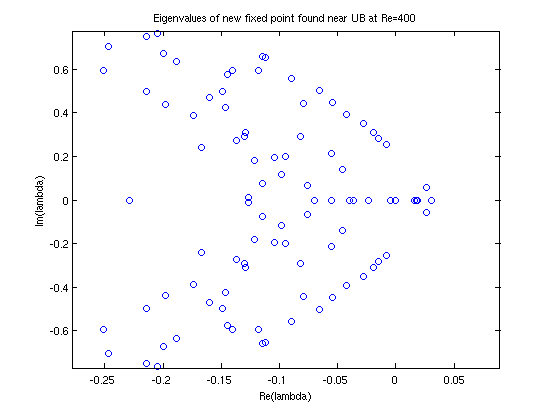
\includegraphics[width=.75\textwidth]{newfp-lambdaplot-zoom1}
\caption{\label{fig:newfp-lambdaplot}
Stability eigenvalues spectrum for one of the \pCf\ \eqva\ studied by
Halcrow, Gibson and Cvitanovi\'c (unpublished). Just an example of the
spectrum, not the one we are studying here.}
\end{figure}
%%%%%%%%%%%%%%%%%%%%%%%%%%%%%%%%%%%%%%%%%%%%%%%%%%%%%%%%%%%%%%%%%%%%%%



\MNGpost{2016-09-02}{
Predrag stopped in to see how I was doing and asked me to also determine
the eigenvalues of the {\stabmat} for the zero-mode only system i.e. the
eigenvalues of the $[4\!\times\!4]$ {\stabmat}, in order to verify whether the
spatial integration results of \reffig{fig:MNGzmxint11} are valid. My
question, is where the {\stabmat} should be evaluated, presumably near the
point of divergence? i.e. ($\conf \approx 12.292453$)?
}

\PCpost{2016-09-08}{
$u(x,t)=0$ is an \eqv\ both in the temporal and spatial direction. So I
would first look at stability eigenvalues (stability exponents) of the
spatial stability matrix on the $T=0$ temporal ``strip'', along the $x$
axis. That is, first the zero with temporal strip, than a small $T$ temporal
strip. Not sure about this...
    }

\PCpost{2016-09-02}{
I guess I do not know what \reffig{fig:MNGzmxint11} means. I meant that
if you start with $T=0$ spatially periodic profile (but not changing in
the time direction) its evolution is given by 4 ODEs, uncoupled to
evolution for any other initial time. So you need it to initialize the
four $u^{(I)}(0,\zeit)$ with precise values corresponding to one of our
\eqv\ or \reqv\ points, the same four numbers for {\em every $\zeit$}.
For that you need to use one of our \eqv\ or \reqv\ solutions, not the
\rpo\ \PPO{10.2}. After Fourier transform one still has 4 precise numbers
$\Fu^{(I)}_{0}$, and the rest of Fourier components vanishes.
    }

% \MNGpost(2016-09-02){ Made a small edit, read PC posts.}

\MNGpost{2016-09-06}{ {\bf KsSpaceInt}
Performed spatial integration on a time-strip from one of the equilibrium solutions
of \KSe\ , received from
Xiong's data file \texttt{ksReqx32.h5}. I believe that this corresponds to
$\EQV{1}$ of \refref{SCD07}, due to the label in the data file. I can't seem to locate
my flash drive that had the plot on it, but the general procedure was familiar.
I took a time-strip of values (now constant) and attempted spatial integration.

The resulting behavior was a monotonic decrease of the zeroth mode
Fourier amplitude to negative infinity, seen in \reffig{fig:MNGeqvaint8}
differing from the result of \reffig{fig:MNGzmxint11},
where I integrated the zeroth Fourier mode data retrieved from a time strip of \PPO{10.2};
I think this is worth mentioning because it seems that by using an equilibrium as the
initial condition for spatial integration behaves much worse, however this
could be idiosyncratic property of the particular time strip used.
    }

\PCpost{2016-09-10}{
To me
\reffig{fig:MNGeqvaint8} and \reffig{fig:MNGzmxint11} look comparable.
Can you replot \reffig{fig:MNGeqvaint8} as $\log|u(x,0)|$? I expect that would give you
a straight line, whose slope is the leading spatial stability exponent.
    }

\MNGpost{2016-09-06}{
\begin{description}
\item[TalkWithPC]
Discussed the apparent truth that we are dealing with a strange repeller.
As I grasp it, this is not necessarily confirmation that my code is
performing its duties, there could still be some numerical issues, but
the repeller guarantees that these are the death of any attempt to
reproduce \PPO{10.2}. The best way to handle this problem seems to be the
variational {\descent}. I currently have Fortran95 code sent to me by
Lan that produces invariant tori, but I'm new to Fortran and don't quite
understand it. \textbf{PC} mentioned I should talk to Lan and ask him
about code that produces periodic orbits as opposed to tori for the time
being, and to learn Fortran via by my own merits (and perhaps Xiong's).

\item[NewtonDescent]
Sent an e-mail to Lan asking for direction towards the codes for finding periodic orbits
using Newton method.
\end{description}
}

\begin{figure}
\centering
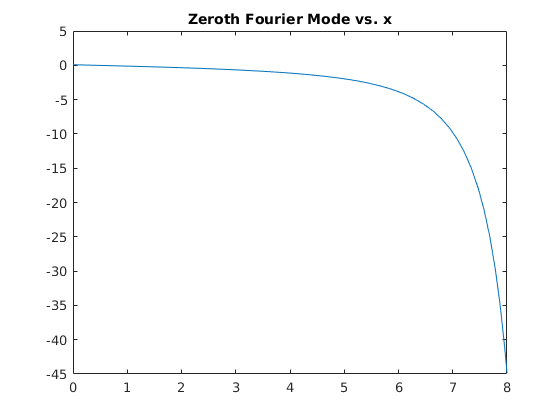
\includegraphics[width=.45\textwidth]{MNGeqvazmint8}
\caption{\label{fig:MNGeqvaint8}
Plot of the amplitude of the zeroth temporal Fourier mode coefficient
versus $\conf$ for $\conf \in [0,8]$. The initial condition is a time strip of
(identical) values taken from the first equilibrium $\EQV{1}$, in the notation
of \refref{SCD07}.}
\end{figure}

\MNGpost{2016-09-07}{
%\begin{description}
%\item[KSspaceInt]
%Here's the figure that I couldn't include yesterday
%This displays the monotonic divergence towards $-\infty$ that I claimed yesterday.
{\bf Fortran}
Spent most of the day so far learning how to code in Fortran, trying to walk
through some of Lan's codes. I feel like I learned quite a bit; I also ended
up finding his Fourier transform code online, as it was taken from
\textit{Numerical Recipes}.

I wonder if it would be worthwhile to re-do my spatial integration code
in a different language and
see if the results are identical. I feel like this wouldn't be too taxing with enough help
from \textit{Numerical Recipes}\rf{Press96}.
    }


%\PCpost{2016-09-08}{FIXED NOW
%Somebody has entered a non-ASCII character into an entry in \emph{siminos.bib},
%cannot figure out which one. That's why the compilation now always gives 2 errors;
%the first one is due to my laziness in including {\em appendStatM.tex}, but
%the second is a typo somewhere in the bib file...
%    }

\begin{figure}[h]
\begin{minipage}[height=.25\textheight]{.32\textwidth}
\centering
\small{\texttt{(a)}}
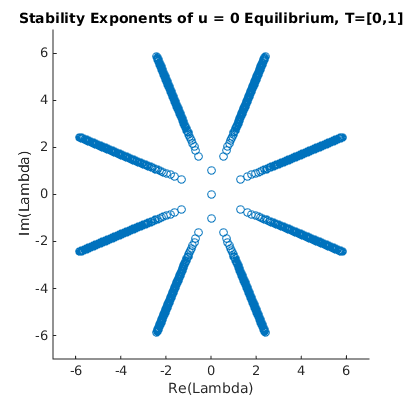
\includegraphics[width=\textwidth]{MNGstbexp1}
\end{minipage}
\begin{minipage}[height=.25\textheight]{.32\textwidth}
\centering
\small{\texttt{(b)}}
\includegraphics[width=\textwidth]{MNGstbexp100}
\end{minipage}
\begin{minipage}[height=.25\textheight]{.32\textwidth}
\centering
\small{\texttt{(c)}}
\includegraphics[width=\textwidth]{MNGstbexp10000}
\end{minipage}
\caption{\label{fig:MNGeqvastbexp}
$(\eigRe[j],\eigIm[j])$ complex plane plots of the stability exponents
$\eigExp[j]=\eigRe[j]+i\eigIm[j]$ for the
stability matrix from
\refeq{MNGeqvaStblty},
 512 Fourier modes were kept in each instance, meaning
the stability matrix is of size $2048 \times 2048$. The
temporal extent for each plot is
(a) $T = [0,1]$, (b) $T = [0,10]$, and (c) $T = [0,10000]$
}
\end{figure}


\MNGpost{2016-09-09}{:
\begin{description}
\item[Yesterday]
I was learning Python, gave up on Fortran due to suggestions.
I think I should be able to program a variational {\descent} code with a little
bit more Python practice.

\item[Stability exponents]
I'm including three separate plots \reffig{fig:MNGeqvastbexp}
of the stability exponents $\eigExp[j]$ for the
$u(\conf,\zeit) = 0$. Equilibrium of a temporal strip of differing \period{},
 but with the
number of modes constant. The only effect that the differing
temporal extents have on \refeq{MNGeqvaStblty} is on $w_k = {2 \pi k}/{T}$.
In all three figures I've kept
$512$ temporal Fourier modes, meaning that the stability matrix
is of size: $2048 \times 2048$.

The temporal extents of each, $T = [0,1]$, $T = [0,100]$, $T = [0,10000]$,
were chosen because they elucidate
different patterns when plotted on the complex plane;
however, I'm not sure if this is meaningful
because, again, the different temporal extents only affects
the frequencies $w_k$. Also, $10000$ seemed absurdly
large but I was curious to what happened at an extreme
range.
\end{description}
}

\PCpost{2016-09-10}{
Mhmmm - not sure what to make of $\eigIm[j]$ in the $(\eigRe,\eigIm)$
plane plots of \reffig{fig:MNGeqvastbexp}. Anyway, Boris says assume that
eigenvector of the $u(x,t)=0$ \eqv\ is of form $\sin(\omega t)\exp(k x)$
(missing some $2\pi$'s and $T$'s), stick it into the \KSe, you get a
quartic equation for $\eigExp[j]$. The eigenvalues plotted in
\reffig{fig:MNGeqvastbexp}, their symmetries and their multiplicities
presumably follow.
    }

\PCpost{2016-09-12}{ to Matt:
Does \refeq{e-FksSpattemp} explain your \reffig{fig:MNGeqvastbexp}?
Happy birthday!
    }

\MNGpost{2016-09-12}{
There was a missing factor of $-i$ in the $\omega_\ell$ term in
\refeq{e-FksSpattemp}. It comes from to the time derivative of the
Fourier expression for $\Fu_{k,\ell}$. I corrected \refeq{e-FksSpattemp}.
I wasn't getting equivalent scatter plots for the solutions to the
(initial, erroneous) quartic equation \refeq{e-FksSpattemp} and the
stability exponents of \refeq{MNGeqvaStblty}, which lead me to find the
error.
}

\begin{figure}[ht]
  \begin{minipage}[height=.32\textheight]{.45\textwidth}
    \centering \small{\texttt{(a)}}
    \includegraphics[width=\textwidth]{MNGstbexp8}
  \end{minipage}
  \begin{minipage}[height=.32\textheight]{.45\textwidth}
    \centering \small{\texttt{(b)}}
    \includegraphics[width=\textwidth]{MNGquareq8}
  \end{minipage}
   \caption{\label{fig:MNGstbspec8}
   Plots of (a) the spatial stability exponents of \refeq{MNGeqvaStblty}, (b)
   solutions to the (corrected) quartic equation \refeq{e-FksSpattemp}. 8
   temporal Fourier modes.}
\end{figure}
\MNG{2016-09-22}{Copied the wrong plot to flash drive, will update MNGquareq8 tomorrow}
\begin{figure}[ht]
  \begin{minipage}[height=.45\textheight]{.45\textwidth}
    \centering \small{\texttt{(a)}}
    \includegraphics[width=\textwidth,height=.45\textheight]{MNGeq1time}
  \end{minipage}
  \begin{minipage}[height=.45\textheight]{.45\textwidth}
    \centering \small{\texttt{(b)}}
    \includegraphics[width=\textwidth,height=.45\textheight]{MNGeq1space}
  \end{minipage}
   \caption{Integration of $\EQV{1}$ from \refref{SCD07}, periodic
   on domain $L=22$, (a) in time, using \refeq{e-Fks},
   and (b) in space, using \refeq{e-MNGmodifiedFksX}.
   The initial condition for the spatial integration was the time strip
   $u(\conf,\zeit)$, $\conf = L/2$, $\zeit = [0,T)$, where
   T happened to be $2\,\PPO{10.2}$, for no particular reason.
   Also, in order to produce the spatial integration plot, a spatial
   shift equal to $\frac{68 L}{128}$ was employed.}
  \label{fig:MNGeqva1spttmp}
\end{figure}

\begin{figure}[ht]
\centering
\includegraphics[width=.5\textwidth]{MNGeqva1error}
\caption{\label{fig:MNGeqva1error}
    Absolute error between time integrated and spatially integrated
    solutions of $Eq_1$.
}
\end{figure}


\MNGpost{2016-09-12}{: Thank you for the birthday wishes.
It's actually really timely because I have quite good news today.

\begin{description}
\item[EqvaStbExp]

Even with the corrected \refeq{e-FksSpattemp}, the spectra of
\reffig{fig:MNGstbspec8} only agree up to an exchange of the real and
imaginary parts. I haven't quite figured out why this is, but during my
experimentations I found that modifying \refeq{MNGeqvaStblty} in certain
ways produces exciting results.

\item[ModifiedFksX]
If I introduce a sign change to the identity matrices on the
super-diagonal of \refeq{MNGeqvaStblty}, the two formulas for eigenvalues
agree.
    \PC{2016-09-13}{you do not mean ``approximately agree,'' you mean
    ``exactly,'' \ie, to the numerical accuracy of whatever program you
    are using to compute the eigenvalues, right?}
Likewise if I changed the sign of the diffusion term in the bottom row of
\refeq{MNGeqvaStblty}, the spectra agree.

The really interesting part comes when you apply both of these
transformations; it leaves the stability exponent spectrum invariant,
leaving me to believe I had stumbled upon some sort of symmetry. The
corresponding modified equations \refeq{e-MNGmodifiedFksX} after such a
transformation are as follows (only sign changes),
\bea
\frac{\partial}{\partial \conf} \Fu^{(0)}_{\ell} &=& -\Fu^{(1)}_{\ell}
         \continue
\frac{\partial}{\partial \conf} \Fu^{(1)}_{\ell} &=& -\Fu^{(2)}_{\ell}
        \continue
\frac{\partial}{\partial \conf} \Fu^{(2)}_{\ell} &=& -\Fu^{(3)}_{\ell}
        \label{e-MNGmodifiedFksX} \\
\frac{\partial}{\partial \conf} \Fu^{(3)}_\ell
      &=&
  i \omega_\ell \Fu^{(0)}_\ell + \Fu^{(2)}_\ell
  \sum_{\ell' = -\infty}^{\infty} \Fu^{(0)}_{\ell - \ell'} \Fu^{(1)}_{\ell'}
\,. \nonumber
\eea
I applied this transformation to my spatial integration equations, and
\emph{voila}!
%    \PC{2016-09-13}{``viola'' is a beautiful instrument, in right hands}
 They worked, for at least up to $L=22$, when using a time strip of
$\EQV{1}$ as an initial condition. \refFig{fig:MNGeqva1spttmp} are plots
of both the time and spatial integration of $\EQV{1}$ from \refref{SCD07}.
The spatial integration uses \refeq{e-MNGmodifiedFksX}, the temporal
integration uses \refeq{e-Fks}.

It should be noted that after the application of a FFT, the Fourier coefficients
except the zeroth mode were set to zero (i.e. equivalent to taking a truncation
of a single temporal Fourier mode). Failure to do so lead to numerical catastrophe.

It seems that the symmetries are playing a much larger role
than I might have believed. I also haven't gotten to the bottom to
which of the spectra is the correct representation.

Now of course with every bit of good news comes bad news. I was unable
to extend the spatial integration of $\PPO{10.2}$ for $\conf = [0,22]$.
The behavior of the spatial integration of $\PPO{10.2}$ did change as can
be seen in \reffig{fig:MNGppo1xint10}, however,
I believe we still do not have the whole picture.

The initial Fourier transform included 1024 modes,
of which all but 32 were truncated. The reason
for this is that in order to ensure accuracy in the production of the initial
condition via \emph{time} integration, one must take an adequate number of steps.
However, there are residual effects due to the non-zero values of the higher modes,
therefore another truncation was applied.

All in all, having a pretty good birthday.

\end{description}
}

\begin{figure}[ht]
\centering
\includegraphics[width=.16\textwidth,height=.32\textheight]{MNGppo1xint10}
\caption{\label{fig:MNGppo1xint10}
Spatial integration using a time-strip solution of \PPO{10.2}
as an initial condition, located at $\conf = L/2$. The extent of the
integration is $\conf = [0,10]$.}
\end{figure}

\PCpost{2016-09-13}{
Nice birthday present to yourself. Congrats. Some of these minus signs
come from the Fourier transform conventions, \ie, whether you use
$\exp(-iq_k\conf_n)$ or $\exp(+iq_k\conf_n)$. Please make sure that
conventions we use in \refchap{chap:spatiotemp} and in this blog agree
with \refref{SCD07}, fix everything accordingly. $\Fu_\ell$ are complex
Fourier modes, so morally, there perhaps should be a factor $-i$ for
every single $\partial/\partial \conf$ derivative in the definitions of
$\Fu^{(J)}_\ell$ in \refeq{e-MNGre12} (not sure that this suggestion
makes sense). Fix all formulas accordingly (if Burak or I do not like
your redefinitons, we can always revert them, be fearless).
    }

\PCpost{2016-09-13}{
Please recheck \refeq{spatialStabExp}. If correct, it agrees with
\reffig{fig:MNGstbspec8}\,(b), so there is a problem with the
\reffig{fig:MNGstbspec8}\,(a) calculation. They must agree.
    }


\MNGpost{2016-09-14}{
\begin{description}
\item[Coding and Misc]
Rescaled \reffig{fig:MNGeqva1spttmp} and
\reffig{fig:MNGeqvastbexp} Still working on calculations regarding
the stability exponents. Worked out code to reorder stability exponents
of \refeq{MNGeqvaStblty} in ascending order with respect to the real part,
likewise with solutions to \refeq{e-FksSpattemp} to make sure they are
within machine precision of each other, which they are (as long as I swap
the real and imaginary parts, which is still an issue with \refeq{MNGeqvaStblty}
that I'm working on).

\item[Fourier Conventions]
The conventions agree with \refref{SCD07} as far as I can tell, leading me to be
somewhat confused. I'll try to be more explicit tomorrow when I get a chance
to complete sorting things out.
\end{description}
}


\MNGpost{2016-09-15}{
\begin{description}
\item[KsSpaceInt]
There are three different ways to get my spatial integration
code to produce the result (b) \reffig{fig:MNGeqva1spttmp}, which are
\begin{enumerate}
  \item Use \refeq{e-MNGmodifiedFksX} instead of \refeq{e-FksX}
  \item Take the complex conjugate of initial conditions produced by \texttt{ksint.m}
  \item Use $-i q_k$ instead of $i q_k$ in the spectral differentiation for producing initial conditions.
\end{enumerate}

For spatial integration of a time strip of \PPO{10.2}, the equations \refeq{e-MNGmodifiedFksX} do not
seem to be very helpful, meaning my choices are narrowed down to items 2, 3 on the previous list.

I trust Xiong's description of how to reorder the spatial Fourier mode coefficients, but what I'm left
with doesn't work either; from the description of the FFT page the spectral differentiation should be
$i q_k$ by all accounts.

\item[Quartic equation and stability exponents]
Realized I made a mistake, it should be a positive factor of $i$ not $-i$ in \refeq{spatialStabExp}
and the like. Even with this correction I still cannot finger the problem behind all of this, it's
like there is a missing factor of $i$ that is somehow eluding me, as this would switch the real and
imaginary parts (and because all complex stability exponents are coming in complex conjugate pairs, this
would fix everything, one need not worry about the sign of the complex part).

\end{description}
}

\begin{figure}[ht]
  \begin{minipage}[height=.32\textheight]{.45\textwidth}
    \centering \small{\texttt{(a)}}
    \includegraphics[width=\textwidth]{MNGstbexp8cor}
  \end{minipage}
  \begin{minipage}[height=.32\textheight]{.45\textwidth}
    \centering \small{\texttt{(b)}}
    \includegraphics[width=\textwidth]{MNGquareq8cor}
  \end{minipage}
   \caption{\label{fig:MNGstbspec8cor}
   Plots of (a) the spatial stability exponents of \refeq{MNGeqvaStblty}, (b)
   solutions to the (again corrected?) quartic equation \refeq{e-FksSpattemp}. 8
   temporal Fourier modes.}
\end{figure}

\begin{figure}[ht]
  \begin{minipage}[height=.45\textheight]{.45\textwidth}
    \centering \small{\texttt{(a)}}
    \includegraphics[width=\textwidth,height=.45\textheight]{MNGppo1time}
  \end{minipage}
  \begin{minipage}[height=.45\textheight]{.45\textwidth}
    \centering \small{\texttt{(b)}}
    \includegraphics[width=\textwidth,height=.45\textheight]{MNGppo1Space2}
  \end{minipage}
   \caption{Integration of $\PPO{10.2}$ , (a) in time using \refeq{e-Fks},
   (b) in space using \refeq{e-FksX}.
   The initial condition for the spatial integration was the time strip
   $u(\conf,\zeit)$, $\conf = L/2$, $\zeit = [0,2\,\PPO{10.2})$. The spatial
   integration was carried out in two separate pieces, $\conf \in [0,11]$ and
   $\conf \in [-11, 0 ]$ and then were conjoined to produce (b). There is a
   discontinuity at $L/2$ due to numerical instability that has still
   not been resolved. (I believe (a) here is correct,
    it differs from (a) in \reffig{fig:ppo1rpo1} by conjugation of spatial Fourier coefficients).}
  \label{fig:MNGppo1spttmp}
\end{figure}

\MNGpost{2016-09-19}{:
%Apologies for the lack of blog posts; I wasn't feeling well in the latter
%half of last week.

\begin{description}
\item[ErrorHunting]
I found a possible reason behind poor spatial integration results;
While looking at \texttt{ksfmetd2.m}, Ruslan's code
for \KS\ time-integration, on which \texttt{ksint.m} is supposedly based,
I noticed when he stores each step of the solver into an array, he separates
the Fourier coefficients into their real and imaginary parts, and I believe
he means to transpose this array but in fact performs a conjugate transpose
on accident. The notation in MATLAB is an apostrophe for a conjugate transpose, and
and a period followed by an apostrophe for a transpose, so it's an easy mistake to make.
I can't think of any reason to
conjugate the time-integrated values of the Fourier coefficients; hence, why I believe
this is a mistake.

That being said, I don't know if this somehow carried over into \texttt{ksint.m}, but
if this is the case, then there is no need for one to use the modified equations
\refeq{e-MNGmodifiedFksX}, or
to use the different (and conflicting) definition for spectral differentiation, (i.e.
the definition would then follow the conventions of \refeq{e-MNGre5}.)
\item[KSspaceInt]
In \reffig{fig:MNGppo1spttmp}, I have plotted what I believe to be the correct version of the
time integration of \KS, as I really don't see why Ruslan would conjugate the time-stepped Fourier
coefficients unless there is something I missed in his code. Along with this is a spatial integration
of a time strip (Located at $x_0 = L/2 =11$ that is a compilation of two separate integrations, $x \in [0,11]$ and
$x \in [-11,0]$ relative to the location of the initial condition, $x_0 = 11$. Note, there is a small discontinuity
where the two separate integrations meet, which is due to even more numerical issues. To produce the plots, I took
a truncation of 32 Fourier modes and required that $1/3$ of the spectrum was completely damped i.e. equal to zero.
I also used the MATLAB circular convolution function \texttt{cconv} to compute the nonlinear term as it yielded less
of a discontinuity.

\item[VariationalNewtonDescent]
Began coding in Python.

\item[FksSpatTemp]
Is it correct to solve for $i q_k$ and not $q_k$ in example \refeq{e-FksSpattemp}? I tried
to provide corrections because I believe that is the case but my eyes are starting to give so I
might have missed something.

\item[PPOstbExp]
    \PCedit{\PC{2016-09-20}{please recheck, correct all other relevant
    text and figure captions accordingly, then remove \texttt{PCedit}.}
Wrote MATLAB code that can compute the eigenvalues of the spatial
\stabmat\ at a given $\conf$ instant. An example of is plotted in
\reffig{fig:MNGppo1stbexp}. These are meaningful only for temporal \eqva.
They are not the {\em spatial stability exponents} of a spatially
evolving state, initialized at some $\conf_0$. To compute spatial
stability exponents, \ie, the mean rates of expansion/contractions and
rotations of infinitesimal trajectory deviations along the distinct
eigendirections of the {\em spatial} \jacobianM, I would need to
integrate the spatial \jacobianM\ from $\conf_0$ to $\conf$, compute its
eigenvalues (the stability multipliers), take their logs, divide by
$\conf-\conf_0$ and make sure that their phase has not slipped by $2\pi$.

Talking about phase slips: I have to ask Xiong why he claims that the
``unwrapped phase'' cannot be computed?
\beq
\Mvar(\Fu)^{IJ}_{jk} =
\begin{bmatrix}
  0 & \delta_{jk} & 0 & 0 \\
  0 & 0 & \delta_{jk} & 0 \\
  0 & 0 & 0 & \delta_{jk} \\
  -i \omega_k\,\delta_{jk}-\Fu_{k-j}^{(1)} & -\Fu_{k-j}^{(0)} & -\delta_{jk} & 0
\end{bmatrix}
\ee{MNGeqvaStblty2}
    }

\end{description}
}

\begin{figure}[ht]
\centering
\includegraphics[width=.5\textwidth]{MNGppo1stbexp}
\caption{\label{fig:MNGppo1stbexp}
    \PCedit{ % 2016-09-20
Eigenvalues of the spatial \stabmat\ \refeq{MNGeqvaStblty2} for
time-strip initial condition $\conf_0 = 0$ (?) from \PPO{10.2},
evaluated at $\conf = 9.6680\cdots$. 32 temporal Fourier modes.
These numbers have no dynamical
meaning, I show here just that I can plot them, with correctly scaled
axes.
    }
}
\end{figure}

\PCpost{2016-09-08, 2016-09-20}{
I guess number $\neq$ log(number) cannot be taught. $\ExpaEig_j$ is a
stability \emph{multiplier}. Its logarithm(magnitude) divided by time is
the real part of the \emph{stability exponent}, denoted everyplace here by
$\eigRe[j]$. That's why I use these clumsy macros - cannot confuse the
number for its logarithm if one uses the macros.
}

\PCpost{2016-09-13, 2016-09-20}{
Please plot all complex plane plots (such as \reffig{fig:MNGstbspec8})
with fixed, same scale on both axes. You always want $r \exp(\theta)$   to
trace out a circle, not an ellipse. \refFig{fig:MNGppo1stbexp} is good, but
probably need only $[-2,2]$ range, or less. Label axes
$(\eigRe,\eigIm)$, not by words.
    }

\MNGpost{2016-09-20}{: In reference to \refeq{MNGeqvaStblty2}, I was in the process
of thinking about whether it was meaningful or not, tending towards not...
sometimes I make dumb mistakes and interpretations of things at 2 a.m. apologies}

\PCpost{2016-09-20}{
Please plot all complex plane plots (such as )
with fixed, same scale on both axes. You always want $r \exp(\theta)$   to
trace out a circle, not an ellipse. \refFig{fig:MNGppo1stbexp} is good, but
probably need only $[-2,2]$ range, or less.
Note that the eight $\ell =0$ Fourier modes,
    %\PC{2016-09-22}{In \refeq{spatialStabExp0} I only get 4, not 8 of
    %these roots total. Please recheck, correct all other relevant text
    %and figure captions accordingly, then remove this footnote.}
\begin{itemize}
\item
2 stability exponents equal to zero
\item
2 purely imaginary stability exponents, $\eigExp[j]=\pm i$, each with
multiplicity 2,
\end{itemize}
in the center of plots of \reffig{fig:MNGstbspec8cor} have vanished in
\reffig{fig:MNGstbspec8}. Except for the $\eigExp[j]=\pm i$ cases?
Cannot tell from the microscopic plot. Explain why? Usually marginal
eigenvalues indicate that the solution has continuous symmetries.
$u(\conf,\zeit)=0$ presumably has all the symmetries \KSe\ can have, but
an arbitrary state $u(9.6680\cdots,\zeit)$ presumably has no symmetries.
Also, I cannot tell from the ellipses of \reffig{fig:MNGstbspec8cor}
whether the remaining eigenvalues come in octets, on circles of given
radios, and phases rational fractions of $2\pi$. That would also need to
be explained. The spatiotemporal evolution might be Hamiltonian, not only
time-reversal invariant (that is less restrictive than the Hamiltonian
symplectic volumes conservation).
    }

\MNGpost{2016-09-20}{:

\begin{description}
\item[PlumbersLocal0430]
See pipes blog.

\item[KsSpaceInt]
Worked towards improving the accuracy of spatial integration to no avail. Also worked towards producing
a figure representing the error between the spatial integration and time integration results in regards
to $Eq_1$.

\item[DiffReview]
I plan to look over PC's diffs so that I can stop repeating the same mistakes over and over again. I'll try
to be better with this in the days ahead.

\end{description}
}

\PCpost{2016-09-22}{
The $\ell =0$ roots of \reffig{fig:MNGstbspec8cor}\,(b) do not agree with
my \refeq{spatialStabExp0}, can you recheck both? To me
\reffig{fig:MNGstbspec8}\,(b) seems correct. Maybe also draw a few
circles of radia \refeq{spatialStabExp1}, so we can see that all $\ell
\neq 0$ roots are the correct distance from the origin, with 4 roots on
each circle?
%
%If I were you, I would take pencil and a new sheet of paper, and
%carefully rederive all $u=0$ \eqv\ formulas from the scratch, get the
%signs right once for all.
}

\PCpost{2016-09-22}{
Having stability eigenvalues paired with opposite real parts
$\eigRe[k]=-\eigRe[k+1]$ is very standard, both for the time-reversal
invariant and the Hamiltonian ODEs and PDEs. Everything discussed in
\refsect{sect:KSeqvaLit} is of that type, so they all are integrating
hyperbolically unstable systems, both forward and backward in time. How
do they do it?
}
\begin{figure}[ht]
\begin{minipage}[height=.32\textheight]{.45\textwidth}
\centering \small{\texttt{(a)}}
\includegraphics[width=\textwidth]{MNGppo1m21}
\end{minipage}
\begin{minipage}[height=.32\textheight]{.45\textwidth}
\centering \small{\texttt{(b)}}
\includegraphics[width=\textwidth]{MNGppo1m7}
\end{minipage}
\caption{ \label{fig:MNGppo1per}
Time-strip initial condition $T = [0,2\,T_{\PPO{10.2}})$, located at $\conf =
L/2 = 11$ integrated in two parts over $\conf = [0,11]$ and $\conf =
[-11,0]$. The number of undamped Fourier modes of each plot are (a) 21 and
(b) 7.
}
\end{figure}
\begin{figure}[ht]
\begin{minipage}[height=.45\textheight]{.45\textwidth}
\centering \small{\texttt{(a)}}
\includegraphics[width=\textwidth,height=.45\textheight]{MNGppo1m21e}
\end{minipage}
\begin{minipage}[height=.45\textheight]{.45\textwidth}
\centering \small{\texttt{(b)}}
\includegraphics[width=\textwidth,height=.45\textheight]{MNGppo1m7e}
\end{minipage}
\caption{\label{fig:MNGppo1error}
Absolute error between time-integrated solutions of $\PPO{10.2}$ and spatially integrated solutions. A Time-periodic initial condition $T = [0,2\,T_{\PPO{10.2}})$ was taken from the time integrated solution. This initial time-strip was integrated spatially in two parts, $\conf = [0,11]$ and $\conf = [-11,0]$. The number of active Fourier modes in each plot are (a) 21, and (b) 7.
}
\end{figure}

\MNGpost{2016-09-22}{
\begin{description}
\item[Errors]
Updated \reffig{fig:MNGeqva1spttmp} to reflect what I believe is
the correct time-integration. Also included in \reffig{fig:MNGeqva1error} is the absolute value of the difference
between spatial integration and time integration results of \reffig{fig:MNGeqva1spttmp}. The accuracy of integration the ODEs
of \refeq{e-FksX}, even with the more stringent MATLAB integrator
\texttt{ode113}, is not reliable past spatial extent $\conf \approx 18$. The reason for the relatively high error at the beginning of the integration is due to the

\item[Spatial Integration Accuracy]
I was worried about the how a time strip of $\PPO{10.2}$ with $T = [0,2\,T_{\PPO{10.2}})$ was less accurate than a strip of temporal
extent $T = [0,4\,T_{\PPO{10.2}})$ so I did some more investigation. For plot (b) from \reffig{fig:MNGppo1spttmp}, one third of the Fourier spectrum was damped to avoid aliasing errors (Damped in this context means the Fourier coefficients were set to $0$ at every integration step). After some testing, I found that
the error can be minimized further by keeping \emph{fewer} modes active, i.e. setting more modes to zero. This discrepancy can be seen in \reffig{fig:MNGppo1per}, where the number of active Fourier modes are (a) 21, and (b) 7. These specific values for the
number of modes were determined by (a)Damping one-third of the spectrum as previously mentioned, and
(b) keeping all modes with frequency $| \omega_k | \leq 0.9192 \ldots = {6\pi}/{T_{\PPO{10.2}}} $ active. The specific bound on the frequencies was determined by numerical testing the error, and looking for when it was minimized.

This bound also held for the strip $T = [0,4\,T_{\PPO{10.2}})$. This is because if  $|\omega_k| \leq 0.9192 \ldots < 1 $, then the following inequality holds, $|i \omega_k \Fu_k^{(0)}| < |\Fu_k^{(0)}|$. While there is still a
numerical error when damping this thoroughly,the major patterns of the time-integrated solution persist in the spatially integrated solution produced in \reffig{fig:MNGppo1per}, so I thought this was worth noting.

\item[StabilityExponents]
I went through the derivations of the equations multiple times but it only yielded the same results of \refeq{spatialStabExp} and \refeq{spatialStabExp1}. The only way that I know of getting (a) and (b) from \reffig{fig:MNGstbspec8} to match is to require
$q_k \to i q_k$, i.e. $q_k$ is purely imaginary. There are ways to change the \stabmat\ to get the two to match but I feel that this is ill-founded as the equations of \refeq{e-FksX} have recently been
providing reasonable yet inaccurate results in regards to reproducing $\PPO{10.2}$. I've,
however, fixed a couple of negative signs that were remnants of changing the equations multiple times.

I've updated \reffig{fig:MNGstbspec8} and \reffig{fig:MNGstbspec8cor} by
adding in circles that demonstrate that the $\eigExp[j]$ lie in quartets
on circles of radii $|\eigExp[j]|$, as given by \refeq{spatialStabExp1}.

The discrepancy between 4 marginal $\eigExp[j]$ and 8 marginal values was
due to me copying the convention for $\omega_k$ from the FFT frequencies,
a mistake on my part. It included the 0 frequency twice.
The current \reffig{fig:MNGstbspec8}, \reffig{fig:MNGstbspec8cor} should
reflect the frequency spectra $\omega_\ell = \frac{2 \pi \ell}{T}$ , with
$\ell$ symmetric about 0, i.e. $\ell = -N/2, \ldots, 0, \ldots, N/2$.
\end{description}
}

\MNGpost{2016-09-29}{
\begin{description}
\item[KSspaceInt]
Tried to use finite differences as a way to compute the time derivative term as a potential
alternative to $i \omega_\ell \Fu_{\ell}^{(0)}$, in hopes that it might enable keeping more
modes but the results were poor on my first attempt; I thought it still might be worth tweaking
because of the frequency bound condition that determines the best results with integration in Fourier
space. Just to recall, this was keeping $| \omega_\ell | < 1$ modes.
\item[MeetingWithDeLaLlave]
E-mailed Professor de la Llave from the Mathematics Department to have a meeting, no response as of posting.
\item[VariationalMethod]
More coding... slower than I hoped due to the transition from Matlab to Python.
\item[DDays2017]
Began the application process for poster presentation.
\end{description}
}

\MNGpost{2016-10-03}{:
%Arrived late because I had to get a root canal, hopefully it will help
%because the pain has been rather distracting.
The day was spent working on variational method code.
}

\MNGpost{2016-10-04}{
\begin{description}
\item[NewtonMethod]
Continued working on coding while rewriting some of the previous code I had written.
Trying to be extra careful and take nothing for granted due to my previous frustrations.
\item[CatsAndSpacetime]
Meeting with Boris, Predrag, Rana, Adrien and Li Han. The cats were
playing with yarn (for Adrien neither the old Matlab code, nor the new
Mathematica implementation works so far, and Li Han Skyped infrom an
M-theory modular domain) so most of the discussion was regarding
Aizenman's analysis of the 2D Ising model using the
\HREF{https://en.wikipedia.org/wiki/Ihara_zeta_function} {Ihara
zeta function} (see \refchap{chap:Ising2D}). Predrag mentioned that he had
formulated a
\HREF{http://chaosbook.org/~predrag/papers/preprints.html\#PlanFieldThe}
{planar field theory} and never found physical problems to apply it to.
Also, he feels that the zeta function approach a much better way to look
at the problem due to the difficulties of interpreting Onsager's previous
solution. There were some subtleties involving the admissability of
certain graphs, their symbolic dynamics, and the pruning rules therein.

Also mentioned was the Smale school and de la Llave's work (see
\refsect{chap:dailyBlog} posts starting with {\bf 2016-09-28}), in which
they treat multiple `times' simultaneously. Our work, with space and time
being treated on the same footing, is an example of that perspective.
Predrag, however, has found tracking down and understanding that
literature very difficult. So far he finds Politi \etal's `chromotopic'
papers (which we are reading and bloggin about in
\refchap{chap:chronotope}   % \refsect{sect:LePoTo96}
and subsequent sections) closest in the spirit to our work.

Bunimovich and Sinai\rf{BunSin88} (see \refsect{sect:BunSin88}) was
briefly discussed. It appears that nobody before Gutkin and
Osipov\rf{GutOsi15} has studied the strong coupling ($\epsilon=1$ case).

\end{description}
}

\MNGpost{2016-10-06}{
Getting closer to finishing {\descent} for loops code. Still needs work on the
"approximate iterative inversion" as denoted by Lan in \refref{LanThesis}, but
as of right now most of the meat has been written.
}

\MNGpost{2016-10-10}{:
Still debugging Newton method code. I got it running but there are still errors
somewhere as it's not performing well. Asked Chris for advice on if
I was handling the Differentiation matrix for the finite difference scheme that
approximates tangent to the loop properly; after some changes the
performance worsened. So as it stands I am still in the debugging/rewriting phase.
}

\MNGpost{2016-10-11}{: Uploading the working copies of previous MATLAB codes
for spatial integration of finite extent and Python codes for Newton method, which
is still giving me trouble. Still trying to get all the pieces working together
properly. After some preliminary results I feel like the biggest problem currently
is with approximation of the loop tangent. The initial error seems to be too large
considering the initial loop I am using as a check is \PPO{10.2}. However, I have
found and fixed a couple parts of the code \texttt{MNGvnd.py}, or more specifically
the functions that it uses which are located in \texttt{MNGvndfunctions.py}.
}

\MNGpost{2016-10-13}{:Still no exciting results. Xiong told me to switch
to Python 2.7 as opposed to the current build I was using due to the
fact that the majority of the Physics community uses this. I had to track
down some of the differences which took some time, spent some time discussing
with some of my colleagues in our hopes that sharing with others would lead
to not missing the bigger picture and we would be able to help each other.
It seems I was able to help them more than they could help me.

Currently still rewriting parts of the code trying to get used to Pythons
conventions...there are many silly things that are happening for unknown
reasons; such as taking the difference of two arrays is somehow changing
their shape.

Trying to also keep up with the Cat map postings made by PC in hopes I can
contribute next time the feline circus makes it into town.
}

\MNGpost{2016-10-19}{:
\begin{description}
\item[Readings]
Still trying to find an adequate answer to PC's question "How do they do it?"
in reference to reversible systems. I haven't found an adequate answer yet
in \refsect{sect:KSeqvaLit} but I am still trying to cover it. The only peculiarity
that I've found so far are that apparently was in \refref{AdChDj12} they "split" the
full \KSe\ into two parts; I think might have been related to something specific in \refref{ksgrim91}
but I haven't looked at \refref{ksgrim91} yet.

\item[Python]
Trying to be more careful with every step to make sure I'm not overlooking anything.
I think I took the fact that MATLAB is more of a tool and less of a language like Python for
granted. Specifically I've found and corrected mistakes in the calling of functions and broken
broke them down into individual steps; there are other changes regarding the handling of arrays
but that was just a careless error.

To improve the efficiency I also am in the process of changing the code to take
advantage of the real valued $u(\conf,\zeit)$, i.e. taking half of the Fourier spectrum.

I've been doing the computation in Fourier space as when I worked through Lan's prescription
I didn't find any assumptions that would preclude this but I had a moment of doubt today. Hopefully
some of the changes I've been making will help in this regard.
\item[MATLAB]
I should have noted that while I've been mainly trying to learn Python and create {\descent}
code I've also been going back to MATLAB every so often when I have an idea that I feel might
help the numerical accuracy. I suppose it's a case of the first child being the favorite.
\end{description}
}

\MNGpost{2016-10-20}{
\begin{description}
\item[Cats]
Adrien presented his verification efforts of some of his results. It looked
quite a bit like the partner orbits of Boris' presentation, but I couldn't
confirm as Adrien was pressed for time and had to get back to grading.

Rana also presented results regarding entropy and relative frequencies. To be
more specific I believe it was Measure-Theoretic Entropy (according to
wikipedia's definition seemingly matching was Boris had written down). There
was much discussion about this entropy between PC and BG, as well as log-log
plots. There was then a discussion about relative frequencies, which Boris
claimed to look parabolic; I rather felt like they were more trapezoidal, but
I don't think the geometries of the histogram were important. Boris felt that
the way that Rana had ordered the trajectories was good and maybe insightful?
She plotted the frequencies in a sort of modulo arithmetic way, using the
symbolic dynamics as the base for the number system. Also discussed was how
inadmissable trajectories or pruning rules could be accounted for by
redefining the symbolic dynamics. PC made reference to Smale horseshoes and
how longer trajectories typically have smaller "gaps" due to pruning rules
but there were be more of them.

\item[Python]
Still just chugging along. PC stressed that I should test a much simpler
system, (e.g. R\"ossler) to get it working correctly to start; I believe this
is useful advice, but I need to be careful as most of the functions are
written to be directly related to the spatial \KS\ system, perhaps this is a
bad choice.
\end{description}
}

\MNGpost{2016-10-22}{
\begin{description}
\item[MeetingWithDeLaLlave]
I discussed my work with Professor de la Llave and a Mathematics post-doc
Livia yesterday. I ran them through the numerical schema and general
procedure used to produce spatial integrations such as
\reffig{fig:MNGppo1per}. Professor de la Llave expressed the difficulties
with such an integration and really stressed that it would be quite
difficult, but he had some suggestions as to possible ways to eliminate some
of the instability. He didn't want to get into the proofs or the procedure
but he suggested some resources namely \refrefs{Llave09, Weinstein85,
Mielke91} which I've been trying to read through. His general comment was
that I might be able to eliminate certain unstable directions (which he
believes I might have been crudely doing via the damping of high frequency
Fourier Coefficients in the spatial integration process)

\item[Python]
Still wrestling with snakes. Professor de la Llave voiced his concerns with
the variational method but he also says that this has been discussed with PC
in the past and there have been agreements to disagree.
\end{description}
}

\MNGpost{2016-10-24}{
\begin{description}
\item[MathColloquium]
Went to a colloquium titled `Estimations on Diffusion Constants for Chaotic
Billiards' presented by Prof. Hong-Kun Zhang of the University of
Massachusetts Mathematics Department;
The topics discussed were
Billiard maps, Motivations from Fluid and Statistical Mechanics, Diffusion of
Lorentz gas, Superdiffusion of Billiards. To get a flavor, in an ``infinite
horizon" Lorentz gas, there exist channels where no deflections occur which
leads to superdiffusive properties. In the example given the Green-Kubo
Formula fails and the Central Limit Theorem doesn't apply so Professor Zhang
and her Ph.D. student used Borel
$\sigma$-algebras /(Stochastic) Filtrations / Martingale Approximation to somehow
get a superdiffusion constant (I think?). The main question raised by
Professors de la Llave and Bonetto was if this had an analogous PDE
description but Professor Zhang said that it hadn't been thought through.

\item[Python]
I was being stubborn and trying to get the spatial variational method code to
work.
% ; I feel as though I've disappointed P.C.; I didn't really have an answer
% for why I haven't gotten the code to work but I blamed it on my poor
% performance with Python.
 All I can really say at this point is that I will
continue to try hard. I currently had been working on trying to reconfigure
the problem such that I could perform the fictitious time integration with
only positive frequency $\omega_\ell$ modes and exploit the real valued field
to decrease the dimension of the problem, but realized this is more trouble
than it's worth for the time being. I have also been working out an
equivalent expression for a calculation that is completely entirely in
configuration space; I realized that I had only undertaken the Fourier space
expression out of habit although it would most likely guarantee smoother
results than finite difference schemes in configuration space. To further
remedy my situation I spent the last part of my day writing code to enable me
to perform the variational method on the R{\"o}ssler system before I waste
any more time.

\item[Reading]
Read more of \refref{Mielke91} and \refref{Llave09}, while interesting I feel
like I should probably shelve these for the time being.
\end{description}
}
\MNGpost{2016-10-25}{:
Variational Newton code for the R\"ossler system has been adapted from the code for spatial \KSe\ that I have
been working on previously. It behaves mostly how it should however it stalls out once the loop gets close to
the periodic orbit. The final result remains smooth and visually looks similar to the shortest periodic orbit
of R\"ossler flow but the period and numerical values are off; such that trying to verify the trajectory via
numerical integration proves that it is indeed not periodic.

I made what I believe to be corrections/improvements to the iterative refinement of the corrections but it
still only allowed for the final error to be near $10^-2$, nowhere near the required machine precision to
be reputable. The period of the loop is within $10^-1$, again not near close enough.

Possible reasons for this are is that the initial condition I am using is
not refined enough to produce desired results or there are more errors
lurking. Once I am confident that it is working properly I will move on
to the antisymmetric subspace $\bbU^+$ results that Lan has produced for
\KSe.
}

\MNGpost{2016-10-27}{:
Spent the past two days gutting my variational method code and rewriting most of it
from scratch using what I've learned from debugging. It seems to be working for the R\"ossler
system under certain conditions. The main condition is that the quantity being constrained
in order to break the translational invariance needs to be fairly close to its true value or
else the fictitious time integration stalls very quickly. The order of error for this value
also depends on how close the rest of the initial guess loop is. To be concrete, if $x_0$ is
the constrained coordinate then $\delta x_0 < 10^{-4}$ seems to be a reasonable bound even if
the rest of the loop is relatively far away from the periodic orbit. My initial thoughts were that so
long as the periodic orbit didn't miss the Poincar\'e section
completely then we were in business but seems to be much more delicate than that.

I plan to apply what I've learned to \KSe\ tomorrow, if I can't get anywhere then I will pursue
the antisymmetric subspace $\bbU^+$. My biggest worry at the moment is whether the finite differences
make sense in the scope of complex valued variables; I feel like I might have to separate the real
and imaginary parts or apply the differentiation matrix in configuration space and then bring the
results back to Fourier space, similar to how I computed the nonlinear term using a pseudospectral
method in the code I have written for numerical integration of \refeq{e-FksX}.

}

\MNGpost{2016-10-31}{:
\begin{description}
\item[NewtonDescent]
After waffling back and forth on which is the best way to proceed I've written what I believe
to be a correct version to my code; I haven't been able to get it to run yet however as the
discretization I chose for accuracy seems to eat up too much memory at the time being, I'll try
again when I get home to my desktop but I might have to trim down the loop from 128 spatially discretized
points to 64 or even 32; however I feel like this might not be sufficient.
I found a few mistakes in my rewriting of the code for \KS\ since I completing my R\"ossler
code. Another problem was that the damping of the higher
frequency temporal modes that I thought would help the computations by making the matrix of \refeq{e-MNGVND}
sparse. This was actually making the matrix singular, which was the source of some of the numerical problems I had been having.

My main concern at the moment is that in previous tests the negative, positive frequency pairs of Fourier
coefficients are not maintained as complex conjugates of one another; this is what maintains the
inverse Fourier transform as real valued. I'll hopefully be able to fix this, but I might have to revert to taking
the real fast Fourier transform (RFFT) which only keeps the positive frequency
components thus eliminating the balancing act that I have been trying to get to. I tried this before but it introduced further complications
in my head and in the coding procedure for the stability matrices. It should not be hard to do, but I kept making mistakes
and  was unsure about my equations such that I
decided to revert back to the full FFT for my purposes. Perhaps there is a way to encode this condition into the constraint
that is being used to break the translational invariance, $\hat{r}$ in \refeq{e-MNGVND}, but I have not figured out if that
is possible either.

The main equation being employed in this process is that of fictitious time flow
from Lan's thesis\rf{LanThesis}
\beq
\frac{\partial^2 \tilde{\conf}}{\partial s \partial \tau}
-\lambda A \frac{\partial \tilde{\conf}}{\partial \tau}
-v\frac{\partial \lambda}{\partial \tau} = \lambda v - \tilde{v}
\eeq
rewritten as the matrix equation
\beq \label{e-MNGVND}
\begin{bmatrix} \hat{A} & -\hat{v} \\ \hat{r} & 0 \end{bmatrix}  \left[ \begin{array}{c} \delta \tilde{\conf} \\ \delta \lambda \end{array} \right]
=
    \delta \tau \left[ \begin{array}{c} \lambda v - \tilde{v} \\ 0 \end{array} \right]
\,.
\eeq
The key definitions of this equation for a spatially discretized system $\tilde{x}$ of $N$ points in $d$ dimensions, with the parameterization
variable $s_n$ such that $\tilde{x}_n = \tilde{x}(s_n)$:
\begin{itemize}
\item Finite $[Nd\!\times\!Nd]$ difference matrix,
\beq \nonumber
\hat{D} = \frac{1}{12 h} \begin{bmatrix} 0 & 8 & -1 & 0 & \ldots & 1 & -8 \\
                    -8 & 0 & 8 & -1 & 0 & \ldots & 1 \\
                    1 & -8 & 0 & 8 & -1 & 0 & \ldots  \\
                    \vdots & \vdots & \vdots & \vdots & \vdots & \vdots & \vdots \\
                    \end{bmatrix} \quad \mbox{where,} \quad  h = \frac{L}{N}
\eeq
\item $[Nd\!\times\!Nd]$ matrix composed of finite difference matrix and
stability matrices,
\beq \nonumber
\hat{A} =  \hat{D} - Diag(A(x(s_1)), A(x(s_2)), ..., A(x(s_n)))
\eeq
\item Discretized loop langent
\beq \nonumber
\tilde{\mathbf{v}} = \frac{\partial \mathbf{\tilde{\conf}}}{\partial s} = (\hat{D} \mathbf{\tilde{x}})
\eeq
\item $[Nd\!\times\!1]$  velocity field $v$ vector given by \refeq{e-FksX}
\item Constraint to break translational invariance, a $[1\!\times\!Nd]$ vector
$\hat{r}$,
\item $\lambda$ is a mean ``tangential speed''  that converts the
parameterization variable into the length (the parameter is time if using
\refeq{e-Fksex} for the velocity and loop is parameterized by time) of
the periodic orbit.
\beq
\lambda \Delta s_n = \Delta x_n
\eeq
    \label{e-MNGVNDdef}
\end{itemize}
\end{description}
}

\MNGpost{2016-11-01}{:
\begin{description}
\item[PlumberMeeting]
See pipes blog.
\item[SpacetimeCats]
Meeting regarding the cats paper and my current work. Professor de la LLave joined in while I was attempting
to discuss what I had done so far. There was much discussion about the parameterization I had been using
and whether it was better to use a curvilinear parameterization rather than time.
\item[NewtonDescent]
Wrote functions for the {\descent} for the time equation \refeq{e-Fksex}. The only differences between
the code I had currently written for the spatial {\descent} and this are the definitions of the velocity field
and therefore, the definition of the stability matrix. The only other additions that would have to be
taken into account depend on how the initial conditions are produced and or formatted.
\item[FiniteDifferenceSchema]
The coefficients of the five-point stencil method were called into question as to where they arise from. The general
idea is that for an equidistant grid of points one can define Lagrange interpolating polynomials and then derive a
recursion relation for the correct weighting of the grid points which depends on the order of accuracy and the
order of the derivative being approximated.
\item[PseudoInverse]
After the suggestion from de la Llave, I investigated the pseudoinverse
formulation for the matrix equation \refeq{e-MNGVND}. There are many
different ways to define a pseudoinverse but the most common seems to be
the Moore-Penrose pseudoinverse, see mathworld.wolfram.com
\HREF{http://mathworld.wolfram.com/Moore-PenroseMatrixInverse.html}{pseudoinverse}.
The most important property in my opinion is that for the non-square
matrix equation,
\beq \nonumber
\mathbf{B} \mathbf{x} = \mathbf{y}
\eeq
the application of the pseudoinverse $\mathbf{B^{+}}$ (Wolfram notation) leads to the shortest length least squares solution
\beq \nonumber
\mathbf{x} = \mathbf{B^{+}} \mathbf{y}
\eeq
If I understood professor de la Llave, the
corresponding formula for variational {\descent} using this
formulation would be,
\beq \label{e-MNGVNDpseudo}
\begin{bmatrix} \hat{A} & -\hat{v} \end{bmatrix}  \left[ \begin{array}{c} \delta \tilde{\conf} \\ \delta \lambda \end{array} \right] =
    \delta \tau \left[ \begin{array}{c} \lambda v - \tilde{v} \end{array} \right],
\eeq
which neglects the constraint that was previously used to break the
translational invariance in order to get fictitious time flow that is
transverse to the direction of the velocity field, but still enforces
transversality, by selecting the shortest least squares solution.

After application of this to the R\"ossler system, I noticed that the
code runs slower due to the calculation of the pseudoinverse matrix.
However, there were fewer fictitious time steps required to reach the
desired error threshold of the cost functional. As long as the
pseudoinverse isn't required to be calculated too frequently, the method
might be preferable to the Newton with a constraint. In addition, it
avoids the somewhat arbitrary definition of a constraint.
\end{description}
}

\MNGpost{2016-11-06}{
\begin{description}
\item[VariationalNewtonMethod]
Taking hints from Lan's thesis\rf{LanThesis} I've been trying to improve
the code handling the fictitious time evolution to improve the
efficiency. The main idea that Lan provides is repeatedly using the same
matrix as an approximate to the true matrix, in order to avoid
recomputing it at every step. What I believe he means by this is to reuse
the matrix,
\beq \nonumber
\mathbf{M} = \begin{bmatrix} \hat{A} & -\hat{v} \\ \hat{r} & 0 \end{bmatrix}
\eeq
or equivalently the non-square matrix,
\beq \nonumber
\mathbf{M} = \begin{bmatrix} \hat{A} & -\hat{v} \end{bmatrix}
\eeq
for multiple fictitious time $\tau$ steps, as an approximation. This is
available to us because as long as the cost functional is being minimized, the
fictitious time evolution is proceeding in the ``correct" direction.

Currently in my code, once the matrix $M$, or equivalently, $M_n = M(\tau_n)$
is defined, it is used in the calculation of corrections to the loop,
$\delta \tilde{\conf}(\tau_k)$ for as many steps $k = n, n+1, \ldots, m$
as possible until the cost functional increases; at this point I apply an
iterative improvement scheme, which is an iterative method used to
improve the numerical accuracy of solutions, defined by the process,
\bea
\mathbf{r}_m &=& \mathbf{b} - \mathbf{M} \mathbf{x}_m \continue
\mathbf{M}\mathbf{d}_m &=& \mathbf{r}_m \continue
\mathbf{x}_{m+1} &=&  \mathbf{x}_m + \mathbf{d}_m
\eea
The general idea is that by solving the same linear equation using the
remainder, $\mathbf{r}_m$ of the original equation, one can find corrections
$\mathbf{d}_m$ to the original solution $\mathbf{x}_m$.

I feel that this process is not so useful in practice, as the approximate
inversion of the matrix $\mathbf{M}$ is seemingly accurate enough to
always provide a close solution to matrix equations such as
\refeq{e-MNGVNDpseudo}.

If this iterative method to improve the accuracy cannot enable further
fictitious time evolution, then the matrix $\mathbf{M}_n$ is recomputed
at the current location of the loop in {\statesp}.

\item[Variational method for antisymmetric subspace $\bbU^+$ of KS]
Still trying to find a systematic way of producing initial conditions for
the use of variational {\descent}. The main equation governing the
fictitious time evolution is again \refeq{e-MNGVND} or the non-square
matrix variant, \refeq{e-MNGVNDpseudo}. The only differing components
from that of the R\"ossler system, or spatial \KS\ is the definition of
the velocity field $v$ and therefore the definition of the stability
matrices $A$.

For a spatially periodic initial conditions, the (truncated) evolution
equations in time for the spatial Fourier coefficients $a_k$ are,
\beq \label{e-antisymks}
\dot{a}_k = (q_{k}^{2} - q_{k}^{4})a_k - q_{k}/2 \sum_{m = -N/2}^{N/2-1} a_{((k-m))} a_m
\eeq
where the parentheses for the index in the sum indicates a modulo $N$
operation due to the truncation. \MNGedit{Didn't use this fact in
practice, much easier and faster to compute via FFT}. Therefore the
stability matrix is defined by the sum of a diagonal matrix and circulant
matrix multiplied by a factor of $q_i$, or in terms of the elements of
the stability matrix,
\beq \label{e-antisymks2}
A_{ij} = \frac{\partial \dot{a}_i}{\partial a_j} = (q_{i}^{2} - q_{i}^{4})\delta_{ij} -  q_i (a_{(i-j)}-a_{(i+j)})
\eeq
\MNGedit{Apparently forgot to finish writing this. Forever:)}
\end{description}
}


\begin{figure}[ht]
\begin{minipage}[height=.32\textheight]{.45\textwidth}
\centering \small{\texttt{(a)}}
\includegraphics[width=\textwidth]{MNGvndinit1}
\end{minipage}
\begin{minipage}[height=.50\textheight]{.45\textwidth}
\centering \small{\texttt{(b)}}
\includegraphics[width=\textwidth]{MNGvndfinal1}
\end{minipage}
\caption{ \label{fig:MNGVND1} $u(\conf, \zeit)$ for $L=22$ spatial size
(a) before and (b) after, application of the variational {\descent}
code to the first equilibrium plus periodic deformations
proportional to $\delta a_k(t) = \cos (2 \pi k t/T)$.
The value of the cost functional $F^2$ is decreased from $\approx 40$ to
$\approx 8$. The time period of the final result is $T \approx 39$. (Poor
formatting: time is vertical axis, space is the horizontal axis, will fix
that another time...)
}
\end{figure}
\begin{figure}[ht]
\begin{minipage}[height=.32\textheight]{.45\textwidth}
\centering \small{\texttt{(a)}}
\includegraphics[width=\textwidth,height=.45\textheight]{MNGvndinit2}
\end{minipage}
\begin{minipage}[height=.50\textheight]{.45\textwidth}
\centering \small{\texttt{(b)}}
\includegraphics[width=\textwidth,height=.45\textheight]{MNGvndfinal2}
\end{minipage}
\caption{ \label{fig:MNGVND2}
$u(\conf, \zeit)$ $L=22$ domain size
(a) before and
(b) after the application of the variational {\descent} code to \PPO{10.2} plus
periodic deformations proportional to $\delta a_k(t) = \cos (2 \pi k t/T)$. The
cost functional $F^2$ is reduced from $\approx 350$ to $\approx 4.5$. The time
period of the final result is $T \approx 47$. (Time is vertical axis, space is
the horizontal axis.)
}

\end{figure}

\MNGpost{2016-11-07}{
\begin{description}
\item[Preliminary results for antisymmetric subspace $\bbU^+$]
I finally got the variational {\descent} to run for the antisymmetric
subspace $\bbU^+$ equations \refeq{e-antisymks} and \refeq{e-antisymks}. The error
is still not being minimized to an acceptable level but there are many
things going on that could be the culprit. Namely, as it was preliminary
testing I was using 32 spatial Fourier modes and 32 time discretized
points; I believe that the testing will be further improved by
sacrificing Fourier modes and increasing the number of discretized
points; however, this might not necessarily be the case as the initial
conditions themselves may be flawed.

In their current construction I first took the spacetime data
corresponding to the first equilibrium and \PPO{10.2} integrated in time
for $2\,T_{\PPO{10.2}}$ (for arbitrary reason for the equilibrium) and
reduced them to the antisymmetric subspace $\bbU^+$ by taking the imaginary parts
of the spatial Fourier spectra. Then I (perhaps unwisely for a first
test) added periodic deformations to the spectra of the form (using the
convention of \refeq{e-antisymks} where $a_k(t)$ denotes the $k$th
spatial Fourier coefficient)
\beq
\tilde{a}_k(\zeit) = a_k(\zeit) + a_k(0)\cos (2 \pi k t/T)
\ee{whyThisDeformation}

Applying the variational {\descent} with these initial conditions produced \reffig{fig:MNGVND1}
and \reffig{fig:MNGVND2}. It should be noted that varying the initial fictitious time step $\delta \tau$
alters the final result of the descent but I haven't figured out if this is a major flaw as of yet.

\item[Improvements and Ideas]
\begin{itemize}
\item Start with unaltered equilibrium and \PPO{10.2} with varying sizes of time domains.
\item Use completely different and hopefully smarter initial conditions
\item Increase the size of the temporal discretization.
\item Decrease the number of spatial Fourier modes.
\item Incremental improvements to efficiency and accuracy
\end{itemize}

\end{description}
}

\MNGpost{2016-11-08}{:
Went to the PDE seminar hosted by the Mathematics department. It was titled "Global existence for quasilinear wave equations close to Schwarzschild" presented by Mihai Tohaneunu from the University of
Kentucky. He only had time to really sketch the proof but it involved using harmonic coordinates, Klainerman vector field method, Klainerman-Sobolev type bounds to prove the stability of exact
solutions with a metric that is semilinear in nature.
}

\MNGpost{2016-11-08}{:
Variational Newton method code still not performing to expectations. Varying
the number of discretized points seemingly had no effect on how well the
initial conditions converged, just made the code run slower as the matrices
involved are larger. I believe this is merely a property of the initial
conditions and not of the code itself, however, I am still making changes to
the code such as reordering the main time-stepping loop and double checking the
velocity and stability matrix functions. I've been trying to find mention of
the initial values for the cost functional so that I can compare to how close
my initial guess loops are to a specific periodic orbit but the only mention so
far has been in the unpublished \refref{FoxCvi14}, in which the initial value
of the cost functional is of order $F^2(0) = 10^-4$. In comparison my initial
conditions $F^2(0) \approxeq 10^2$ meaning that my guess loops are far from any
periodic orbit and hence will likely fall. They do however contract quite well,
as the cost functional appears to be decaying exponentially in $\tau$ however
they tend to get stuck.

I've been thinking that if the variational {\descent} shakes the orbit until
the method stalls why not hit it with a hammer? My idea is to first find the
component of $\lambda v - \tilde{v}$ that is contributing the most to the cost
functional and introduce some sort of perturbation that would increase the cost
functional before (hopefully) being minimized again. I'd be curious to hear
what others think about this as I haven't really done anything rigorously so it
might be a fool's errand but I just dislike how in this method it seems like
(at least from my interpretation of \refref{FoxCvi14}) that you need to be relatively
close to any periodic orbit to get it to work correctly.
}

\begin{figure}[ht]
\begin{minipage}[height=.32\textheight]{.45\textwidth}
\centering \small{\texttt{(a)}}
\includegraphics[width=\textwidth,height=.45\textheight]{MNGvndinit3}
\end{minipage}
\begin{minipage}[height=.50\textheight]{.45\textwidth}
\centering \small{\texttt{(b)}}
\includegraphics[width=\textwidth,height=.45\textheight]{MNGvndfinal3}
\end{minipage}
\caption{ \label{fig:MNGVND3} $u(\conf, \zeit)$ $L=22$ spatial size
(a) before and (b) after application of the variational {\descent}
code to the imaginary part of \PPO{10.2} over a full {\statesp} period.
The time ``period" (b) is $T \approx 0$, but has been blown up for viewing
pleasure. (Poor formatting, time is vertical axis, space is the
horizontal axis will fix.... still haven't wrapped head around Python
formatting)
}
\end{figure}

\MNGpost{2016-11-10}{:
\begin{description}
\item[General comments]
I'm trying to understand what I myself was thinking about when I wrote my last blog post. I wasn't really making sense as the variational method is supposed to be smooth deformations parameterized by tau. Also, I don't know how the parameterization
in the loop would be affected...at least I didn't put any real
time or effort into it.
f
Briefly chatted with PC after class. We discussed how there might be continuous families of solutions that would imply the need to derive
a non trivial way to deal with the symmetries, which might be handled by rescaling in a undisclosed manner. These symmetries would allow for sliding around any periodic orbits found due to the marginal directions not accounted for. Asked about one of the
more general ideas behind using a pseudoinverse matrix as opposed to
a Poincar\'e section constraint. PC recommended looking up some of the literature from neural networks and to work through simple type
problems to really get a feel for the method.

Also mentioned that I should have been working with a different sized system in order to match Lan's results, and that I should make
sure to check out the Levenberg-Marquardt methods mentioned in \refref{SCD07}.

\item[Newton method]
I realized and fixed an error in regards to the variational Newton method
code for the antisymmetric subspace $\bbU^+$ of \KS. The problem was that in the
calculation of the nonlinear term the Nyquist frequency mode was allowed
to have a nonzero value through my calculation of the nonlinear term in
the definition of the velocity, \refeq{e-antisymks}, which is a big
problem as both the zeroth mode and $k = -N/2$ mode need to be real, and
hence zero in the antisymmetric subspace $\bbU^+$. This fix resulted in a fast,
but somewhat strange calculation; one of the initial conditions I had
previously prepared that has very little variation in time, (a)
\reffig{fig:MNGVND3} seemingly fell into an equilibrium, which cause the
loop parameterization to behave poorly; The "period" seemingly oscillated
around zero as if the loop was fluctuating around a $T = 0$ equilibrium.
I don't even know if what I'm saying makes sense as this occurrence is
quite strange to me. My bug fixing might have opened doors for other
creatures to get in I suppose but I'm not sure as of right now. It should
be noted that I made these changes before changing the system size to
correspond to previous work.

\item[Reading]
Forgot to include that I also skimmed some relatively random papers about
symmetries and bifurcations near families of solutions and Sobolev spaces (in
regards to the latter it caught my eye because it has to do with solutions to
PDEs suppository and might be a better definition for a norm instead of the
current L2 norm being used? I haven't read enough to know the differences but
I was trying to expose myself).

\end{description}
}


\PCpost{2009-09-13}{Previous computational domains for \KS\ (clip \& paste
from \emph{siminos/lyapunov/KS.tex})

[...] We have stability of a periodic orbit from
\refref{Christiansen97}, for \KS\ on the periodic b.c.,
antisymmetric subspace $\bbU^+$, system size $\tilde{L} = 5.8$ close
to the onset of chaos, 16 real Fourier modes. As (perhaps?)
discussed in \refref{lanCvit07}, one has to be careful about
defining the effective system size $\tilde{L}$ for the
antisymmetric subspace $\bbU^+$, so these computations are done on
$L=36.31$ (or $L = 18.155$ if one considers the fundamental
$[0,L/2]$ domain only). Going from $(L,\nu) =
(2\pi,0.029924)$ of \refref{Christiansen97} to $(L,\nu) =
(L,1)$ convention used here requires that the time be
rescaled as $t \to \nu t$, and the Lyapunov exponents as
$\lambda_i \to \lambda_i/ \nu = \lambda_i/ 0.029924 $,
which would mean that then we
computed only the first pair of isolated eigenvalues. The
reason is that for periodic orbits we are computing {\em
Floquet multipliers} which underflow numerically very
quickly, so we cannot compute many {\em Floquet exponents}.
The {\cLv} methods are apparently
much smarter.

In \refref{lanCvit07} computations are done at $L = 38.5$,
but we listed only 4 eigenvalues per periodic orbit, and
considering hopeless organizational skills on the Lan astral
plane, I doubt that the full spectra can be rescued from
Lan's calculations.
}

\PCpost{2016-11-11}{ I do not know whether Helleman and Bountis\rf{Hell79}
{\em Periodic solutions of arbitrary period, variational methods} is any
good, but you might want to have a glance at it, not at least for the earlier
literature on the variational methods that Lan and I had most likely missed.
The Poincar\'e quotes are surely inspirational!
  }

\MNGpost{2016-11-15}{
\begin{description}
\item[Plumbers Meeting]
See pipes blog.

\item[Reading]
Finished reading through \refrefs{Hell79, RCMR04}, I had access to both \refrefs{RCMR04,SYCMR15} as of yesterday and although I can't believe I'm this unlucky it seems the accessibility to \refrefs{RCMR04,SYCMR15} has changed in the past day. I have a copy of \refref{RCMR04} but not \refref{SYCMR15}.

\item[KITP conference]
Trying to get lodging and other details figured out. Began writing abstract for application for poster presentation (Due December 9th). Hopefully will have better variational method results by the time the conference comes around, would welcome recommendations on what to include, but I have a general idea in my head of what I can include; namely time-integration equations and previous results (with proper citations for Xiong's initial conditions) in comparison to spatial \KSe\ and integration procedures and results. Motivation for variational {\descent}, the respective equations and results.

\item[Random]
Had to spend a chunk of time catching up on TA duties; I usually grade papers over the weekend but was unable to this week due to sickness.
\end{description}
}

\MNGpost{2016-11-18}{:
\begin{description}

\item[Newton method]
I've been working on getting better initial conditions to use for the
{\descent} method for antisymmetric subspace $\bbU^+$ of \KS, as
everything so far either stalls out, goes to the equilibrium as in
\reffig{fig:MNGVND3}.

Currently I was either just taking something familiar, such as \PPO{10.2} and taking only the imaginary components of the Fourier coefficients and ran my code to see what happens by shooting in the dark, I found this adequate for debugging purposes but not for practical application.

Next I chose just Fourier coefficients that are periodic in time and smooth, such as $\Fu_k = A_k \cos (k \zeit )$.

The way to do this is to use a Poincar\'e section but I've had problems
implementing this due to the fact that the time integration that I'm
accustom to is written in MATLAB and I'm trying to work in Python
currently. That being said, I've been writing code that adapts the
time-integration of \texttt{ksint.m} to Python so that I can do exactly
this. For antisymmetric subspace $\bbU^+$ of \KS\ I can integrate in time
and then once I've found a close recurrence I will be able to use Fourier
smoothing (e.g. discarding higher Fourier modes) and then try to learn
Lan's black magic of ``manually deforming" the loop to be smooth as to
avoid discontinuities in the time direction\rf{LanThesis}.

There is a storm in the distance however, as this general procedure is
ruined for the spatial problem. As we know from the chronotopic
literature %\rf{LePoTo96,LePoTo97,PoToLe98,GiLePo95}
(see \refchap{chap:chronotopeNo}), that
iteration in space typically does not converge to the same attractor as
iteration in time, and generally corresponds to a strange repeller.
Therefore I cannot hope to form an initial guess loop from using a
Poincar\'e section in the spatial direction, as typically all of my
Fourier coefficients go off to infinity before a recurrence is found.

My idea to remedy this is to actually use \emph{time} integration to form a initial guess loop for applying {\descent} in \emph{space}. If I integrate a spatially periodic initial condition in time, by virtue of the spatial periodicity there is a close recurrence in the spatial direction (close and not exact only due to discretization I believe). If I've thought about this the right way. It's the smartest way I can think of to generate an initial condition for the spatial {\descent} \refeq{e-FksX} given that my spatial integration code is ill-behaved. If my \emph{spatial} code was working and there is no lapse in my rationale then it might actually have been a way to produce smooth initial guess loops for the \emph{time} direction {\descent} code.
   \MNG{2016-11-18}{I kept thinking about the process of using time integration
   to produce loops for spatial {\descent}. The newest thought concerns the
   fact that time and spatial directions do not usually converge to the same
   attractor. Maybe this implies that my idea of using \emph{time} integration
   with spatially periodic boundary conditions to produce an initial guess loop
   for \emph{spatial} {\descent} could be the \emph{worst} way of doing
   so...still haven't thought it through enough.}

\item[Reading]
In between coding sessions I've been trying to not lose sight of the bigger picture which in my head  is periodic orbit theory. I've been trying to spend any downtime/breaks from Python by rereading the Bible (Chaosbook)

\item[misc]
A lot of time spent on random errands that come with being an adult and preparing for trip to UCSB. Also students had a hard time with their homework this week so I've had to put more work into shepherding.

Prof. Grigoriev was able to remedy the issue with the computer I'm working with on; Updating graphics drivers did not accomplish this so he installed a new version of Linux Mint (v17.3), which resolved my issues. I made sure to notify Burak as to disrupt his calculations as little as possible.
\end{description}
}

\MNGpost{2016-11-21}{:
Spent all day and night trying to convert time integration code to Python to no avail. I'm convinced there is a specific reason why Kassam and Trefethen\rf{ks05com} use MATLAB.
I have checked it in so many different ways yet it just numerically fails around $T \approx 300$. It makes no sense to me as I can easily manipulate the code while working in MATLAB....implying that I have an understanding of what it's doing. The only resources I found were that perhaps the matrix exponentiation that takes place could possibly be less accurate; checking everything manually yields quantities that are within machine precision to the corresponding MATLAB quantitites.

This puts a wrench in my plans of writing Python code to develop a procedural way to generate initial conditions for {\descent} using a Poincar\'e section and elbow grease; I will try to do this using MATLAB and ask around for solutions towards why I'm so bad at Python. I'm honestly at a loss for words.That being said there ain't no rest for the wicked so I'll try to implement this in MATLAB and see where it leads.
}

\MNGpost{2016-11-22}{:
\begin{description}
\item[Rooftop Plunge]
Talked with Professor Molei Tao of the Mathematics department. We discussed methods other than the {\descent} on how to find repelling (hyperbolic)
periodic orbits. He suggested that I apply a method which parameterizes an interval of points which crosses a separatrix such that a point on this
discrete interval is guided to the orbit by means of using the dynamical system redefined with a fictitious time, and iterative reparameterization that
is applied repeatedly as points defined on this interval are swept along the unstable directions.

Specifically if the original dynamical system is given by,
\beq \nonumber
\dot{\mathcal{X}} = f(\mathcal{X})
\eeq
Then an interval of points $\Phi ( \tau , \alpha )$ parameterized by $\alpha$ which undergo fictitious dynamics in a new variable $\tau$ obeys,
\beq \label{e-Taoseparatrix}
\Phi_{\tau}(\tau , \alpha) = f ( \Phi (\tau , \alpha)) ,
\eeq
with endpoints of the interval at any fictitious time are given by $\alpha = 0 , 1$. Over the course of this fictitious time evolution the interval
will begin to shoot apart due to the unstable manifold of the hyperbolic periodic orbit. As I understood it, after evolution of finite fictitious time $\tau_0$ a new
interval $I_n$ is interpolated between two points that have yet to be completely swept away by the unstable manifold in order to begin the procedure again. I must maintain the original parameterization when defining these subintervals, e.g. if the original interval $I_{0} = [0,1]$ then each subsequent interval
is decided by $I_n = [\alpha_{n}^{-}, \alpha_{n}^{+}]$ where $\alpha_{n}^{\pm}$ are the corresponding values of the parameterization of points previously interior to the proceeding interval that will define the endpoints of the newest interval iteration.

Additionally, a forcing term may be included in order to balance the expansion due to the unstable manifold. (Committed from memory, but I believe it to be correct).
\beq
\Phi_{\tau}(\tau , \alpha) = f ( \Phi (\tau , \alpha)) + \Lambda_{\alpha} \Phi (\tau , \alpha)
\eeq


Professor Tao also showed me a different way of defining the cost-functional currently being used. In his notation of \refref{MTao16}, an action functional of the form
\beq
S[\mathcal{X}] = \frac{1}{2}\int_{0}^{T} ||\dot{\mathcal{X}}-f(\mathcal{X})||_{L_{2}}^{2} dt
\eeq
can be rewritten if we expand out the norm,
\beq
S[\mathcal{X}] = \frac{1}{2}\int_{0}^{T} ||\dot{\mathcal{X}}||^{2}+||f{\mathcal{X}}||^{2}-2< \mathcal{X},f(\mathcal{X})> dt
\eeq
and finally upon usage of the Cauchy-Schwarz Inequality, we see,
\beq \label{e-TaoCostfunc}
S[\mathcal{X}] \geq \hat{S}[\mathcal{X}] = \int_{0}^{T} ||\dot{\mathcal{X}}|| \cdot ||f( \mathcal{X})||-2< \mathcal{X},f(\mathcal{X})> dt
\eeq
The benefit of rewriting this is that one can see that the equality holds when $\mathcal{X} = f( \mathcal{X} ) $ which can
be guaranteed by rescaling time.

The main idea of this new equation is that it is maximizing how parallel the two vectors are by virtue of the inner product. By rescaling the time
the entire functional can be minimized. There was a subtle point about how the two minimizers are not generally the same but the time rescaling procedure guaranteeing the equality makes it so that solving both problems are equivalent.

\item[literature]
Began poking through the literature cited in \refref{MTao16} to get more feel for variational methods.

\item[{\Descent}]
Abandoned Python in the hunt for initial conditions for the time being.
Began adapting time integration code from \refref{ks05com} to develop a
Poincar\'e section to find a close recurrence in order to begin manually
deforming integrated results into a relatively closed loop. I attempted
today to produce such an orbit but I need to first rearrange the
time integration code for reflect time integration of the antisymmetric
subspace $\bbU^+$. I believe that otherwise I have a good idea of how to create
the Poincar\'e section and an idea of how to smooth out the loop manually
by using an interpolation and introducing some sort of weighting function
such as a sine curve that will forcibly make the higher modes periodic in
time.
\end{description}
}

\begin{figure}[ht]
\begin{minipage}[height=.32\textheight]{.45\textwidth}
\centering \small{\texttt{(a)}}
\includegraphics[width=\textwidth,height=.32\textheight]{MNGloop1pre}
\end{minipage}
\begin{minipage}[height=.32\textheight]{.45\textwidth}
\centering \small{\texttt{(b)}}
\includegraphics[width=\textwidth,height=.32\textheight]{MNGloop1post}
\end{minipage}
\caption{ \label{fig:MNGloop1}
An initial guess loop projected onto the $(a_1, a_2)$ Fourier coefficient
coordinate axes, (a) before and (b) after application of Fourier
smoothing.)
}
\end{figure}

\MNGpost{2016-11-25}{:

Mostly done with matlab code to produce initial conditions for variational method using Poincar\'e section and Fourier smoothing to produce initial guess loops that are smooth and generally better than what I had previously been producing.

The code takes an arbitrary initial condition and integrates it for a long enough time such that any transient behavior dies out. Then finds an initial and first return points of intersection with a
Poincar\'e section described by the hyperplane $a_1 = 0$.

After words this loop is processed by Fourier smoothing of the individual
coefficients in order to make them periodic. I couldn't get a rewritten
version of the ETDRK4 code to work for the antisymmetric subspace $\bbU^+$ for
long times yet so I worked around this by taking the imaginary part of an
antisymmetric initial condition. I seem to have be having similar
problems to what I encountered when trying to adapt the code to a python
implementation, it breaks down right when the transients are filtered
out. Naturally there shouldn't be any issues as the code only requires a
change of the definition of the nonlinear term and taking the imaginary
part of the initial condition, but even so, I've been able to produce
some loops with my jerry-rigged code namely \reffig{fig:MNGloop1}
}
\MNGpost{2016-11-29}{:

Staying up all night to code changed very little in regards to my status sadly. I reworked the Poincar\'e section MATLAB code and I feel more confident in it as I get trajectories that look like figure 1 (a) in \refref{lanCvit07}.

Plugging these new initial conditions into my {\descent} code changed nothing however, so I reworked this as well to only evolve the Fourier coefficients corresponding to positive frequencies, thereby reducing the dimensionality of the problem. I had to rewrite the stability matrix and velocity function to exploit this. In the current version the contributions from the nonlinear term are calculated explicitly via the sum also used by Rempel et al.\rf{RCMR04},

\beq \nonumber
\frac{-q_k}{2} \sum_{m=-N}^{m=N} a_m a_{k-m} = \frac{-q_k}{2} \left( \sum_{m=k-N}^{m=-1} a_{-m} a_{k-m} - \sum_{m=1}^{m=k-1} a_m a_{k-m} + \sum_{m=k+1}^{m=N} a_m a_{m-k} \right),
\eeq

where the positive frequency modes are denoted by $k = 1 , \ldots, N$, and $q_k = \frac{2 \pi k}{L}$. The corresponding equation of evolution is therefore
\beq \label{e-MNGposFM}
\dot{a}_k = ( q_{k}^{2} - q_{k}^{4})a_k + \frac{q_k}{2} \left( \sum_{m=k-N}^{m=-1} a_{-m} a_{k-m} - \sum_{m=1}^{m=k-1} a_m a_{k-m} + \sum_{m=k+1}^{m=N} a_m a_{m-k} \right)
\eeq
(Before approximately halving the spectrum there were 2\,N + 1 modes in the notation of \refref{RCMR04}. I'm following their notation because having N/2 everywhere just serves to clutter the equation.) It's possible that I made a mistake in implementing the stability matrix in this form, the corresponding equation that I derived was, I need to double check tomorrow.
\beq \label{e-MNGposStbM}
A_{ij} = ( q_{i}^{2} - q_{i}^{4} ) \delta_{ij} + \frac{-q_k}{2}(a_{i+j} +2 a_{j-i} - a_{i-j} ),
\eeq
where $i,j = 1, \ldots, N $ and terms like $a_{i-j} = 0$ for $i < j$.
Implementing these changes sped my code up considerably but I still was unable to achieve good results. I believe this might have been due to using too few discritized time points. I increased the number of points but was unable to get the code to run in a timely manner, and due to the amount of memory it was using I decided to leave it for tomorrow after double checking.

Also still unable to determine why the ETDRK4 code works perfectly in MATLAB but fails after finite time in Python. The problem is that the intermediate modes seem to diverge which I thought was a sign that I had possible defined the nonlinear term incorrectly but as far as I can tell it yields results identical to MATLAB results early in the integration process. I don't know much about the discrepancies between the precision of the built-in MATLAB functions vs. numpy. I read that there might be a problem with matrix exponentiation that's required due to differing definitions of the Pad\'e approximants but I haven't been able to confirm.

All in all, walking the sad road of a wandering gunslinger in the Wild West (In honor of HBO's WestWorld).
}

\begin{figure}%[ht]
\begin{minipage}[height=.32\textheight]{.5\textwidth}
\centering \small{\texttt{(a)}}
\includegraphics[width=\textwidth,height=.32\textheight]{MNGVND4projinit}
\end{minipage}
\begin{minipage}[height=.32\textheight]{.5\textwidth}
\centering \small{\texttt{(b)}}
\includegraphics[width=\textwidth,height=.32\textheight]{MNGVND4projfinal}
\end{minipage}
\begin{minipage}[height=.32\textheight]{.5\textwidth}
\centering \small{\texttt{(c)}}
\includegraphics[width=\textwidth,height=.32\textheight]{MNGvndinit4}
\end{minipage}
\begin{minipage}[height=.32\textheight]{.5\textwidth}
\centering \small{\texttt{(d)}}
\includegraphics[width=\textwidth,height=.32\textheight]{MNGvndfinal4}
\end{minipage}
\caption{ \label{fig:MNGVND4}
Preliminary results of 2016-11-29 version of {\descent} code.
(a) Tailored initial guess loop for system size $L=38.5$ with approximate
period of $T \approx [0,26)$ defined with 16 Fourier modes with 64 discretized
time points,
(b) Resulting loop after application of {\descent} code. The approximate values
for the cost functional are (a) $F_{initial}^2 \approx 200$ and (b)
$F_{final}^2 \approx 10$. The (a) initial and (b) final spacetime plots of the
values of $u(\conf,\zeit)$ have also been included for comparison.
}
\end{figure}



\MNGpost{2016-11-30}{:
Past two days have been spent making changes to {\descent} and testing
those changes. For any changes that I make that translate generically to
any system I try to test them with R\"ossler first before applying them
to antisymmetric subspace $\bbU^+$ of \KS. The other changes that are
unique to antisymmetric \KS\ must of course be tested in that realm. The
changes are looking promising, as I can find longer periodic orbits in
the R\"ossler system now, however the period seems to be slightly off
(Integrating the solution after application of {\descent} yields a
solution that is periodic but overlaps). This is my number one suspect
for why the {\descent} code continues to stall at the moment; however,
for the R\"ossler system although it is much slower for longer periodic
orbits, it still converges very quickly once $F^2 < 1$.

After applying these changes to antisymmetric subspace $\bbU^+$ of \KS\ I
produced results in \reffig{fig:MNGvnd4} that look much more like
\rf{lanCvit07} fig 1(a) (ergodic trajectory belonging to antisymmetric
subspace)  and less like \reffig{fig:MNGvnd1}, \reffig{fig:MNGvnd2},
\reffig{fig:MNGvnd3}. I believe these results, although comparable in
their final values of cost functional $F^2 \approx 10$, are much more
demonstrative and close to actual periodic solutions belonging to the
antisymmetric subspace $\bbU^+$ of \KS. I'm using the similarity as a gauge of how
good the results are but I understand that once I find periodic orbits I
will use the quantitative approach of verification which compares spectra
of periodic orbits.

Applied Professor Tao's definition of cost functional \refeq{e-TaoCostfunc}
with very poor results (initial values of $F^2 \approx 10^6)$. I don't think I
handled the time rescaling that is required correctly but I didn't get much
time working through it yet.
}

\MNGpost{2016-12-05}{
\begin{description}
\item[Sanity check]
I went back through the calculations for keeping only the positive
Fourier modes for antisymmetric subspace $\bbU^+$ of \KS, as I felt like
that was the only place I could have made a mistake at this point; I did
indeed discover a mistake in the definition for the stability matrix
equation, and will lay the derivation here as proof I am accomplishing
something; albeit minor. I also rederived the equation for the velocities
for the positive Fourier modes but this was less interesting as it was
just rewriting sums
\refeq{e-MNGposFM}. Therefore beginning with \refeq{e-MNGposFM},
\beq \nonumber
\dot{a}_k = ( q_{k}^{2} - q_{k}^{4})a_k + q_k \left( \sum_{m=k-N}^{m=-1} a_{-m} a_{k-m} - \sum_{m=1}^{m=k-1} a_m a_{k-m} + \sum_{m=k+1}^{m=N} a_m a_{m-k} \right)
\eeq

\begin{multline*}
\frac{\partial \dot{a}_k}{\partial a_j}=(q_k^2 - q_k^4)\delta_{kj} \\
+ q_k \left( \sum_{m=k-N+1}^{0} a_{-m} \delta_{(k-j)m} + a_{k-m} \delta_{-mj}\right)\\
-q_k \left(\sum_{m=0}^{k} a_{k-m} \delta_{mj} + a_m \delta_{(k-j)m} \right)\\
+q_k \left(\sum_{m=k}^{N-1} a_{m-k} \delta_{mj} + a_m \delta_{m(k+j)}\right)
\end{multline*}
whereby using the bounds for the sums over $m$ in conjunction with the
Kronecker delta functions leads to inequalities for $j$ which determine
the contributions from each sum depending on the value of $j$.
Specifically there are three separate triangular matrices that can be
calculated according to these recipes for $A_{kj}$,
\beq
\begin{tabular}{|c|c|}
\hline
$0 \leq j \leq k $ & $-2 a_{k-j}$ \\
$0 \leq j \leq N-1-k $ & $2 a_{k+j}$ \\
$k \leq j \leq N-1 $ &  $2 a_{j-k} $ \\
\hline
\end{tabular}
\,,
\eeq
where all indices excluding the summation indices $m$ range from $0,
\ldots, N-1$ in order to adhere to how Python indexes arrays.

I have triple checked this and spent the majority of the day testing and
debugging this, and yet it seems to completely destroy all of the
progress I have made; it destroys the smoothness of the initial guess
loop immediately and therefore ruins the entire fictitious integration
process. This makes no sense to me as the motivation for such endeavors
were Rempel's use of only the positive Fourier spectrum\rf{RCMR04} and
some of Lan's old codes that I have looked at in order to get some divine
inspiration from the astral plane.

This is disheartening as I thought I finally figured out my problems but
I suppose its back to the drawing board.
\end{description}
}

\MNGpost{2016-11-07}{:
\begin{description}
\item[variational methods for dummies]
Spent too much time figuring out why explicitly calculating the sums seem
to be so different than the previous ways of calculating the velocity and
stability matrix elements. I spent some time tracking down what I
believed was an indexing error either in the derivation or how I have
written the code, I made some mistake when rewriting the equation to
correspond to Python's indexing situation but I believe I know how to fix
the issues.

After testing I believe \MNGedit{that the number of discretized point
I have been using is much too small in order to induce smooth fictitious time dynamics}
  \PCedit{(PC: believe what?)} and noting that the number of discretized points
  used in in \refref{lanCvit07} are larger than what I have been using.
  I have been trying to improve the efficiency of the code that I already have,
  as previous efforts with discretizations larger than $N = 128$ when using the
  first $d=16$ positive Fourier modes tends to run very very slowly due to the
  generation of pseudoinverses of matrices of such large size, $Nd \times Nd+1$.
  Lan used $N=512$ for in certain examples.
\MNGedit{I believe that the number of discretized point I have been using is much
too small in order to induce smooth fictitious time dynamics.}

\item[KITP]
Almost done writing the abstract that I need to submit for poster presentation. I'm definitely interested in feedback.

\item[Navier Stokes]
Sent out a line of communication to Professor Gibson about codes
and Krylov subspace methods that he mentioned in the email
correspondence with PC. Tried to pick up a few texts but the end of the
year ramp up and my own stupidity has left me desiring
for more hours in the day.
\end{description}
}

\MNGpost{2016-12-13}{:

\begin{description}
\item[coding]
The coding struggles continue. I don't know how Lan was able to accurately sum the nonlinear term as whenever I do it explicitly
I get inaccurate results when compared to the FFT method of doing so. I've only seen sources claiming that these sums are inaccurate
and so I am throwing out
these sums which is disappointing because I am so utterly frustrated at this problem and I thought it would be my savior. \HREF{http://epubs.siam.org/doi/abs/10.1137/S1064827593247023}{proof?}

I am trying a new way of calculating the stability matrices that I will write up once I've confirmed that I haven't gone insane/made errors in how I wrote it down. Also found and removed a few small errors that my eyes had somehow missed. This fixed the problem I was having with the periods of the periodic orbits of the R\"ossler system.

To speed up the code I starting using a different implementation of the
pseudoinverse that comes from the same Python library. This
implementation uses the matrix's singular value decomposition as opposed
to a least squares solver and seems to speed up the process by quite a
bit; not enough however to really make an impace into the exceedingly
long times that come with finely discretized initial guess loops (16
spatial modes, 512 time points).

I'm letting the code run overnight with these new definitions so I might
have a happy surprise in the morning.

\item[reading]
Read a few chapters of Numerical Linear Algebra by Trefethen and Bau\rf{Trefethen97}. If I had more time I would've also try to brush up on my coupled-map

\end{description}
}

\MNGpost{2016-12-15}{:

\begin{description}
\item[Code]
I'm making some strides in rewriting the code such that it is more
efficient by trying to use less memory; so now I get my
bad results even faster. I found out
now that the smooth loops that I had been generating for
initial conditions only looked nice
because the specific Fourier coefficient projections I was using
(normally $(a_1, a_2)$) were not exhibiting the Gibbs
Phenomena nearly as much as the higher
Fourier modes are. i.e. I didn't consider how smoothing the Fourier spectrum
can actually take the initial guess loop quite far away
from the integrated results using the hyperplane Poincar\'e
section and therefore is probably the main reason
why improvements to my code seemingly have no effect.
I need to treat these discontinuities in the higher ($k>1$)
Fourier modes more carefully. The main idea that
popped into my head is to use a cubic spline before initiating
the Fourier smoothing (discarding the higher Fourier mode data).
I've been trying to look for better methods or information as splines
have their own related Gibbs phenomenon\rf{ZhangMar97} when uniform
discretizations are used and I am trying to avoid rewriting the code the generates
my initial conditions to be defined on anything but uniform meshes;
Chebyshev point interpolation might be an option as I know that a
good MATLAB package called \texttt{chebfun} written
by the One (Trefethen) exists for these purposes, but I haven't looked
into it yet. Also added \refref{Wright04} in case it proves useful. Didn't
get around to implementing this
as my day was cut in half with exam grading.

\item[Calculations]
Currently I am using only the positive part of the Fourier spectrum but doing the calculations for the velocities/stability matrices with the full spectrum
as I cannot get the summation formulae for the convolution sum (nonlinear) term to behave as well as Lan did. I must say that this sideways motion of waffling
between methods is disappointing but as I get more and more used to the method I believe the more natural concepts are rising to the top.

The new equation for the elements of the stability matrix that I arrived at,
    \PC{2017-01-10}{What's $\ell, \tilde{\ell}$ in \refeq{e-MNGstbmat}?}
\beq
        \frac{\partial \dot{\Fu}_k}{\partial \Fu_j} = (q_k^2 - q_k^4) \delta_{kj}
-2 q_k N \mathcal{F}\{\mathcal{F}^{-1}(\delta_{\ell j})
       \times \mathcal{F}^{-1}(\Fu_{\tilde{\ell}})\}_k
        \,,
\label{e-MNGstbmat}
\eeq
where
\(
q_k = 2 \pi k / L \, , \Fu_k = \mathcal{F}\{u\}_k
\,.\)

The factor of N (power of 2, size of spatial discretization) is to follow the convention that the normalization of $1/N$ is applied upon the forward transformation (but in Python and MATLAB it is applied
upon inverse FFT, therefore we need two factors of N to cancel the built-in normalizations). The multiplication of the inverse FFTs is carried out element-wise
hence the explicit multiplication symbol. Although the result looks completely obvious I wanted to make sure that I didn't mess anything up such that I don't spend
any more time trying to define quantities I should have known so this is what I arrived at after writing the nonlinear term explicitly in terms of the discrete Fourier
transform summations. I.e.,
\bea
&&N\frac{\partial}{\partial \Fu_j}
\sum_{n=0}^{N-1} \left(
\sum_{\ell,\tilde{\ell} = -N/2}^{N/2-1}
        \Fu_{\ell}\,
        \Fu_{\tilde{\ell}}e^{i (q_l+q_{\tilde{\ell}}) x_n}
                \right)_n e^{-i q_k x_n}
\continue
&&= \sum_{n=0}^{N-1} \left(
\sum_{\ell = -N/2}^{N/2-1} \delta_{\ell j} e^{i q_l x_n}
\sum_{\tilde{\ell} = -N/2}^{N/2-1}
\Fu_{\tilde{\ell}}e^{i q_{\tilde{\ell}} x_n}
                \right.
\continue
&&\qquad\qquad    \left.
+ \sum_{\tilde{\ell} = -N/2}^{N/2-1} \delta_{\tilde{\ell} j} e^{i q_l x_n}
  \sum_{\ell = -N/2}^{N/2-1} \Fu_{\ell}e^{i q_{\ell} x_n}
                \right)_n e^{-i q_k x_n}
\continue
&&= 4N \mathcal{F}\{\mathcal{F}^{-1}(\delta_{\ell j})
\times \mathcal{F}^{-1}(\Fu_{\tilde{\ell}})\}_k
\eea
%Need a better way of formatting this *****FIND ME LATER MATT*****
% PC 2017-09-12 reformated it, but not rechecked

\end{description}
}

\MNGpost{2016-12-17}{:

\begin{description}
\item[Coding]
Still getting the "falling into equilibrium" problem with changes to initial condition generation, i.e.
the loop is deformed to a very small (in terms of temporal length) loop around the trivial equilibrium
$u = 0$. Somehow this is the only local minimum that my code sees and I haven't been able to figure out
why.

\item[misc]
Downloaded and played with the \texttt{chebfun} package produced by Trefethen and others but with the
other changes I made I haven't implemented anything involving this. Also got my new laptop up to task
for programming/subversion needs.

\item[KITPabstract]
Read through the changes PC made to abstract. I like them especially the rephrasing for the motivation for
variational method, every way I wrote it made it seem tacked on and not a central concept.
(PC - thanks! every little bit of praise helps:)
\end{description}
}

\PCpost{2016-12-17}{
Can you offer to Boris (by email - he's showing up on Saturday, but I do not know
for how long) to help him install whatever on his laptop, teach him how to use
subversion? It seems that he can edit our article only if he is logged onto the
linux machine in his office, which really slows down everything...
    }

\PCpost{2016-12-17}{
This might be a red herring, but Moser was very good (he is the M in
KAM-theory), and maybe there is something useful for you in Moser\rf{moser86}
{\em Minimal solutions of variational problems on a torus}. Do not be
discouraged if it is hard to read - we might have to ask Prof. de la Llave to
translate it for us.
    }

\MNGpost{2016-12-20}{:
\begin{description}
\item[Coding]
Wrote MATLAB code using \texttt{chebfun} to trigonometrically
 interpolate time-integrated Fourier coefficient data
as well as convolute this interpolated data with a Gaussian mollifier
to manually deform initial loop guesses into
continuous curves. In conjunction with the Fourier smoothing and paying
attention to how the mollified data behaves
at the boundaries it works quite well.

Almost there. I can taste it. Initial Loops now have initial values for the
cost functional $\mathcal{F}^2 \approx 1-10$ if I'm lucky. The only place
I believe that there could possibly be an error still is in the code for the
stability matrices, however, it could just be that the initial guess loops as
well. (Mostly tested with older initial conditions so far, according to
\rf{LanThesis} 3/10 initial conditions failed, considering I don't know how he
explicitly produced these my rates might just be much higher).

Played around with implementing the Poincar\'e section constraint on the more unstable modes but to not effect, went back to pseudoinverses in the end.

\item[Misc]
Wrote a nearly exhaustive (I believe at least) tutorial for Boris on how one uses subversion. I made sure to not leave any breathing
room for mistakes. I can be sure of this as I just recently had to go through the entire procedure for my new laptop as of a couple days ago.

\item[Misc2]
Submitted poster presentation abstract and began working on
formatting/gathering plots that I intend to use. So far I have the
time-integrated and spatially integrated versions of \PPO{10.2}, and the
variational {\descent} applied to the R\"ossler system. I'm really hoping
I'll have something for \KS\ antisymmetric subspace $\bbU^+$ by the time
I need to print. I am hopeful.

\end{description}
}

\begin{figure}[ht]
  \begin{minipage}[height=.30\textheight]{.45\textwidth}
    \centering \small{\texttt{(a)}}
    \includegraphics[width=\textwidth,height=.20\textheight]{MNGVND6init}
  \end{minipage}
  \begin{minipage}[height=.30\textheight]{.45\textwidth}
    \centering \small{\texttt{(b)}}
    \includegraphics[width=\textwidth,height=.20\textheight]{MNGVND6fin}
  \end{minipage}
  \\
  \begin{minipage}[height=.30\textheight]{.45\textwidth}
    \centering \small{\texttt{(c)}}
    \includegraphics[width=\textwidth,height=.20\textheight]{MNGVND6inittile}
  \end{minipage}
  \centering
  \begin{minipage}[height=.30\textheight]{.45\textwidth}
    \centering \small{\texttt{(d)}}
    \includegraphics[width=\textwidth,height=.20\textheight]{MNGVND6fintile}
  \end{minipage}
   \caption{  \label{fig:MNGVND6}
(a) Initial condition for variational {\descent} using $N=15$ positive spatial
    frequency Fourier modes discretized over 128 points in time.
(b) Final loop after application of {\descent}.
(c) Initial and
(d) final spatiotemporal plots of $u(\conf,\zeit)$. The initial value and final
    cutoff value for the cost functional were $\mathcal{F}^2 = 0.61460192$ and
    $\mathcal{F}^2 = 10^{-10}$.
   }
\end{figure}

\MNGpost{2016-12-20}{:

\begin{description}
\item[{\descent}]
99 percent of the way there, I believe.
Very close to reproducing center periodic orbit $\cycle{01}$ from \refref{lanCvit07}
(without looking at stability multipliers/exponents, basing this off of the period,
 as well as figure~5\,(b) of \refref{lanCvit07} as crude guideline.)
 Currently I have \reffig{fig:MNGVND6}, which is close but there is a
 discrepancy as the period is $T \approx 25.6768$ which differs from
 the value $T = 23.6356$ from\rf{lanCvit07}. I'm thinking this might be
 due to the difference in the implemented methods as he calculated
 everything explicitly using sums.
 \\
{\bf 2017-01-10 Predrag} It's probably as good as you can expect it - we
do not know what was the dependence of Lan's computation on various
truncations. Tthe answer could be reproducible in a given setup to
many digits, but systematic errors due to the truncations might be much
larger. The leading Channelflow stability eigenvalue  (let's say) might be
reproducible to machine precision, but when you change the
discretization, the answer changes in 6th digit.

\item[poster]
The journey continues, happy with antisymmetric results for now and will try to get spatial results on the poster if I'm lucky. I think I should be able to if I exploit \refref{SiminosThesis} properly and learned from my mistakes.
Setting the bar high as per usual.

\end{description}
}

\MNGpost{2016-12-21}{

\begin{description}
\item[Code]
I managed to get an alternate version of the Newton method code working using
previous mistakes as a guide. I now have two versions, one that uses FFTs to
calculate the velocities and stability matrices and one that uses explicit sums
like Lan's. The results agree to within a certain precision, based on their
periods. Also included are the run times as a means of showing which version is
favorable, which of course is the FFT version as it requires fewer operations.
In all calculations I made it such that the cutoff value for the cost
functional was to machine precision.

\begin{tabular}{|c|c|c|}
                          & $T$               & $T$   comp.   \\
\hline
FFT + pseudoinverse  & $25.6768522498$ & 42 seconds \\
FFT + inverse  & $25.6768522713$ & 36 seconds \\
Explicit sums + pseudoinverse &  $25.678522628$ &185 seconds\\
Explicit sums + inverse &  $25.6768522555$ & 151 seconds\\
\hline
\end{tabular}

What I believe this means is that there are small differences in
implementation of the loop that controls fictitious time evolution
between Lan's codes and mine that are causing the discrepancies. I've
tried redefining this in multiple ways but other than the obvious change
between pseudoinverses or inverses they all have been failures.

\item[Poster]
I have most of the information that I believe should be on the poster but
its too much text.
\item[spatial code]
Worked a little in making changes that helped me with antisymmetric
subspace $\bbU^+$ work, but mainly spent the day trying to verify my
results and figure out why they are different than Lan's.
\end{description}
}

\MNGpost{2016-12-22}{:

\begin{description}
\item[Code]
After more testing I found one of the discrepancies between Lan's code
and my own; the number of Fourier modes used in computation. I don't know
why I didn't think of it earlier as it seems obvious now that including
more modes  changes  the periodic orbit  in a numerical sense. By using
$N=16$ positive frequency modes my code now yields the period to be $T =
25.6355$ vs. Lan's $T = 25.6356$. I wish he had included more digits as
it's hard to distinguish if this is actually still a discrepancy or if
it's just a rounding issue. Regardless, I'm one step further.
 \\
{\bf 2017-01-10 Predrag}
Lan's numbers might be given to more digits in the svn repository \texttt{y-lan}
(alert me if your svn ID/password does not let you check it out).
Possibly you can find them by some linux magic, like\\
\texttt{ >cat FileName | grep 25.63}\\
Also, you can fish through y-lan directories on zero.physics.gatech,
but those are not tidy (to put it mildly:).

The only other difference that I know of between our codes is his matrix inversion process. He does this using LU decomposition for the banded diagonal matrix and
the Woodbury formula for the cyclic border terms\rf{LanThesis}.

\item[Poster]
Almost done with draft. Having a hard time condensing important information while sounding coherent.
\end{description}
}

\MNGpost{2016-12-24}{:
Mainly worked on getting poster to a presentable state. Multiple critics deemed there to be far too much text so I gutted the poster and tried to focus on the visual elements and equations more. pdf uploaded to repository under \texttt{/gudorf/presentations/KITPposter}.
}

\PCpost{2016-12-24}{Slowly re-reading the blog for the past few months - I
really like how clearly Matt records step-by-step progress in the project.

A comment about calculations in the \KS\ invariant antisymmetric subspace
$\bbU^+$. Your \refeq{e-antisymks} unfamiliar at the first glance (I have
not rechecked it, as it is derived and discussed in ChaosBook.org), but
the Fourier coefficients should all be real, and the calculation is
carried out only on 1/2 of the $L$-domain, with the correct antisymmetric
subspace $\bbU^+$ boundary conditions: \emph{they are not periodic}.
Morally, when comparing the antisymmetric subspace $\bbU^+$ to the full
\statesp\ dynamics, on should say that its domain size is $L/2$. That is
why there is so little going on in this invariant subspace when $L=22$;
have to go much higher in $L$ to get chaotic dynamics. No matter what are
initial guesses, you only can find some \eqva\ in the invariant subspace
for $L=22$, so your ``solutions'' are very unlikely to be solutions. You
can see this clearly in \reffig{fig:MNGVND1} - the left half is just the
right half reflected and multiplied by -1. So the cost function (if you
define it on spatial mesh) is computed only on the $[0,L/2]$ domain. The
b.c.'s are automatically enforced by the form of the Fourier expansion,
with coefficients beyond $N/2$ set equal to zero, not moded as you do in
defining $a_{((k-m))}$. You might be right, I had not used aliasing in my
calculations, but maybe should have.

Taking the spacetime data corresponding to the first equilibrium and
\PPO{10.2} integrated in time for $2\,T_{\PPO{10.2}}$ reducing them to
the antisymmetric subspace $\bbU^+$ by taking the imaginary parts of
their spatial Fourier spectra will land you a mile from any solution in
the invariant subspace. Not sure why you added the deformation
\refeq{whyThisDeformation}. At lest I think it does satisfy the b.c.'s.
Anyway, you could have used a first few Fourier modes for Feynman's
trousers belt, and it would have been as good initial guess.

The structure of the ``solution'' in \reffig{fig:MNGVND1} is unfamiliar
to me, but the scales of the features seem not too small (small rapidly
varying shapes would indicate that something is very wrong). The value of
the cost functional $F^2$ decreasing from $\approx 40$ to $\approx 8$ in
\reffig{fig:MNGVND1} probably means that the descent has gotten hung up
in a false ``minimum,'' and it is not converging to a true spatiotemporal
solution. \refFig{fig:MNGVND2} looks more suspect (lots of unfamiliar
small-size structures). \refFig{fig:MNGVND3}, however, looks totally
credible - is is one of the \eqva\ that we list in our papers? As explained above,
for $L=22$ I agree with you: I expect
everything to either stall or go to a known \eqv, as in \reffig{fig:MNGVND3}.
}

\PCpost{2016-12-27}{:
Is the poster source file too big to commit? More fun if one can tinker with it.
}



\end{description}

%%%%%%%%%%%%%%%%%%%%%%%%%%%%%%%%%%%%%%%%%%%%%%%%%%%%%%%%%%%%%%%%%%%%%%%
\printbibliography[heading=subbibintoc,title={References}]
